\documentclass[10pt,a4paper]{article}
\usepackage{preamble}
\usepackage{fancyhdr}
\usepackage{lastpage}
\usepackage{enumitem}
\usepackage{booktabs}
\usepackage{}

\def\FS{Formelsammlung}
\def\Fach{Signale und Systeme}
\def\FachAkz{SUS}
\title{\FS \ \Fach}
\author{Tony Pham}
\date{\today}
\def\Semester{SoSe 2024}

\begin{document}

\pagenumbering{gobble}
\begin{titlepage}
\thispagestyle{empty}

	\begin{center}
		\vspace*{\stretch{0.5}}
		
\includegraphics[width=0.5\textwidth]{./Bilder/Logo/OTHR_FakEI_Logo.pdf}\\
		\vspace*{\stretch{0.25}}
		\Huge
		\textsc{\FS}\\
		\textsc{\Fach \hspace*{1pt} (\FachAkz)}\\
		\large
		\vspace*{\stretch{0.5}}
		{nach Vorlesungsunterlagen von\\ R.Huber, S.Hipp, A.Maier, R.Sattler, A.Sehr, T.St\"ucke}\\
		\vspace*{\stretch{0.5}}

\vspace*{\stretch{2}}
{\renewcommand{\arraystretch}{1.5}
\begin{tabular}{l l}
	\href{https://github.com/ayham291/SUS_Formelsammlung}{Originalversion:} & \hspace{4cm} \href{https://ayhamcloud.de/}{Ayham Alhulaibi}\\
    \href{https://github.com/Vibeskanzler/SUS_Formelsammlung}{Überarbeitet von:}  & \hspace{4cm} \href{mailto:hoang.pham@st.oth-regensburg.de}{Tony Pham}\\
    %Matrikelnummer:  & \hspace{4cm}\MatNr\\
    Letzter Stand:  & \hspace{4cm} \MyDate\\
    Lizenz:  & \hspace{4cm} GPLv3
\end{tabular}
}
\vspace*{\stretch{1}}

\end{center}
\end{titlepage}


\newpage

\tableofcontents\clearpage

\pagestyle{fancy}
%\renewcommand{\sectionmark}[1]{\markboth{#1}}
\fancyhead[L]{\FachAkz}
\fancyhead[R]{\nouppercase{\leftmark}}
%\rhead{\leftmark}
%\cfoot{\vspace{-20pt}\thepage}
\pagenumbering{arabic}
\fancyfoot[c]{\thepage \hspace{1pt} von \pageref{LastPage}}
% \setlength{\columnsep}{1pt}
\raggedcolumns
\begin{multicols*}{2}
\section{Grundlagen}
\subsection{Einheiten}
\vspace{-2em}
	\renewcommand{\arraystretch}{2.15}
\begin{table}[H]
	\begin{tabularx}{0.8\columnwidth}{lXX}
		Größe                     & Symbol          & Einheit                                                              \\
		\hline
		\hline
		Kapazität                 & $C$             & $F= \dfrac{\texttt{As}}{\texttt{V}}$                                 \\
		\hline
		Induktivität              & $L$             & $H = \dfrac{\texttt{Vs}}{\texttt{A}}$                                \\
		\hline
	\end{tabularx}
\end{table}
\subsection{Quadratische Formeln}
\vspace{-1em}
\begin{gather*}
x^2+px+q=0 \, \rightarrow \, x_{1/2}=-\frac{p}{2}\pm \sqrt{\left(\frac{p}{2}\right)^2-q}\\
ax^2+bx+c=0 \, \rightarrow x_{1/2} = \frac{-b\pm\sqrt{b^2-4ac}}{2a} \\
(a \pm b)^2 = a^2 \pm 2ab + b^2 \qquad 
a^2 - b^2 = (a + b)(a - b)\\
(-j\omega)^2=-\omega^2
\end{gather*}



\subsection{Logarithmische Maße/Pegel}
\textbf{Feld}größe $F_n$: Spannung, Strom\\
\textbf{Leistungs}größe $P_n$: Energie, Leistung
\begin{itemize}[leftmargin=*]
	\item \textbf{relativer Pegel}/Maß $a$ in Dezibel [dB]
	      \begin{flalign*}
		      a \,[\si{dB}]   & = 20 \cdot \lg_{} \dfrac{F_2}{F_1}  & a \,[\si{dB}]   & = 10 \cdot \lg_{}  \frac{P_2}{P_1}       & \\
		      \frac{F_2}{F_1} & =  10^{\frac{a[\si{dB}]}{20\si{dB}}} & \frac{P_2}{P_1} & =   10^{\frac{a[\si{dB}]}{10\si{dB}}}     &
	      \end{flalign*}
	\item \textbf{absoluter Pegel} $L$ mit Bezugsgrößen $ F_0, P_0 $
	      \begin{flalign*}
		      L \,[\si{dB}]   & = 20 \cdot \lg_{} \dfrac{F_1}{F_0}  & L \,[\si{dB}]   & = 10 \cdot \lg_{}  \frac{P_1}{P_0}   & \\
		      \frac{F_1}{F_0} & =  10^{\frac{L[\si{dB}]}{20\si{dB}}} & \frac{P_1}{P_0} & =   10^{\frac{L[\si{dB}]}{10\si{dB}}} &
	      \end{flalign*}
	      \renewcommand\arraystretch{1.4}
	      \begin{tabularx}{0.8\columnwidth}{l|X|X}
		      \hline
		      Einheit     & Bezugswert    & Formelzeichen        \\
		      \hline
		      dBm, dB(mW) & $ P_0 = 1mW $ & $ L_{\texttt{P/mW}}$ \\
		      dBW, dB(W)  & $ P_0 = 1W $  & $ L_{\texttt{P/W}}$  \\
		      dBV, dB(V)  & $ F_0 = 1V $  & $ L_{\texttt{V}}$ \\
		      \hline
	      \end{tabularx}
%	\item \textbf{relativer Pegel / Maß}\\
%	      Maß = Differenz zweier (Leistungs)pegel bei\\ gleichem Bezugswert $ P_0 $
%	      \begin{equation*}
%		      \Delta L = L_2 - L_1 = 10 \cdot \log \left( \frac{P_2}{P_1}\right)  \si{dB}
%	      \end{equation*}
\end{itemize}

\subsubsection{Rechnen mit Logarithmen}
Rechenregeln für Logarithmen (10er-Basis): \quad $ x,y,a > 0 $
\begin{flalign*}
	\log (x\cdot y) & = \log (x) + \log (y)            & \log (\tfrac{x}{y}) & = \log (x) - \log (y)              & \\
	\log (x^{\pm a})      & = \pm a\cdot \log(x)                 & \log \sqrt[a]{x}    & = \frac{1}{a} \cdot \log (x)       & 
\end{flalign*}

\subsection{Rechnen mit Potenzen}
$a$: Basis \qquad $m,n$: Exponent
\begin{flalign*}
	& a^m \cdot a^n=a^{m+n}                                      & \frac{a^m}{a^n} & =a^{m-n} \quad(a \neq 0) & \\
	& \left(a^m\right)^n=\left(a^n\right)^m=a^{m \cdot n}        & a^n \cdot b^n   & =(a \cdot b)^n           & \\
	& \frac{a^n}{b^n}=\left(\frac{a}{b}\right)^n \quad(b \neq 0) & a^b             & = e^{b \cdot \ln a}      & \\
	& a^0 =1                                                     & a^{-n}          & = \frac{1}{a^n}          &
\end{flalign*}

\subsection{Rechnen mit Wurzeln}
$a$: Radikant \qquad $n$: Wurzelexponent\\

Merke: $\sqrt[n]{a \pm b} \neq \sqrt[n]{a} \pm \sqrt[n]{b}$ \qquad $ x = \sqrt[n]{a} = a^{\frac{1}{n}} $
\begin{flalign*}
	 & \sqrt[n]{a^m}=\left(a^m\right)^{\frac{1}{n}}=\left(a^{\frac{1}{n}}\right)^m=a^{\frac{m}{n}}=(\sqrt[n]{a})^m                                     \\
	 & \sqrt[m]{\sqrt[n]{a}}=\sqrt[m]{a^{\frac{1}{n}}}=\left(a^{\frac{1}{n}}\right)^{\frac{1}{m}}=a^{\frac{1}{m \cdot n}}=\sqrt[m \cdot n]{a}          \\
	 & \sqrt[n]{a} \cdot \sqrt[n]{b}=\left(a^{\frac{1}{n}}\right) \cdot\left(b^{\frac{1}{n}}\right)=(a b)^{\frac{1}{n}}=\sqrt[n]{a b}                  \\
	 & \frac{\sqrt[n]{a}}{\sqrt[n]{b}}=\frac{a^{\frac{1}{n}}}{b^{\frac{1}{n}}}=\left(\frac{a}{b}\right)^{\frac{1}{n}}=\sqrt[n]{\frac{a}{b}} \quad(b>0)
\end{flalign*}



\subsection{Trigonometrische Formeln}
{\small siehe Papula Mathe-FS. S.94 \& S.238 (komplexe Fkt.)}\\

\textbf{Komplex}:
\begin{flalign*}
	& e^{j\pi k} = (-1)^k && \pm j = e^{\pm j\frac{\pi}{2}} \quad -j=e^{j\frac{3\pi}{2}} & \\
	& e^{\pm j\omega_1 t} = \cos (\omega_1 t) \pm j \sin (\omega_1 t) && -1 = e^{\pm j\pi} \quad +1=e^{j2\pi} & \\
	& \cos  (\omega_1 t) =  \frac{e^{j\omega_1 t}+e^{-j\omega_1 t}}{2}                                    & & \sin (\omega_1 t) =  \frac{e^{j\omega_1 t}-e^{-j\omega_1 t}}{2j} &
\end{flalign*}
\textbf{Reell}:
\begin{flalign*}
	& \cos  (\omega_1 t + \frac{\pi}{2}) = - \sin(\omega_1 t)    &  & \sin  (\omega_1 t + \frac{\pi}{2}) = + \cos(\omega_1 t)           & \\
	& \cos  (\omega_1 t - \frac{\pi}{2}) = + \sin(\omega_1 t)    &  & \sin  (\omega_1 t - \frac{\pi}{2}) = - \cos(\omega_1 t)           & \\
	& \cos  (\omega_1 t \pm \pi) = -\cos(\omega_1 t)    &  & \sin  (\omega_1 t \pm \pi) = -\sin(\omega_1 t) & \\
	& \cos(\omega_1 t) = - \cos  (\pi + \omega_1 t)    &  & \sin(\omega_1 t) = \sin  (\pi - \omega_1 t)  &\\
	& \cos^2(\omega_1 t) = \frac{1}{2}[1+\cos (2 \omega_1 t)]   &  & \sin^2(\omega_1 t) = \frac{1}{2}[1-\cos (2 \omega_1 t)]   &\\
	& \frac{\sin(\omega_1t)}{\omega_1t} = \operatorname{si}(\omega_1t) = \operatorname{si}(-\omega_1t)
\end{flalign*}
\textbf{Theoreme}:
\begin{flalign*}
	& \cos^2(x) + \sin^2(x) = 1 &\\
	& \cos  (a \pm b) = \cos(a) \cdot \cos(b) \mp \sin(a) \cdot \sin(b)  &\\
	& \sin  (a \pm b) = \sin(a) \cdot \cos(b) \pm \cos(a) \cdot \sin(b)  &\\
	& \cos(2a)=\cos^2(a)-\sin^2(a)=1-2\sin^2(a) = 2\cos^2(a)-1  &\\
	& \sin(2a)=2\sin(a)\cos(a)  &
\end{flalign*}
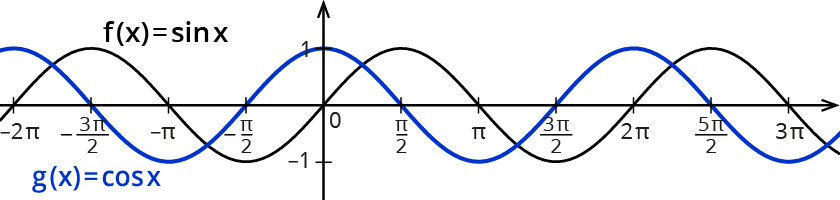
\includegraphics[width=\columnwidth]{Sinus_Kosinus_Eigenschaften}	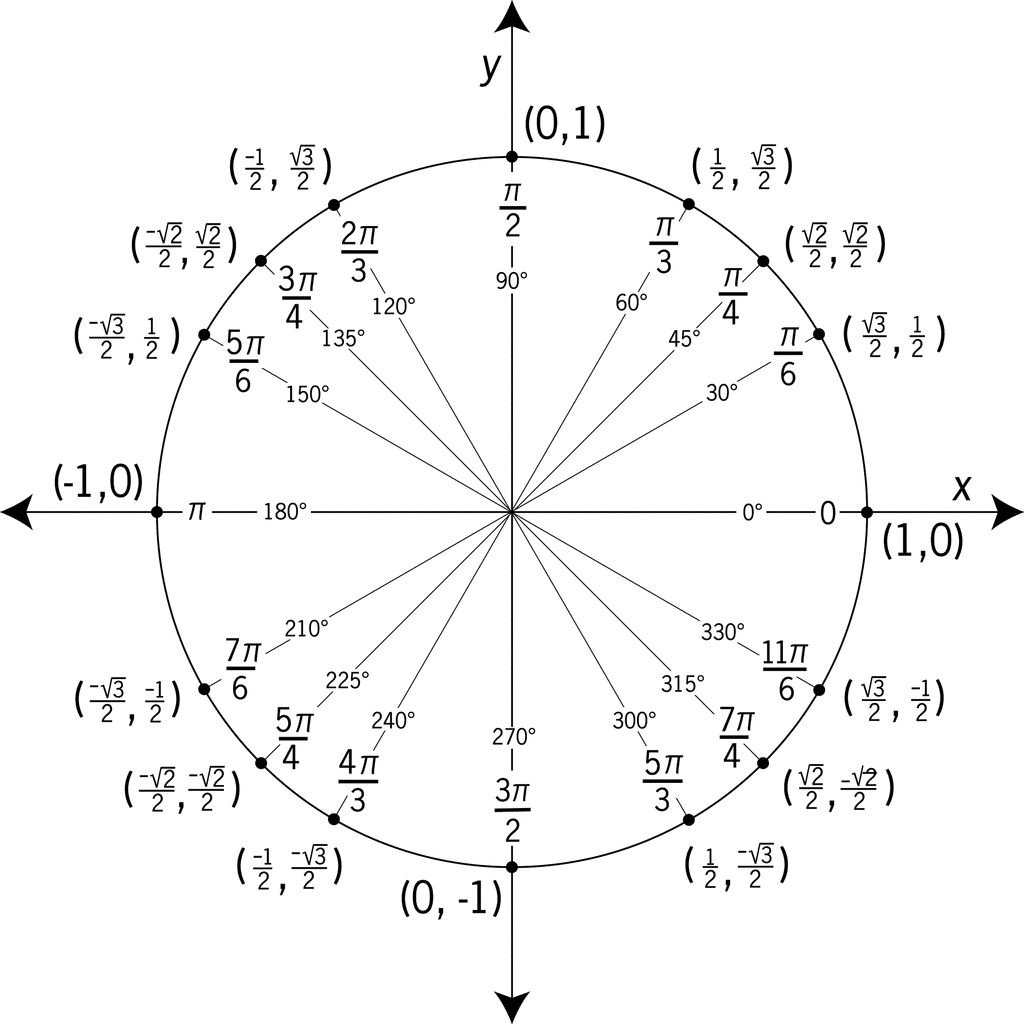
\includegraphics[width=0.65\columnwidth]{einheitskreis}
\clearpage
\newpage
\section{Signale im Zeitbereich}
  \subsection{Signalcharakterisierung}
  \begin{itemize}
      \item{\textbf{Kontinuierlich \hfill $\longleftrightarrow$ \hfill Diskret}}
      \item{\textbf{Deterministisch \hfill $\longleftrightarrow$ \hfill Stochastisch}}\\
          Deterministisch: $x(t)$ mathematisch beschreibbar.
          Stochastisch: Signal zufällig, kein $x(t)$.
      \item{\textbf{Periodisch \hfill $\longleftrightarrow$ \hfill Aperiodisch}}\\
              Periodisch, wenn $x(t)=x(k \cdot t+T_p)$ mit
			  $T_p = \frac{2\pi}{k}$ \\
              $T_p$: Grundperiode/Periodendauer
      \item{\textbf{Gerade $x(-t)=x(t)$ $\leftrightarrow$ Ungerade: $x(-t)=-x(t)$}}\\
          \begin{mdframed}[style=exercise,frametitle=Zerlegung des Signals:]
              - gerader Anteil: \quad $x_G=\frac{1}{2}\left[x(t)+x(-t)\right]$\\
              - ungerader Anteil: \quad $x_U=\frac{1}{2}\left[ x(t)-x(-t) \right]$\\
              - gemischtes Signal: $x(t)=x_G + x_U$
          \end{mdframed}
          \begin{center}
              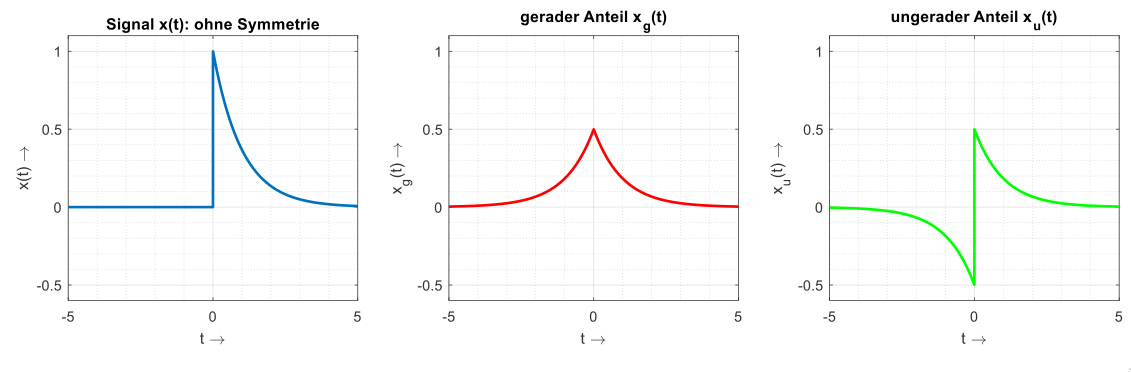
\includegraphics[width=0.43\textwidth]{Signale/gerade_ungerade_signal}
          \end{center}
      \item{\textbf{Energie \hfill $\longleftrightarrow$ \hfill Leistung}}\\
              (Gesamt-)Energie: \[E_x=\int_{t=-\infty}^{+\infty}\lvert x(t)\rvert^2 dt\ \quad (0<E_x<\infty)\]
              Mittlere Leistung: \[P_x=\lim_{T\to\infty}\frac{1}{2T}\int_{-T}^{+T}\lvert x(t)\rvert^2 dt \quad (0<P_x<\infty)\]
                {\small Ein Signal ist nie Energie- und Leistungssignal gleichzeitig!}
          
      \item{\textbf{Korrelationsfunktion}}\\
          {\small Ma{\ss} f\"ur die \"Ahnlichkeit
          zweier Energiesignale.}
              \[
                  r_{xy}(\tau) = \int_{-\infty}^{\infty}x(t)\cdot y(t+\tau) dt
              \]
      \item{\textbf{Signaloperationen}}\\
        {\small Manipulation/Transformation mit folgenden Parametern:}
            \[ \boxed{
				f(t) = A \cdot f(\pm b \cdot (t \mp t_0)) \leftrightarrow A \cdot f\left(\frac{t\mp t_0}{b}\right)
				}
			\]
		 \renewcommand{\labelitemii}{$\bullet$}
          \begin{itemize}
              \item{Zeitverschiebung $t-t_0$: nach \textbf{rechts}}!

              \item{Zeitskalierung:\\
              	Multiplikation mit $b>1$: Stauchung \\
              	Multiplikation mit $0<b<1$: Dehnung \\
              	Division durch $b>0$: Dehnung}

              \item{Zeitumkehr/-invertierung:\\ $-1 \cdot b$: Spiegelung an y-Achse}
              \item{Signalinvertierung:\\
              $-A\cdot f(t)$: Spiegelung an x-Achse}
              
          \end{itemize}
          \textbf{Wichtig}: Reihenfolge beachten!\\
          Erst Verschieben, dann Skalieren/Invertieren!
  \end{itemize}
  \subsection{Elementarsignale}
  \begin{mdframed}[style=exercise]
      \begin{itemize}[leftmargin=*]
          \item{Sprung-, Heavyside-Fkt., Einheitssprung $\varepsilon$, $\sigma$}
          \[ \varepsilon(t) = \varepsilon(k\cdot t) = 
             \begin{cases}
                 0 & \text{f\"ur } t < 0\\
                 1 & \text{f\"ur } t \geq 0
             \end{cases}
          \]
Verschoben, Start bei $t_0$:
        \[ \varepsilon(t-t_0) = 
          \begin{cases}
          	0 & \text{f\"ur } t_0 < 0\\
          	1 & \text{f\"ur } t_0 \geq 0
          \end{cases}
          \]
          \item{Dirac-Impuls $\delta$}
          \[
              \int_{t=-\infty}^{\infty} \delta(t) \, dt = 1
          \]
          \begin{itemize}
              \item Höhe = $\infty$, Fläche = 1.
              \item{Zusammenhang mit Sprungfunktion:}\\
                  $\boxed{\int_{\tau=-\infty}^{t}\delta(\tau)d\tau =
                  \varepsilon(t)}$
                  $\boxed{\dfrac{d}{dt}\varepsilon(t) =
                  \delta(t)}$
              \item{\textbf{Ausblend}eigenschaft}:
                  \[
                      \int_{-\infty}^{\infty}\delta(t-t_0)\cdot y(t) = y(t_0)
                  \]
              \item{Zeitskalierung: }
                  $\delta(at)=\dfrac{1}{\lvert a\rvert}\,\delta(t)$
          \end{itemize}
          \item{Dreieckimpuls $\Lambda$}
          Fläche = 1.
          \[ \Lambda(t) =
             \begin{cases}
                 0 & \text{f\"ur } \vert t\rvert > 1\\
                 1-|t| & \text{f\"ur } \vert t\rvert \leq 1
             \end{cases}
          \]
          \item{Rechteckfunktion $\operatorname{rect}$}\\
          $T:$ Breite
          \[ \hat{u} \cdot \operatorname{rect}\left(\frac{t}{T}\right) =
             \begin{cases}
                 \hat{u} & \text{f\"ur } \vert t\rvert \leq \frac{T}{2}\\
                 0 & \text{f\"ur } \vert t\rvert > \frac{T}{2}
             \end{cases}
          \]
          Darstellbar durch:\\ $1\cdot  \operatorname{rect}(t) = \varepsilon\cdot\left( t+\frac{1}{2} \right)-\varepsilon\cdot\left( t-\frac{1}{2} \right)$
          \item{Komplexe Exponentialfunktion}\\
          siehe Kap. \ref{ufkt}.
          \[ x(t)=\underline{A}\cdot e^{st} = \underline{A}\cdot e^{(\sigma+j\omega)t} = |\underline{A}|\cdot e^{j\varphi} \cdot e^{(\sigma+j\omega)t}
          \]
          \item Si-Funktion
                    \[ \operatorname{si}(x) =
          \begin{cases}
          	\dfrac{\sin(x)}{x} & \text{f\"ur } x\neq 0\\
          	1 & \text{f\"ur } x = 0
          \end{cases}
          \]
          Nullstellen: $\operatorname{si}(k\pi)=0$ für $k\ge1,\, k\in \mathbb{Z}$
      \end{itemize}
  \end{mdframed}

\section{Systeme}
\subsection{Eigenschaften}
\begin{enumerate}
  \item{\textbf{Speicher}}\\
      % \begin{mdframed}[style=exercise]
          \bulletpt Frei: wird durch eine xy-Kennlinie vollständig
          beschrieben
          \[
              \text{z.B. \ }y(t)=\frac{R_1}{R_1+R_2}\cdot x(t)
          \]
          \bulletpt behaftet: Bei diesen Systemen ist keine
          vollständige Beschreibung durch eine xy-Kennline möglich
          \[
              \text{z.B. \ }y(t) = x(t)+2x(t-1)
          \]
      % \end{mdframed}
  \item{\textbf{Kausalit\"at}}\\
      % \begin{mdframed}[style=exercise]
           Ausgangssignal hängt nur vom aktuellen und vorherigen
           Eingangssignal ab
          \[
              \text{Kausal: z.B. \ }y(t) =
              \int\displaylimits_{t-5}^{t}x(\tau)d\tau
          \]
          \[
              \text{Akausal: z.B. \ }y(t) = x(t+1)-x(t-1)
          \]
      % \end{mdframed}

      \underline{Speicherfreiheit \& Kausalit\"at:} Aus Speicherfreiheit
      folgt Kausalität, aber nicht umgekehrt.
  \item{\textbf{Stabilit\"at}}\\
  (Bounded Input $\rightarrow$ Bounded Output)\\BIBO Stabilit\"at:
  kleines/beschr\"anktes Eingangssignal $\rightarrow$ kleine/beschr\"ankte
  Antwort.\\
  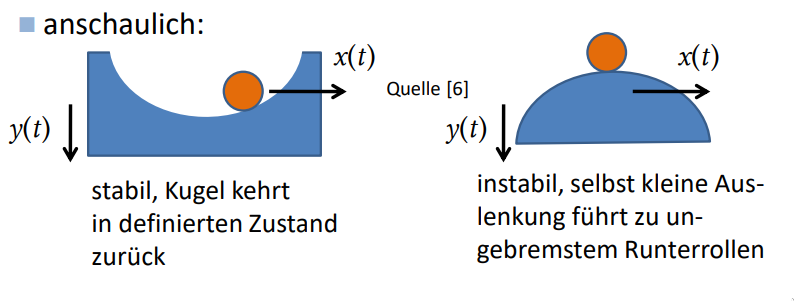
\includegraphics[width=.9\columnwidth]{Systeme/BIBO_anschaulich}\\
  % \begin{mdframed}[style=exercise]
      z.B. f\"ur stabiles System
  \[
      y(t) = 50\cdot x^3(t)
  \]\\
      z.B. f\"ur instabiles System
  \[
      y(t) = e^{t}\cdot x(t)
  \]
  % \end{mdframed}
  \item{\textbf{Zeitinvariant$\leftrightarrow$Zeitvariant}}\\
  \bulletpt invariant: Systeme \"andern sich \textbf{nicht} bei einer
  Zeitverschiebung.\\
  \bulletpt variant: Verschobenes Eingangssignal $\rightarrow$
  verschobenes Ausgangssignal
  \item{\textbf{Liniarit\"at}}\\
      Ein System ist linear, wenn das Superpositionsprinzip gilt:
      Linearkombination von Eingangssignalen ruft entsprechende
      Linearkombination der Ausgangssignale hervor
      \begin{mdframed}[style=exercise,frametitle=Bedeutung Liniarit\"at]
          eine Verdopplung der Eingangsgröße (z.B. Spannung) führt auch zu
          einer Verdopplung der Ausgangsgröße.
      \end{mdframed}
\end{enumerate}
\subsection{LTI-Systeme (Linear time-invariant Systems)}
\subsubsection{Ein-/Ausgangsbeziehung}
\begin{itemize}
  \item Addition
  \item Multiplikation
  \item Differentiation
  \item Integration
  \item Zeitverschiebung(Verz\"ogerung)
\end{itemize}
\subsubsection{Faltung}
Aus der Impulsantwort eines LTI-Systems und dem Eingangssignal lässt sich das
Ausgangssignal durch Faltung bestimmen:
\begin{mdframed}[style=exercise]
  \[
      y(t)=x(t)*h(t) \rightarrow (*)\text{ Faltung Operator}
  \]
  \[
      \boxed{y(t) = \int_{-\infty}^{+\infty} x(\tau)\cdot h(t-\tau)d\tau}
  \]
  \bulletpt Der Dirac-Impuls ist das neutrale Element der Faltung
  \[
      x(t)*\delta(t)=x(t)
  \]
  \bulletpt Eine Faltung mit einem verschobenen Dirac-Impuls führt zur Verschiebung
  des Signals:
  \[
      x(t)* \delta(t - a) = x(t - a)
  \]
\end{mdframed}
\begin{mdframed}[style=exercise,frametitle=Rechenregeln]
  \begin{itemize}
      \item{$x_1(t)*x_2(t)=x_2(t)*x_1(t)$}
      \item{$x_1(t)*[x_2(t)*x_3(t)]=[x_1(t)*x_2(t)]*x_3(t)$}
      \item{$x_1(t)*[x_2(t)+x_3(t)]=x_1(t)*x_2(t)+x_1(t)*x_3(t)$}
  \end{itemize}
\end{mdframed}
\subsection{Frequenzgang \& \"Ubertragungsfunktion}
\begin{mdframed}[style=exercise]
  \begin{itemize}
      \item{\textbf{Frequenzgang}}\\
          \[
              \underline{H}(\omega) =
              \frac{\underline{Y}(\omega)}{\underline{X}(\omega)} =
              \frac{\underline{U_2}(\omega)}{\underline{U_1}(\omega)}
          \]
      \item{\textbf{Amplitudengang}}\\
          \[
              A(\omega) = |\underline{H}(\omega)| =
              \frac{|\underline{Y}(\omega)|}{|\underline{X}(\omega)|}
              \begin{cases}
                  > 1 & \text{Verst\"arkung}\\
                  < 1 & \text{D\"ampfung}
              \end{cases}
          \]
      \item{\textbf{Phasengang}}\\
          \[
              \varphi_H(\omega) = \text{arg}\{\underline{H}(\omega)\} =
              \varphi_Y(\omega) - \varphi_X(\omega)
          \]
          \[
              \varphi_H = \text{arctan}(\frac{\mathfrak{Im}}{\mathfrak{Re}})
          \]
      \item{\textbf{Eigenfunktion}}\\
          \[
              y(t) = \lambda\cdot x(t)
              \begin{cases}
                  x(t): & \text{Eigenfunktion}\\
                  \lambda: & \text{Eigenwert}(\lambda\in\mathbb{C})
              \end{cases}
          \]
  \end{itemize}
\end{mdframed}
\begin{mdframed}[style=exercise]
  jede komplexe Exponentialfunktion $x(t) = \e^{st}$ ist Eigenfunktion
  jedes beliebigen LTI-Systems $S$:
  \[
      y(t) = S\left\{ \e^{st} \right\} = \lambda\cdot \e^{st}
  \]
  Eigenwert kann wie folgt berechnet werden:
  \[
      \lambda = \underline{H}(s) = \int_{-\infty}^{+\infty} h(\tau)\  \e^{-st} d\tau
  \]
  \begin{itemize}
      \item{\textbf{Erweiterung der komplexen Wechselstromrechnung}}\\
          Die harmonische Exponentialfunktion $e^{j\omega t}$ ist ein
          sonderfall von $e^{st}$ mit $s=j\omega$
          \[
              \sigma \triangleq Amplitude
              \begin{cases}
                  \sigma \leq 0 & \text{exponentiell abklingend}\\
                  \sigma = 0 & \text{konstante Amplitude}\\
                  \sigma \geq 0 & \text{exponentiell zunehmend}
              \end{cases}
          \]
          \[
              \omega \triangleq Rotation
              \begin{cases}
                  \omega \leq 0 & \text{Zeiger rotiert mit UZS}\\
                  \omega = 0 & \text{Zeiger rotiert nicht}\\
                  \omega \geq 0 & \text{Zeiger rotiert gegen UZS}
              \end{cases}
          \]
  \end{itemize}
\end{mdframed}
% \[
%   \boxed{
%   \begin{circuitikz}[scale=1,transform shape]
%       \draw(0,0) to[generic] node[anchor=east,yshift=-20pt]{$\underline{Z}(s)\mathrm{=}R$} (2,0);
%       \draw(3,0) to[L] node[anchor=east,yshift=-20pt, xshift=5pt]{$\underline{Z}(s)\mathrm{=}s\cdot L$} (5,0);
%       \draw(6,0) to[C, l=] node[anchor=east, yshift=-20pt, xshift=6pt]{$\underline{Z}(s)\mathrm{=}\frac{1}{s\cdot C}$} (8,0);
%   \end{circuitikz}
%   }
% \]

\begin{mdframed}[style=exercise,frametitle=Komplexe \"Ubertragungsfunktion]
  \footnotesize
  \[
      \underline{H}(s)=\frac{\underline{Y}(s)}{\underline{X}(s)}=\frac{\underline{U_2}(s)}{\underline{U_1}(s)}=\frac{\text{komplexer
      Zeiger des Ausgangssignals}}{\text{komplexer Zeiger des
      Eingangssignals}}
  \]
  \normalsize
  Die Übertragungsfunktion hängt von der komplexen\linebreak Frequenz
  $s=\sigma+j\omega$ ab.
\end{mdframed}

\subsubsection{Pegel}
    \begin{mdframed}[style=exercise]
        Energiegröße: $\quad a = 10\cdot \lg\dfrac{P_1}{P_2}dB $\\
        Feldgröße: $\qquad a = 20\cdot \lg\dfrac{U_1}{U_2}dB $
    \end{mdframed}

\subsection{Pole und Nullstellen}
\[
    H(s)=\frac{\sum_{m=0}^{M} b_{m} \cdot s^{m}}{\sum_{n=0}^{N} a_{n} \cdot s^{n}}
\]
Die Koeffizienten an und bm ergeben sich aus den Bauelementen und sind reell.
\begin{mdframed}[style=exercise]
    \begin{align*}
        \underline{H}(s) &= \frac{\textsc{Summe aller Nullstellen}}{\textsc{Summe aller Pole}}\\
        &=\frac{b_{M}}{a_{N}} \cdot \frac{\left(s-s_{o 1}\right) \cdot\left(s-s_{o
        2}\right) \cdot \ldots \cdot\left(s-s_{o M}\right)}{\left(s-s_{x 1}\right)
        \cdot\left(s-s_{x 2}\right) \cdot \ldots \cdot\left(s-s_{x N}\right)}
    \end{align*}
    $k=\dfrac{b_M}{a_N}$ ist der Maßstabfaktor
\end{mdframed}
\textbf{Bei stabilen Systemen müssen alle Pole in der linken komplexen Halbebene liegen.}

\subsection{Elementare Übertragungsglieder}
\footnotesize
    P-Glied , D-Glied , I-Glied , PT1-Glied
\normalsize
Für mehr sehe externe Tabelle.

\subsection{Zusammenschalten von Übertragungsgliedern}
\begin{mdframed}[style=exercise]
\begin{itemize}
    \item Kettenschaltung\\
        \textbf{Multiplikation} der Einzelübertragungsfunktionen.
        \[
            \boxed{\underline{H}_{e}(s)=\underline{H}_{B}(s) \cdot \underline{H}_{A}(s)=\underline{H}_{A}(s) \cdot \underline{H}_{B}(s)}
        \]
        \begin{center}
            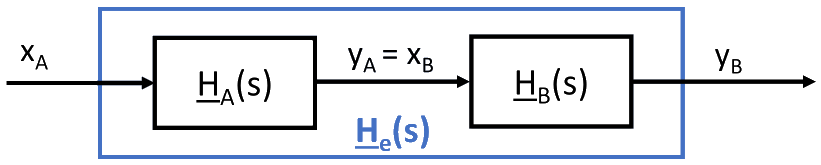
\includegraphics[width=0.7\columnwidth]{Kettenschaltung_Uebertragungsglieder}
            \[
                \underline{Y}_{B}=\underline{H}_{B}(s) \cdot \underline{X}_{B}=\underline{H}_{B}(s) \cdot \underline{Y}_{A}=\underline{H}_{B}(s) \cdot \underline{H}_{A}(s) \cdot \underline{X}_{A}
            \]
        \end{center}
        Rückwirkungsfreiheit gewährleistet sein.
    \item Parallelschaltung\\
        \textbf{Summe} der Einzelübertragungsfunktionen.
        \[
            \boxed{\underline{H}_{e}(s)=\underline{H}_{B}(s) + \underline{H}_{A}(s)}
        \]
        \begin{center}
            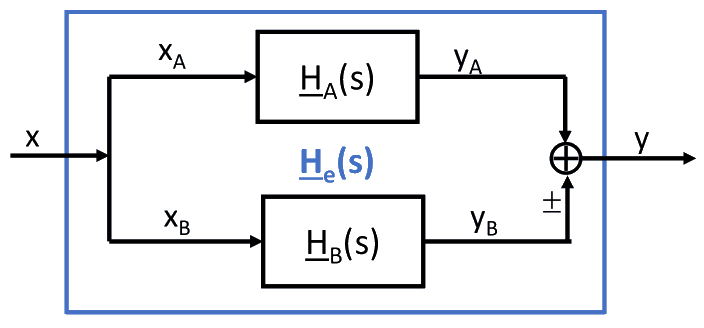
\includegraphics[width=0.6\columnwidth]{Parallel_Uebertragungsglieder}
            \begin{align*}
                \underline{Y}&=\underline{Y}_{A} \pm \underline{Y}_{B}\\
                             &=\underline{H}_{A}(s) \cdot \underline{X}_{A} \pm \underline{H}_{B}(s) \cdot \underline{X}_{B}\\
                             &=\left(\underline{H}_{A}(s)+\underline{H}_{B}(s)\right) \cdot \underline{X}
            \end{align*}
        \end{center}
    \item Rückkopplung
        \[
            \boxed{\underline{H}_{e}(s)=\frac{\underline{H}_{A}(s)}{1\pm\underline{H}_{A}(s) \cdot \underline{H}_{B}(s)}}
        \]
        \begin{center}
            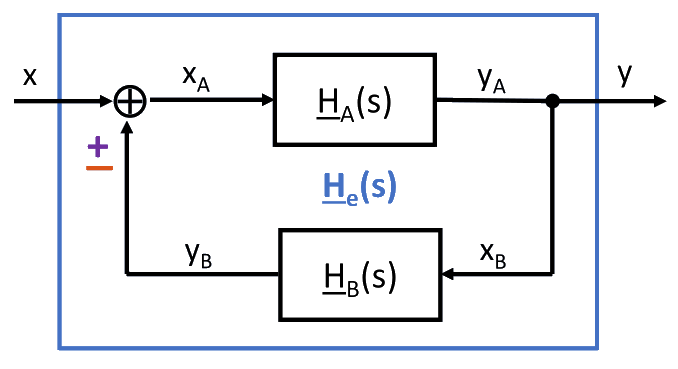
\includegraphics[width=0.6\columnwidth]{Rueckkopplung_Uebertragungsglieder}\\
            Mitkopplung: $y_A$ vergrößert $x_A$\\
            Gegenkopplung $y_A$ verkleinert $x_A$
        \end{center}

\end{itemize}
\end{mdframed}

\subsection{Bode Diagramm}
\begin{itemize}
    \item Bode Diagramm von Kettenschaltung\\
        Ergibt sich durch \textbf{Addition der Bodediagramme} der einzelnen Glieder.
    \item Bode Diagramm der inversen Übertragungsfunktion\\
        Ergibt sich durch \textbf{Spiegelung an der X-Achse}.
\end{itemize}

\clearpage
\section{Zweitore, Vierpole}
\subsection{Zweitorgleichungen}
%\small
% \includegraphics[width=\columnwidth]{Zweipole/Zweitorgleichungen}
    \begin{itemize}[leftmargin=*]
        \item{Admittanzform/ Admittanzmatrix \textbf{Y}:}
        \begin{align*}
            \begin{split}
                \underline{I}_1 &= \underline{Y}_{11}\cdot\underline{U}_1 + \underline{Y}_{12}\cdot\underline{U}_2\\
                \underline{I}_2 &= \underline{Y}_{21}\cdot\underline{U}_1 + \underline{Y}_{22}\cdot\underline{U}_2
            \end{split} \qquad
            {\small\begin{pmatrix}
                \underline{I}_1 \\
                \underline{I}_2
            \end{pmatrix}} = \textbf{\underline{Y}}\cdot
            \begin{pmatrix}
                \underline{U}_1 \\
                \underline{U}_2
            \end{pmatrix}      
        \end{align*}
        \item{Impedanzform/ Impedanzmatrix \textbf{Z}:}
            \begin{align*}
                \begin{split}
                \underline{U}_1 &=\underline{Z}_{11}\cdot\underline{I}_1 + \underline{Z}_{12}\cdot\underline{I}_2 \\
                \underline{U_2} &=\underline{Z}_{21}\cdot\underline{I}_1 + \underline{Z}_{22}\cdot\underline{I}_2
                \end{split}\qquad
                \begin{pmatrix}
                    \underline{U}_1 \\
                    \underline{U}_2
                \end{pmatrix} = \textbf{\underline{Z}}\cdot
                \begin{pmatrix}
                    \underline{I}_1 \\
                    \underline{I}_2
                \end{pmatrix}  
            \end{align*}
        \item{Hybridform 1/ Reihenparallelmatrix \textbf{H}:}
            \begin{align*}
                \begin{split}
                    \underline{U}_1 &= \underline{H}_{11}\cdot\underline{I}_1 + \underline{H}_{12}\cdot\underline{U}_2 \\
                    \underline{I}_2 &= \underline{H}_{21}\cdot\underline{I}_1 + \underline{H}_{22}\cdot\underline{U}_2
                \end{split}
				\qquad	
                \begin{pmatrix}
                    \underline{U}_1 \\
                    \underline{I}_2
                \end{pmatrix} = \textbf{\underline{H}}\cdot
                \begin{pmatrix}
                    \underline{I}_1 \\
                    \underline{U}_2
                \end{pmatrix}
            \end{align*}
            \item{Hybridform 2/ Parallelreihenmatrix \textbf{C}:}
            \begin{align*}
                \begin{split}
                    \underline{I}_1 &= \underline{C}_{11}\cdot\underline{U}_1 + \underline{C}_{12}\cdot\underline{I}_2 \\
                    \underline{U}_2 &= \underline{C}_{21}\cdot\underline{U}_1 + \underline{C}_{22}\cdot\underline{I}_2
                \end{split}
				\qquad
                \begin{pmatrix}
                    \underline{I}_1 \\
                    \underline{U}_2
                \end{pmatrix} = \textbf{\underline{C}}\cdot
                \begin{pmatrix}
                    \underline{U}_1 \\
                    \underline{I}_2
                \end{pmatrix}
            \end{align*}
            
            \item{Kettenform/ Kettenmatrix \textbf{A}:}
                \begin{align*}
                    \begin{split}
                        \underline{U}_1 &= \underline{A}_{11}\cdot\underline{U}_2 + \underline{A}_{12}\cdot-\underline{I}_2 \\
                        \underline{I}_1 &= \underline{A}_{21}\cdot\underline{U}_2 + \underline{A}_{22}\cdot-\underline{I}_2
                    \end{split}
	               \qquad
                    \begin{pmatrix}
                        \underline{U}_1 \\
                        \underline{I}_2
                    \end{pmatrix} = \textbf{\underline{A}}\cdot
                    \begin{pmatrix}
                        \underline{U}_2 \\
                        -\underline{I}_2
                    \end{pmatrix}
                \end{align*}
                \item{Kettenform rückwärts/ Kettenmatrix \textbf{B}:}
                    \begin{align*}
                        \begin{split}
                            \underline{U}_2 &= \underline{B}_{11}\cdot\underline{U}_1 + \underline{B}_{12}\cdot-\underline{I}_1\\
                            \underline{I}_2 &= \underline{B}_{21}\cdot\underline{U}_1 + \underline{B}_{22}\cdot-\underline{I}_1
                        \end{split}
                    \qquad
                    \begin{pmatrix}
                        \underline{U}_2\\
                        \underline{I}_2
                    \end{pmatrix} = \textbf{\underline{B}}\cdot
                    \begin{pmatrix}
                        \underline{U}_1 \\
                        -\underline{I}_1
                    \end{pmatrix}
                    \end{align*}
    \end{itemize}
   \normalsize
\subsubsection{Parameterumrechnung}
\begingroup
\arraycolsep=1.0pt\def\arraystretch{2.0}
\begin{align*}
    Z && \hspace{0.5cm} Y && \hspace{0.5cm} H && \hspace{0.5cm} A
\end{align*}
\[
    Z\
    \begin{bmatrix}
        \underline{Z}_{11} & \underline{Z}_{12}\\
        \underline{Z}_{21} & \underline{Z}_{22}
    \end{bmatrix}
    \begin{bmatrix}
        \dfrac{\underline{Y}_{22}}{\operatorname{det}\underline{\boldsymbol{Y}}} & \dfrac{-\underline{Y}_{12}}{\operatorname{det} \underline{\boldsymbol{Y}}}\\
        \dfrac{-\underline{Y}_{21}}{\operatorname{det} \underline{\boldsymbol{Y}}} & \dfrac{\underline{{Y}}_{11}}{\operatorname{det} \underline{\boldsymbol{Y}}} \\
    \end{bmatrix}
    \begin{bmatrix}
        \dfrac{\operatorname{det}\underline{\boldsymbol{{H}}}}{\underline{H}_{22}} & \dfrac{\underline{H}_{12}}{\underline{H}_{22}} \\
        \dfrac{-\underline{H}_{21}}{\underline{H}_{22}} & \dfrac{1}{\underline{H}_{22}}
    \end{bmatrix}
    \begin{bmatrix}
        \dfrac{\underline{A}_{11}}{\underline{A}_{21}} & \dfrac{\operatorname{det}\underline{\boldsymbol{A}}}{\underline{A}_{21}}\\
        \dfrac{1}{\underline{A}_{21}} & \dfrac{\underline{{A}}_{22}}{\underline{A}_{21}} \\
    \end{bmatrix}
\]
\[
    Y\
    \begin{bmatrix}
        \dfrac{\underline{Z}_{22}}{\operatorname{det}\underline{\boldsymbol{Z}}} & \dfrac{-\underline{Z}_{12}}{\operatorname{det} \underline{\boldsymbol{Z}}}\\
        \dfrac{-\underline{Z}_{21}}{\operatorname{det} \underline{\boldsymbol{Z}}} & \dfrac{\underline{{Z}}_{11}}{\operatorname{det} \underline{\boldsymbol{Z}}} \\
    \end{bmatrix}
    \begin{bmatrix}
        \underline{Y}_{11} & \underline{Y}_{12}\\
        \underline{Y}_{21} & \underline{Y}_{22}
    \end{bmatrix}
    \begin{bmatrix}
        \dfrac{1}{\underline{H}_{11}} & \dfrac{-\underline{H}_{12}}{\underline{H}_{11}} \\
        \dfrac{\underline{H}_{21}}{\underline{H}_{11}} & \dfrac{\operatorname{det}\underline{\boldsymbol{{H}}}}{\underline{H}_{11}}
    \end{bmatrix}
    \begin{bmatrix}
        \dfrac{\underline{A}_{22}}{\underline{A}_{12}} & \dfrac{-\operatorname{det}\underline{\boldsymbol{A}}}{\underline{A}_{12}}\\
        \dfrac{-1}{\underline{A}_{12}} & \dfrac{\underline{{A}}_{11}}{\underline{A}_{12}} \\
    \end{bmatrix}
\]
\[
    H\
    \begin{bmatrix}
        \dfrac{\operatorname{det}\underline{\boldsymbol{{Z}}}}{\underline{Z}_{22}} & \dfrac{\underline{Z}_{12}}{\underline{Z}_{22}} \\
        \dfrac{-\underline{Z}_{21}}{\underline{Z}_{22}} & \dfrac{1}{\underline{Z}_{22}}
    \end{bmatrix}
    \begin{bmatrix}
        \dfrac{1}{\underline{Y}_{11}} & \dfrac{-\underline{Y}_{12}}{\underline{Y}_{11}} \\
        \dfrac{\underline{Y}_{21}}{\underline{Y}_{11}} & \dfrac{\operatorname{det}\underline{\boldsymbol{{Y}}}}{\underline{Y}_{11}}
    \end{bmatrix}
    \begin{bmatrix}
        \underline{H}_{11} & \underline{H}_{12}\\
        \underline{H}_{21} & \underline{H}_{22}
    \end{bmatrix}
    \begin{bmatrix}
        \dfrac{\underline{A}_{12}}{\underline{A}_{22}} & \dfrac{\operatorname{det}\underline{\boldsymbol{A}}}{\underline{A}_{22}}\\
        \dfrac{-1}{\underline{A}_{22}} & \dfrac{\underline{{A}}_{21}}{\underline{A}_{22}} \\
    \end{bmatrix}
\]
\[
    A\
    \begin{bmatrix}
        \dfrac{\underline{Z}_{11}}{\underline{Z}_{21}} & \dfrac{\operatorname{det}\underline{\boldsymbol{Z}}}{\underline{Z}_{21}}\\
        \dfrac{1}{\underline{Z}_{21}} & \dfrac{\underline{{Z}}_{22}}{\underline{Z}_{21}} \\
    \end{bmatrix}
    \begin{bmatrix}
        \dfrac{-\underline{Y}_{22}}{\underline{Y}_{21}} & \dfrac{-1}{\underline{Y}_{21}}\\
        \dfrac{-\operatorname{det}\underline{\boldsymbol{Y}}}{\underline{Y}_{21}} & \dfrac{-\underline{{Y}}_{11}}{\underline{Y}_{21}} \\
    \end{bmatrix}
    \begin{bmatrix}
        \dfrac{-\operatorname{det}\underline{\boldsymbol{{H}}}}{\underline{H}_{21}} & \dfrac{-\underline{H}_{11}}{\underline{H}_{21}} \\
        \dfrac{-\underline{H}_{22}}{\underline{H}_{21}} & \dfrac{-1}{\underline{H}_{21}}
    \end{bmatrix}
    \begin{bmatrix}
        \underline{A}_{11} & \underline{A}_{12}\\
        \underline{A}_{21} & \underline{A}_{22}
    \end{bmatrix}
\]
\endgroup


\subsection{Betriebsarten}

\subsection{Bezugspfeilsystem}

\subsection{ZT-Eigenschaften}
\small
\begin{tabularx}{0.85\columnwidth}{|c|c|c|X|}
	\hline
	& Umkehrbarkeit & Symmetrie & Rückwirkungs-freiheit\\
	\hline\hline
	$Z$&  $Z_{12} = Z_{21}$ & $Z_{11} = Z_{22}$ & $Z_{12} = 0$\\
	\hline
	$Y$&  $Y_{12} = Y_{21}$& $Y_{11} = Y_{22}$ & $Y_{12 } = 0$ \\
	\hline
	$A$&  $\operatorname{det}[A] = 1$& $A_{11} = A_{22}$ & $\operatorname{det}[A] = 0$\\
	\hline
	$H$&  $H_{12} = -H_{21}$& $\operatorname{det}[H]=1$ & $H_{12} = 0$ \\
	\hline
\end{tabularx}\\
\begin{itemize}[leftmargin=*]
	\item Umkehrbares (reziprokes) ZT: nur 3 Parameter.
	\item (Widerstands-)symmetrisches ZT: Eingangswiderstände in beiden Betriebsarten gleich, Ein- und Ausgang vertauschbar.
	\item Umkehrbares und symmetrisches ZT = längssymmetrisch: nur 2 Parameter.
	\item Passives ZT aus R,L,C,M-Bauteilen ist immer umkehrbar.
	\item Rückwirkungsfreies (unilaterales) ZT: nur 3 Parameter, Energieübertragung nur von Eingang auf Ausgang.
\end{itemize}
\clearpage
\begin{samepage}
    \subsection{Matrizen elementarer Zweitore}
    \begin{center}
    	\includegraphics[width=\textwidth]{Zweipole/Tabellen und Ergänzungen_Zweitormatrizen}
    \end{center}
\end{samepage}
\clearpage

\subsection{Zusammenschalten von Zweitoren}
\subsubsection{Torbedingungen}
\small
Erfüllung durch: ideale \"Ubertrager, Kurzschlussschleife, Parallelschaltung längs-symmetrischer Zweitore.
\normalsize
\subsubsection{Zweitor-Schaltungen}
Torbedingung muss für ZT-Schaltungen erfüllt sein!\\

\begin{minipage}{0.45\columnwidth}
		\centering Reihenschaltung
	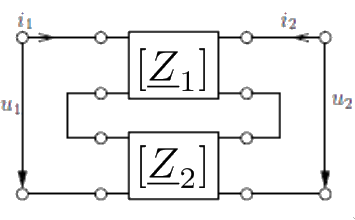
\includegraphics[width=0.8\columnwidth]{Zweipole/Reihenschaltung_Zweitore}
	\[
	\left[ \underline{Z} \right] = \left[ \underline{Z}_1 \right] + \left[ \underline{Z}_2 \right]
	\]
\end{minipage}
\begin{minipage}{0.45\columnwidth}
	\centering Parallelschaltung
	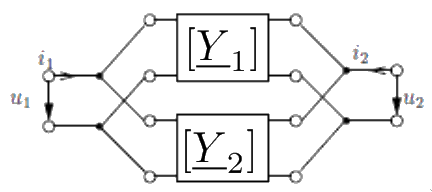
\includegraphics[width=\columnwidth]{Zweipole/Parallelschaltung_Zweitoren}
	\[
	\left[ \underline{Y} \right] = \left[ \underline{Y}_1 \right] + \left[ \underline{Y}_2 \right]
	\]
\end{minipage}  \\

\begin{minipage}{0.45\columnwidth}
			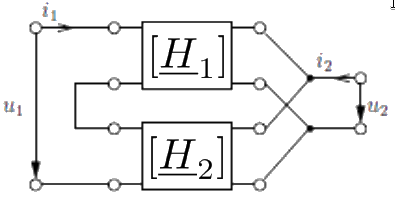
\includegraphics[width=\columnwidth]{Zweipole/Reihen-Parallelschaltung_Zweitoren}
			 Reihen-Parallelschaltung
	\[
	\left[ \underline{H} \right] = \left[ \underline{H}_1 \right] \cdot \left[ \underline{H}_2 \right]
	\]
\end{minipage}
\begin{minipage}{0.45\columnwidth}
			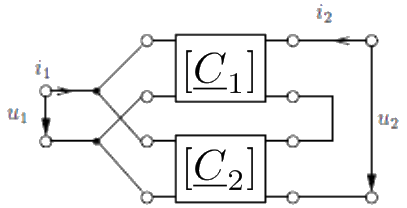
\includegraphics[width=\columnwidth]{Zweipole/Parallel-Reihenschaltung_Zweitoren}
			Parallel-Reihenschaltung
	\[
	\left[ \underline{C} \right] = \left[ \underline{C}_1 \right] \cdot \left[ \underline{C}_2 \right]
	\]
\end{minipage}

\begin{itemize}
	\item \textbf{Kettenschaltung}:\\
	Torbedingung wird immer eingehalten!
	\begin{center}
		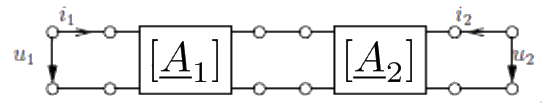
\includegraphics[width=0.6\columnwidth]{Zweipole/Kettenschaltung_Zweitoren}
		\[
		\left[ \underline{A} \right] = \left[ \underline{A}_1 \right] \cdot \left[ \underline{A}_2 \right] \neq \left[ \underline{A}_2
		\right] \cdot \left[ \underline{A}_1 \right]
		\]
	\end{center}
	\normalsize Reihenfolge beachten! \textbf{Nicht} kommutativ!
\end{itemize}
\subsubsection{Idealer Trennverst\"arker/OP} \label{trennverstärker}
Idealer Trennverstärker  $\text{v}_U$ als idealer OP.\\ 
Zweck: Rückwirkungsfreiheit der Kettenschaltung.\\
Entspricht einer VCVS.\\
\begin{minipage}{0.5\columnwidth}
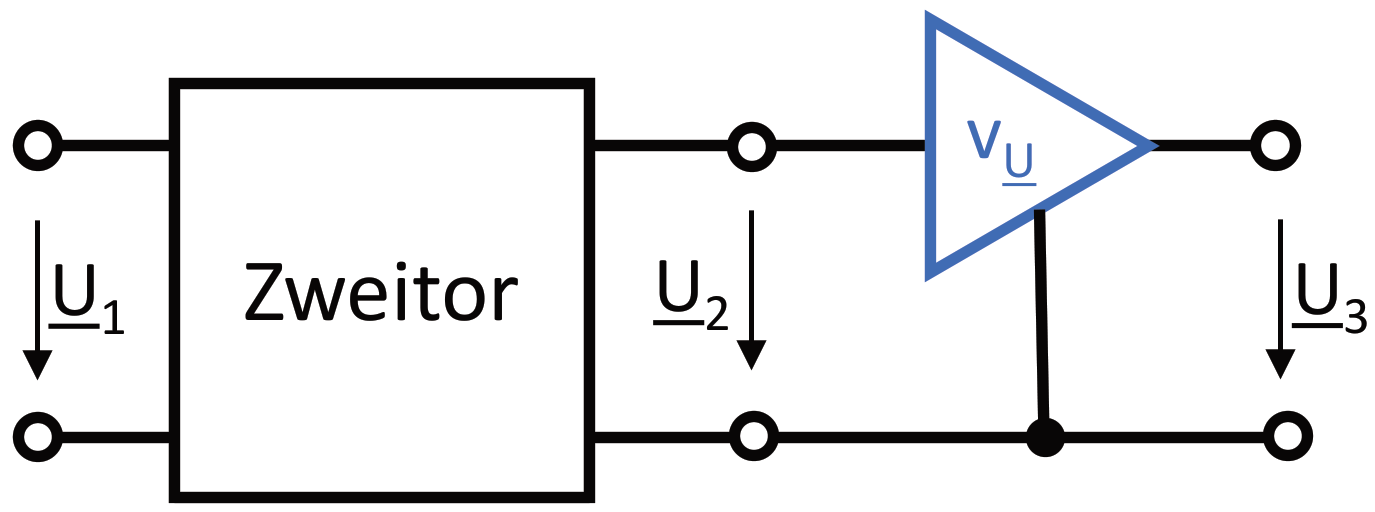
\includegraphics[width=1.2\columnwidth]{Zweipole/Trennverstaerker}
\end{minipage}
\begin{minipage}{0.5\columnwidth}
	\[
	[A] = \begin{pmatrix}
		\dfrac{1}{\text{v}_U} & 0 \\
		0        & 0
	\end{pmatrix}
	\]
\end{minipage}
\begin{equation*}
	\boxed{
	\underline{Z}_E \rightarrow \infty \quad \underline{Z}_A = 0 \quad \underline{\text{v}}_{\text{D}}=\underline{\text{v}}_U \rightarrow \infty }
\end{equation*}
\subsubsection{OP-Verstärker}
\begin{itemize}[leftmargin=*]
	\item nicht-inventierender OP\\
			\begin{minipage}{0.4\columnwidth}
				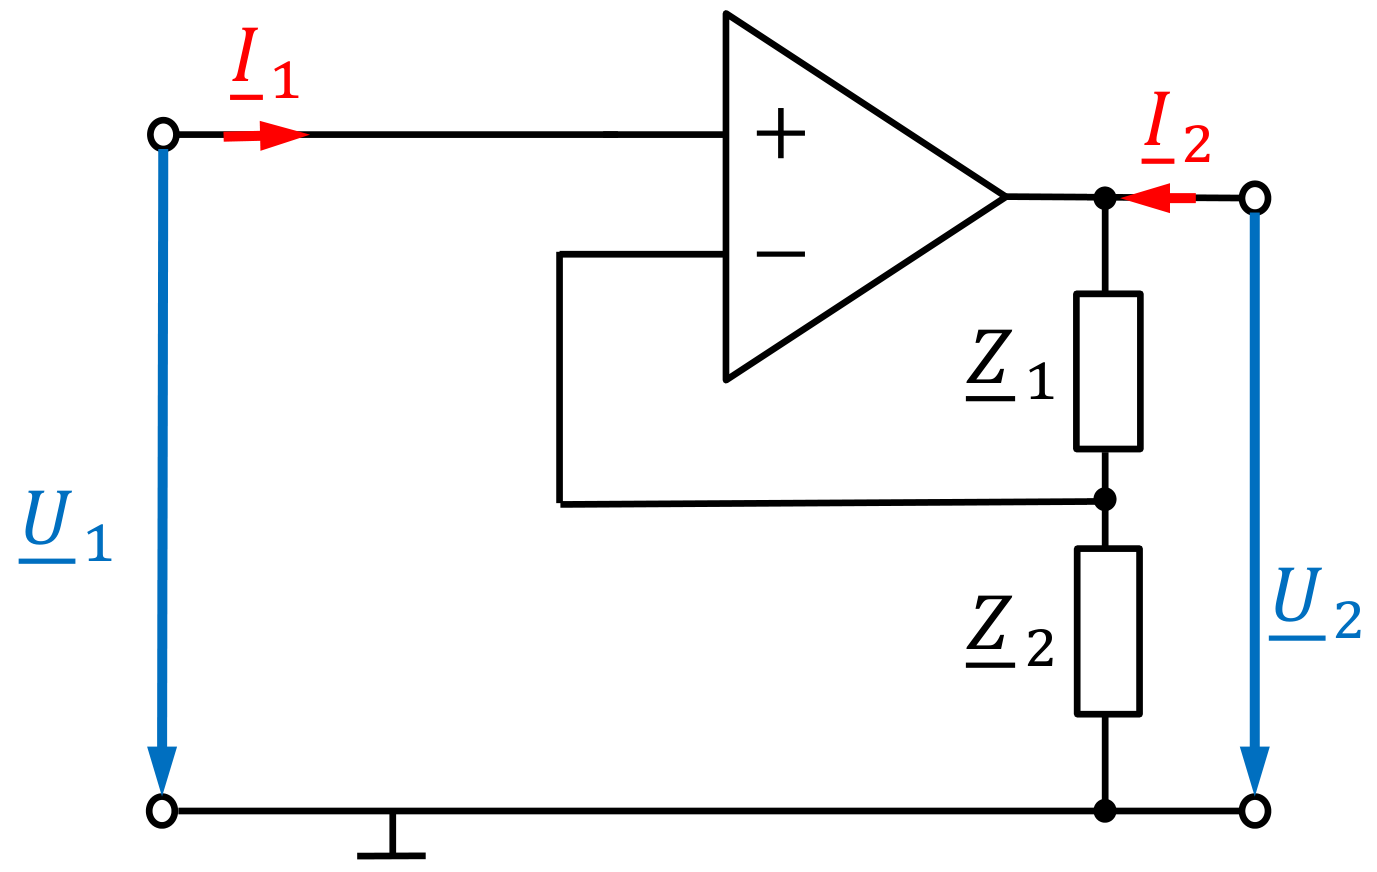
\includegraphics[width=\columnwidth]{Zweipole/nichtinventierender_op}
			\end{minipage}
			\begin{minipage}{0.6\columnwidth}
				\begin{equation*}
					A = \begin{pmatrix}
						\frac{1}{\nu_D} + \frac{Z_2}{Z_1 + Z_2} & \frac{Z_A}{\nu_D} \\
						\frac{1}{\nu_D Z_E} & \frac{Z_A}{\nu_D Z_E}
					\end{pmatrix}
				\end{equation*}
			Für idealen OP $\rightarrow$ \\
			$Z_E\rightarrow\infty, Z_A=0, v_D\rightarrow\infty$.
			\vspace{1.1em}
			\end{minipage}
			ideale Spannungs-Verstärkung:
			\begin{equation*}
				\text{v}_u=\frac{\underline{U}_2}{\underline{U}_1}=
				\frac{1}{\underline{A}_{11}}=\frac{\underline{Z}_1+\underline{Z}_2}{\underline{Z}_2} = 1 + \frac{Z_1}{Z_2}
			\end{equation*}
	\item inventierender OP\\
	\begin{minipage}{0.4\columnwidth}
		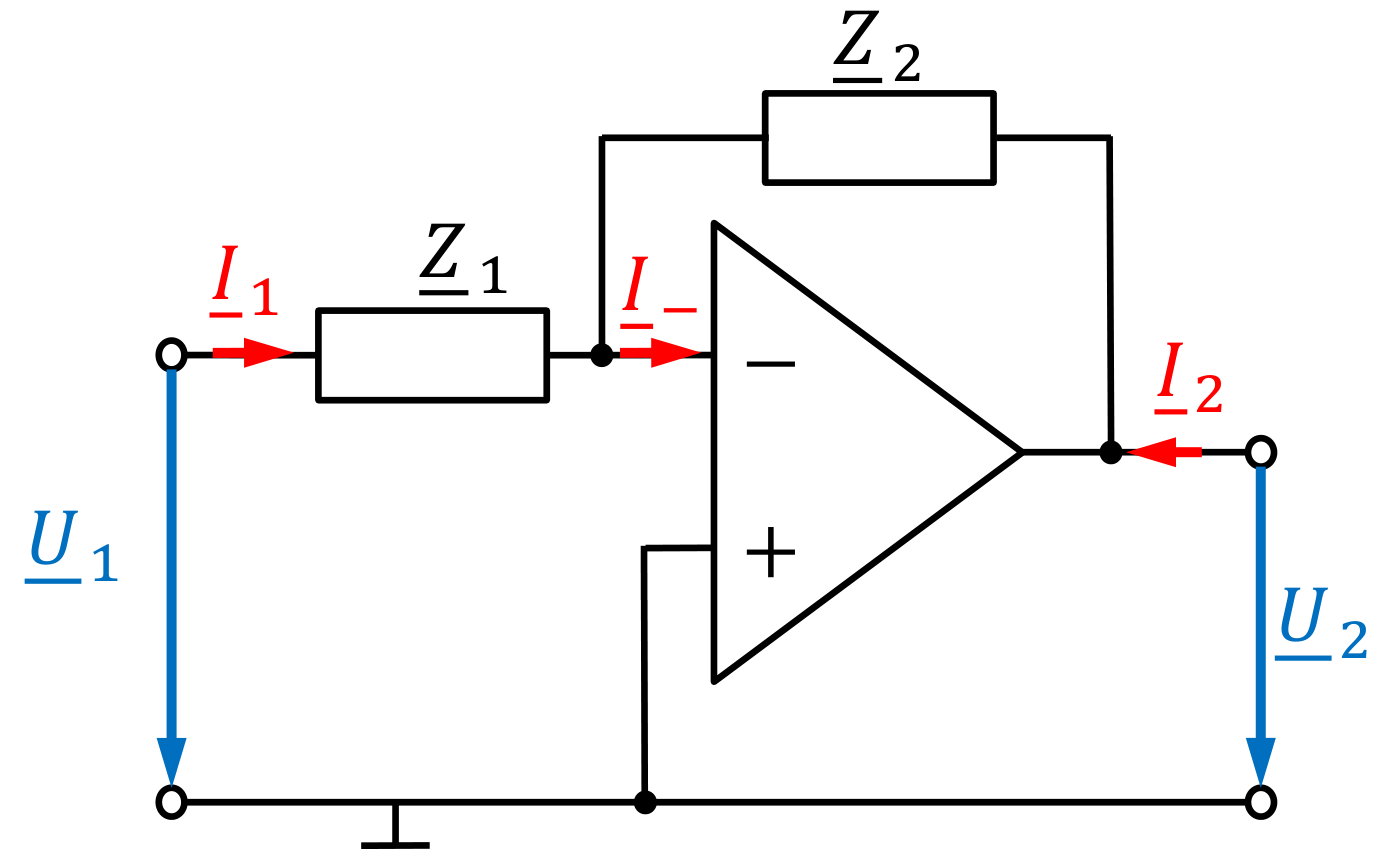
\includegraphics[width=\columnwidth]{Zweipole/inventierender_op}
	\end{minipage}
	\begin{minipage}{0.6\columnwidth}
		Allgemein, für idealen OP $\rightarrow$ \\
		$Z_E\rightarrow\infty, Z_A=0, v_D\rightarrow\infty$.
		\begin{equation*}
			A = \begin{pmatrix}
				\frac{1}{\nu_D} + \frac{Z_2}{Z_1 + Z_2} & \frac{Z_A}{\nu_D} \\
				\frac{1}{\nu_D Z_E} & \frac{Z_A}{\nu_D Z_E}
			\end{pmatrix}
		\end{equation*}
			\vspace{1em}
	\end{minipage}
			ideale Spannungs-Verstärkung:
	\begin{equation*}
		\text{v}_u=\frac{1}{\underline{A}_{11}}=\frac{\underline{U}_2}{\underline{U}_1}=-\frac{\underline{Z}_2}{\underline{Z}_1}
	\end{equation*}
\end{itemize}

\subsection{Ersatzschaltbilder}
\subsubsection{Ideale gesteuerte Quellen}
Ideale gesteuerte Quellen \textbf{nicht} ineinander umwandelbar! Andere Matrizen sind nicht definiert.\\
\begin{minipage}[t]{0.5\columnwidth}
\footnotesize
VCVS: Spannungsgesteuerte\\ Spannungsquelle
\normalsize
\begin{center}
	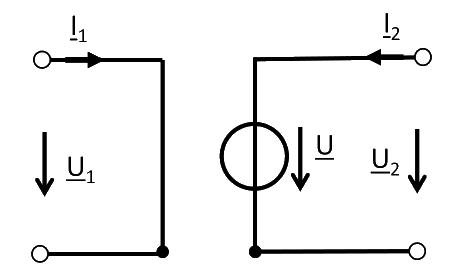
\includegraphics[width=0.9\columnwidth]{Zweipole/spg-spg-gestuert}\\
	\begin{tabular}{cc}
		VCVS:& $\underline{U}=\alpha\cdot \underline{U}_1$
	\end{tabular}
\end{center}
\end{minipage}
\begin{minipage}[t]{0.5\columnwidth}
 \footnotesize
	CCVS: Stromgesteuerte \\ Spannungsquelle
	\normalsize
	\begin{center}
		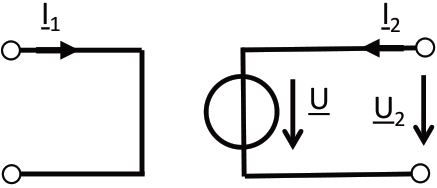
\includegraphics[width=0.9\columnwidth]{Zweipole/strm-spg-gestuert}\\
		\begin{tabular}{cc}
				CCVS: & $\underline{U}=\underline{Z}_T\cdot \underline{I}_1$
		\end{tabular}
	\end{center}
\end{minipage}
\begin{minipage}[t]{0.5\columnwidth}
	\footnotesize
	VCCS: Spannungsgesteuerte\\ Stromquelle
	\normalsize
	\begin{center}
		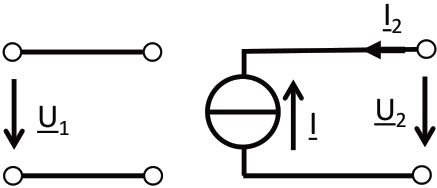
\includegraphics[width=0.9\columnwidth]{Zweipole/spg-strm-gestuert}\\
		\begin{tabular}{cc}
			VCCS:& $\underline{I}=\underline{Y}_T\cdot \underline{U}_1$
		\end{tabular}
	\end{center}
\end{minipage}
\begin{minipage}[t]{0.5\columnwidth}
	\footnotesize
	CCCS: Stromgesteuerte\\ Stromquelle
	\normalsize
	\begin{center}
		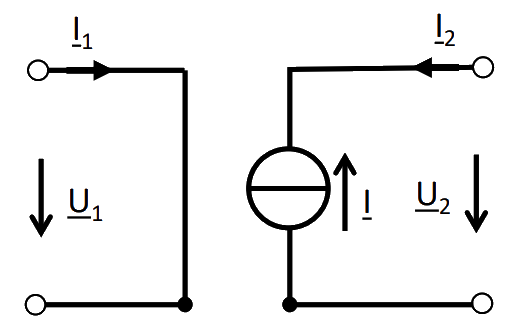
\includegraphics[width=0.9\columnwidth]{Zweipole/strm-strm-gesteuert}\\
		\begin{tabular}{cc}
			CCCS:& $\underline{I}=\beta\cdot \underline{I}_1$
		\end{tabular}
	\end{center}
\end{minipage}

\subsubsection{Lineare gesteuerte Quellen}
Alle Darstellungen sind äquivalent und lassen sich ineinander umwandeln! Andere Matrizen sind nicht definiert.\\
    \begin{minipage}{0.5\columnwidth}
    	\renewcommand{\arraystretch}{1.3}
        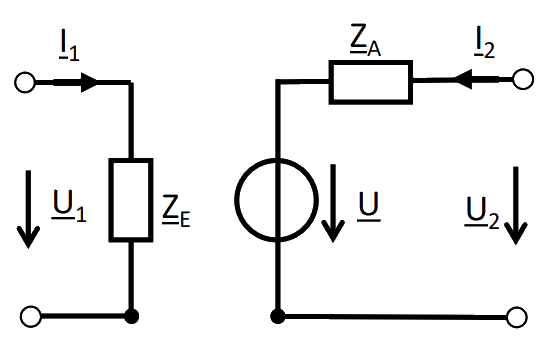
\includegraphics[width=0.9\columnwidth]{Zweipole/spg-spg-gestuert_linear}\\
    \begin{tabular}{ll}
        VCVS:& $\underline{U}=\alpha\cdot \underline{U}_1$\\
        CCVS:& $\underline{U}=\underline{Z}_T\cdot \underline{I}_1 $
    \end{tabular}
    \end{minipage}
    \begin{minipage}{0.5\columnwidth}
    	\renewcommand{\arraystretch}{1.3}
        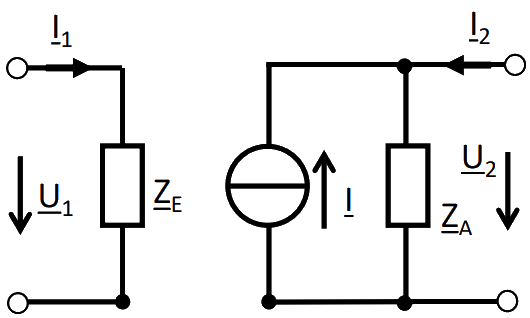
\includegraphics[width=0.9\columnwidth]{Zweipole/strm-strm-gesteuert_linear}\\
    \begin{tabular}{ll}
        CCCS:& $\underline{I}=\beta\cdot \underline{I}_1$\\
        VCCS:& $\underline{I}=\underline{Y}_T\cdot \underline{U}_1$
    \end{tabular}
    \end{minipage}
    
 \subsubsection{Matrizen für gesteuerte Quellen}   

\subsubsection{Ersatzschaltbilder (ESB)}
\begin{itemize}
    \item \textbf{T-ESB} bei gegebener $[\underline{Z}]$-Matrix:
   
    	$Z_{12} \neq Z_{21}$ mit gesteuerter Quelle. 
        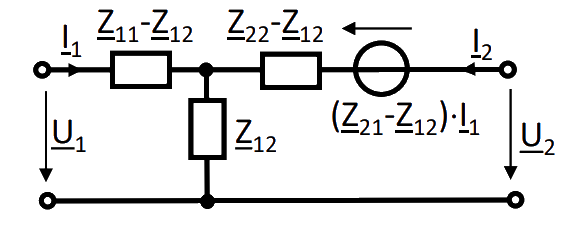
\includegraphics[width=0.7\columnwidth]{Zweipole/esb_t-mit_cs}
        \raggedright
        
    \item \textbf{$\Pi$-ESB} bei gegebener $[\underline{Y}]$-Matrix:
    
        $Y_{12} \neq Y_{21}$ mit gesteuerter Quelle.
        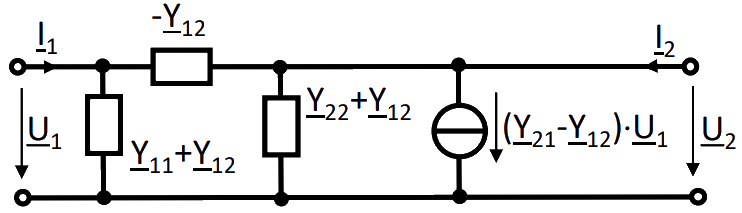
\includegraphics[width=0.8\columnwidth]{Zweipole/esb_pi-mit_cs}
        \raggedright
        
    \item  \textbf{Hybrid-ESB} bei gegebener [\underline{$H$}]-Matrix\\
    {\footnotesize Bsp.: ESB für NPN-Transistor.}
        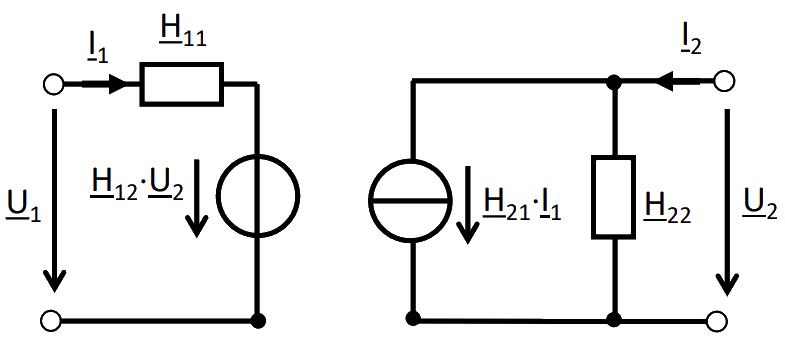
\includegraphics[width=0.7\columnwidth]{Zweipole/esb_hybrid-mit_cs}
\end{itemize}

\subsection{Beschaltete Zweitore}
\subsubsection{Ein- und Ausgangsimpedanz an Seite 1/2}
{\footnotesize $Z_V$: Last an Tor 2/ZT-Ausgang $\rightarrow$ Eingangsimpedanz, Betrieb von Seite 1\\ $Z_i$: Last an Tor 1 1/ZT-Eingang $\rightarrow$ Ausgangsimpedanz, Betrieb von Seite 2}\\
\setlength{\parindent}{0pt}
\begin{minipage}{0.5\columnwidth}
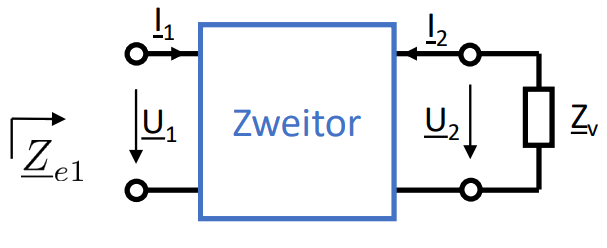
\includegraphics[width=\columnwidth]{Zweipole/Eingangsimpedanz}
\end{minipage}
\begin{minipage}{0.5\columnwidth}
	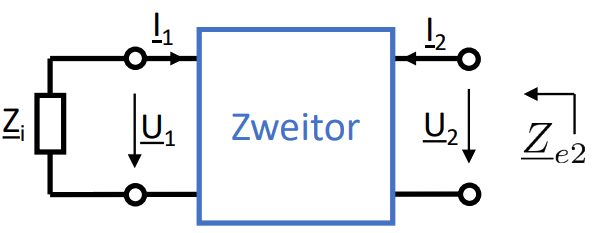
\includegraphics[width=\columnwidth]{Zweipole/Ausgangsimpedanz}
\end{minipage}
	\renewcommand{\arraystretch}{1.8}
\begin{tabularx}{\columnwidth}{|X|l|l|}

	\hline  & Last an Tor 2 & Last an Tor 1 \\
	\hline$Z$ & $ \underline{Z}_{e1} =  \underline{Z}_{11}-\frac{\underline{Z}_{12} \underline{Z}_{21}}{\underline{Z}_{22}+\underline{Z}_{V}}$ & $\underline{Z}_{e 2}=\underline{Z}_{22}-\frac{\underline{Z}_{12} \underline{Z}_{21}}{\underline{Z}_{11}+\underline{Z}_{i}}$ \\
	\hline
	$Y$ & $\underline{Y}_{e 1}=\underline{Y}_{11}-\frac{\underline{Y}_{12} \underline{Y}_{21}}{\underline{Y}_{22}+\underline{Y}_{V}}$ & $\underline{Y}_{e 2}=\underline{Y}_{22}-\frac{\underline{Y}_{12} \underline{Y}_{21}}{\underline{Y}_{11}+\underline{Y}_{i}}$ \\
	\hline
	$A$ & $\underline{Z}_{e 1}=\frac{A_{11} \underline{Z}_{v}+\underline{A}_{12}}{\underline{A}_{21} \underline{Z}_{v}+\underline{A}_{22}}$ & $\underline{Z}_{e 2}=\frac{\underline{A}_{22} \underline{Z}_{i}+\underline{A}_{12}}{\underline{Z}_{21} \underline{Z}_{i}+\underline{A}_{11}}$ \\
	\hline
	$H$ & $\underline{Z}_{e 1}=\underline{H}_{11}-\frac{\underline{H}_{12} \underline{H}_{21}}{\underline{H}_{22}+\underline{Y}_{V}}$ & $\underline{Y}_{e 2}=\underline{H}_{22}-\frac{\underline{H}_{12} \underline{H}_{21}}{\underline{H}_{11}+\underline{Z}_{i}}$ \\
	\hline
	$C$ & $\underline{Y}_{e1}=\underline{C}_{11}-\frac{C_{12} \underline{C}_{21}}{\underline{C}_{22}+\underline{Y}_{V}}$ & $\underline{Z}_{e 2}=\underline{C}_{22}-\frac{\underline{C}_{12} \underline{C}_{21}}{\underline{C}_{11}+\underline{Y}_{i}}$ \\
	\hline
\end{tabularx}

%    \begin{flalign*}
%        \boldsymbol{Z}\rightarrow&\  \underline{Z}_{e1} = \underline{Z}_{11}-\frac{\underline{Z}_{12}\underline{Z}_{21}}{\underline{Z}_{22}+\underline{Z}_V}\\
%        \boldsymbol{Y}\rightarrow&\  \underline{Y}_{e1} = \underline{Y}_{11}-\frac{\underline{Y}_{12}\underline{Y}_{21}}{\underline{Y}_{22}+\underline{Y}_V}\\
%        \boldsymbol{A}\rightarrow&\  \underline{Z}_{e1} = \frac{\underline{A}_{11}\underline{Z}_V + \underline{A}_{12}}{\underline{A}_{21}\underline{Z}_V+\underline{A}_{22}}\\
%        \boldsymbol{H}\rightarrow&\  \underline{Z}_{e1} = \underline{H}_{11}-\frac{\underline{H}_{12}\underline{H}_{21}}{\underline{H}_{22}+\underline{Y}_V}\\
%        \boldsymbol{C}\rightarrow&\  \underline{Y}_{e1} = \underline{C}_{11}-\frac{\underline{C}_{12}\underline{C}_{21}}{\underline{C}_{22}+\underline{Z}_V}\\
%    \end{flalign*}
%\raggedright
%
%\subsubsection{Ausgangsimpedanz}
%\centering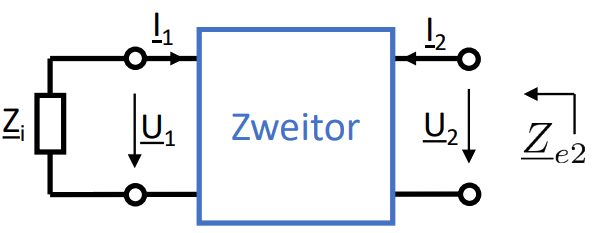
\includegraphics[width=0.5\columnwidth]{Zweipole/Ausgangsimpedanz}
%\begin{mdframed}[style=exercise]
%    \begin{align*}
%        \boldsymbol{Z}\rightarrow&\  \underline{Z}_{e2} = \underline{Z}_{22}-\frac{\underline{Z}_{12}\underline{Z}_{21}}{\underline{Z}_{11}+\underline{Z}_i}\\
%        \boldsymbol{Y}\rightarrow&\  \underline{Y}_{e2} = \underline{Y}_{22}-\frac{\underline{Y}_{12}\underline{Y}_{21}}{\underline{Y}_{11}+\underline{Y}_i}\\
%        \boldsymbol{A}\rightarrow&\  \underline{Z}_{e2} = \frac{\underline{A}_{22}\underline{Z}_i + \underline{A}_{12}}{\underline{A}_{21}\underline{Z}_i+\underline{A}_{11}}\\
%        \boldsymbol{H}\rightarrow&\  \underline{Z}_{e2} = \underline{H}_{22}-\frac{\underline{H}_{12}\underline{H}_{21}}{\underline{H}_{11}+\underline{Y}_i}\\
%        \boldsymbol{C}\rightarrow&\  \underline{Y}_{e2} = \underline{C}_{22}-\frac{\underline{C}_{12}\underline{C}_{21}}{\underline{C}_{11}+\underline{Z}_i}\\
%    \end{align*}
%\end{mdframed}
%\raggedright

\subsubsection{Ersatzquelle}
Berechnung Innenwiderstand $\underline{Z}_i$ eines Ersatz-Zweipols:\\ 
Quellen $U_q$ kurzschließen. $I_q$ unterbrechen.\\
Gilt nicht bei gesteuerten Quellen.\\
\begin{center}
	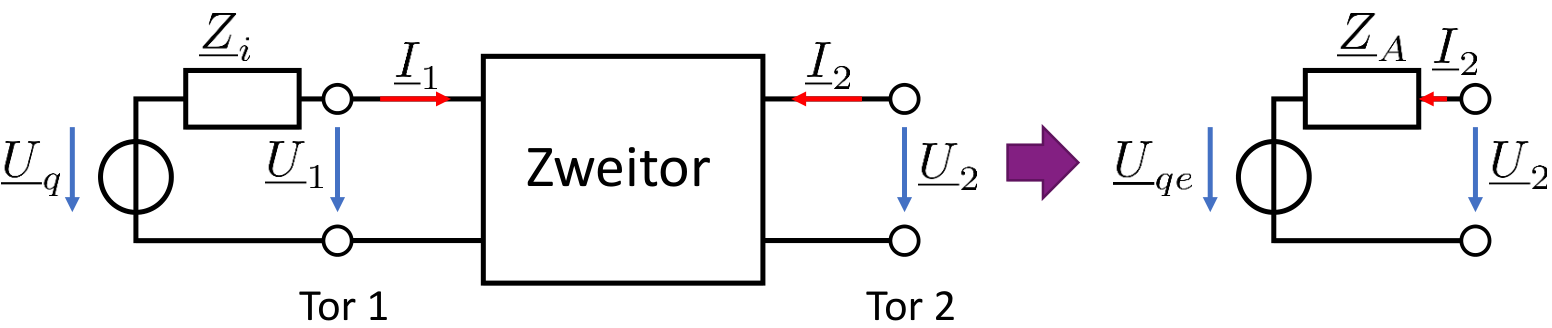
\includegraphics[width=\columnwidth]{Zweipole/Ersatzquelle_2}
\end{center}
\begin{tabularx}{\columnwidth}{|c|X|X|}
	\hline
	 & Quelle an Tor 1 & Quelle an Tor 2 \\
	\hline A & $\underline{U}_{q e}=\frac{1}{\underline{A}_{21} \underline{Z}_i+\underline{A}_{11}} \underline{U}_q$ & $\underline{U}_{q e}=\frac{\operatorname{det}(\underline{A})}{\underline{A}_{21} \underline{Z}_i+\underline{A}_{22}} \underline{U}_q$ \\
	\hline Z & $\underline{U}_{q e}=\frac{\underline{Z}_{21}}{\underline{Z}_{11}+\underline{Z}_i} \underline{U}_q$ & $\underline{U}_{q e}=\frac{\underline{Z}_{12}}{\underline{Z}_{22}+\underline{Z}_i} \underline{U}_q$ \\
	\hline Y & $\underline{I}_{q e}=-\frac{\underline{Y}_{21}}{\underline{Y}_{11}+\underline{Y}_i} \underline{I}_q$ & $\underline{I}_{q e}=-\frac{\underline{Y}_{12}}{\underline{Y}_{22}+\underline{Y}_i} \underline{I}_q$ \\
	\hline H & $\underline{I}_{q e}=-\frac{\underline{H}_{21}}{\underline{H}_{11}+\underline{Z}_i} \underline{U}_q$ & $\underline{U}_{q e}=\frac{\underline{H}_{12}}{\underline{H}_{22}+\underline{Y}_i} \underline{I}_q$ \\
	\hline
\end{tabularx}
\begin{tabularx}{\columnwidth}{|c|X|X|}
	\hline
	        & Quelle an Tor 1 & Quelle an Tor 2 \\
	\hline
	A & $Z_A = \frac{A_{22}Z_i + A_{12}}{A_{21}Z_i + A_{11}}$ & $Z_A = \frac{A_{11}Z_i + A_{12}}{A_{21}Z_i + A_{22}}$ \\
	\hline
	Z & $Z_A = Z_{22} - \frac{Z_{12} Z_{21}}{Z_{11} + Z_i}$ & $Z_A = Z_{11} - \frac{Z_{12} Z_{21}}{Z_{22} + Z_i}$ \\
	\hline
	Y & $Y_A = Y_{22} - \frac{Y_{12} Y_{21}}{Y_{11} + Y_i}$ & $Y_A = Y_{11} - \frac{Y_{12} Y_{21}}{Y_{22} + Y_i}$ \\
	\hline
	H & $Y_A = H_{22} - \frac{H_{12} H_{21}}{H_{11} + Z_i}$ & $Z_A = H_{11} - \frac{H_{12} H_{21}}{H_{22} + Y_i}$ \\
	\hline
\end{tabularx}
siehe Ausgangsimpedanz $Z_{e2} = Z_A$ (Quelle an Tor 1).

\subsubsection{Wellenwiderstand}
\begin{minipage}{0.5\columnwidth}
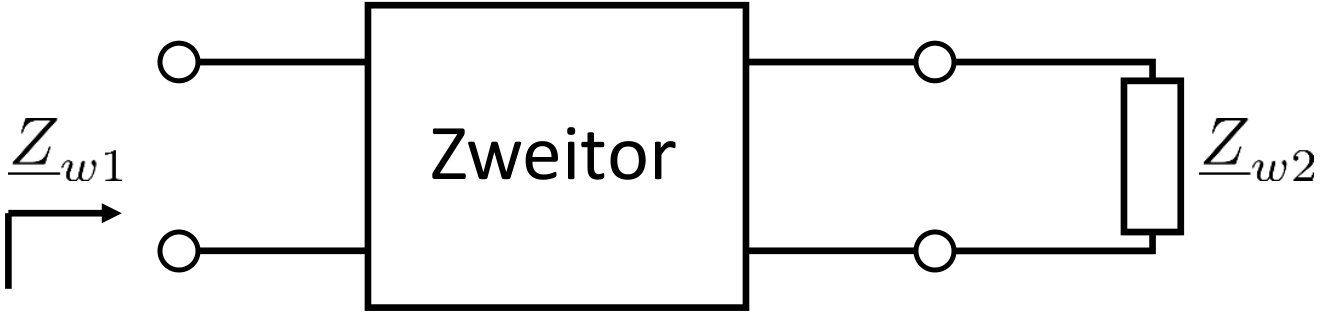
\includegraphics[width=\columnwidth]{Zweipole/wellenwiderstand_an_tor_2}
\end{minipage}
\begin{minipage}{0.5\columnwidth}
	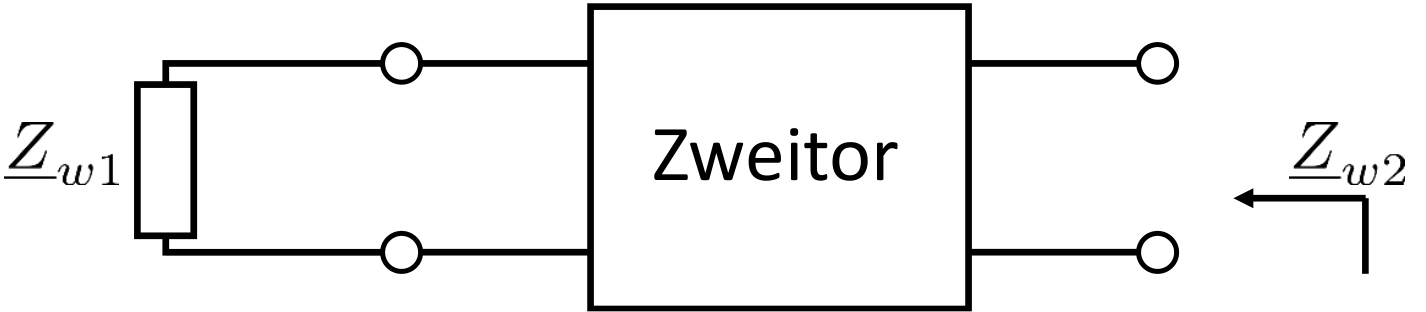
\includegraphics[width=\columnwidth]{Zweipole/wellenwiderstand_an_tor_1}
\end{minipage}
\begin{gather*}
	\boxed{
	\underline{Z}_{w1} = \frac{\underline{A}_{11}\underline{Z}_{w2} + \underline{A}_{12}}{\underline{A}_{21}\underline{Z}_{w2}+\underline{A}_{22}}
	} \qquad \boxed{
  	\underline{Z}_{w2} = \frac{\underline{A}_{22}\underline{Z}_{w1} + \underline{A}_{12}}{\underline{A}_{21}\underline{Z}_{w1}+\underline{A}_{11}}
  	}
\end{gather*}
\begin{minipage}{0.5\columnwidth}
\renewcommand{\arraystretch}{2}
	symmetrische ZT: $\underline{Z}_{w1}=\underline{Z}_{w2}$\\
	\begin{tabular}{|c|c|c|}
		\hline
		& $\boldsymbol{\underline{Z}_{w1}}$ & $\boldsymbol{\underline{Z}_{w2}}$
		\\
		\hline
		$\underline{\boldsymbol{Z}}$ & $\sqrt{\frac{\underline{Z}_{11}\operatorname{det}\underline{Z}}{\underline{Z}_{22}}}$ & $\sqrt{\frac{\underline{Z}_{22}\operatorname{det}\underline{Z}}{\underline{Z}_{11}}}$
		\\
		\hline
		$\underline{\boldsymbol{Y}}$ & $\sqrt{\frac{\underline{Y}_{22}}{\underline{Y}_{11}\operatorname{det}\underline{Y}}}$ & $\sqrt{\frac{\underline{Y}_{11}}{\underline{Y}_{22}\operatorname{det}\underline{Y}}}$
		\\
		\hline
		$\underline{\boldsymbol{A}}$ & $\sqrt{\frac{\underline{A}_{11}\cdot\underline{A}_{12}}{\underline{A}_{21}\cdot\underline{A}_{22}}}$ & $\sqrt{\frac{\underline{A}_{22}\cdot\underline{A}_{12}}{\underline{A}_{21}\cdot\underline{A}_{11}}}$
		\\
		\hline
		$\underline{\boldsymbol{H}}$ & $\sqrt{\frac{\underline{H}_{11}\operatorname{det}\underline{H}}{\underline{H}_{22}}}$ & $\sqrt{\frac{\underline{H}_{11}}{\underline{H}_{22}\operatorname{det}\underline{H}}}$
		\\
		\hline
		$\underline{\boldsymbol{C}}$ & $\sqrt{\frac{\underline{C}_{22}}{\underline{C}_{11}\operatorname{det}\underline{C}}}$ & $\sqrt{\frac{\underline{C}_{11}\operatorname{det}\underline{C}}{\underline{C}_{11}}}$
		\\
		\hline
	\end{tabular}
\end{minipage}
\begin{minipage}{0.5\columnwidth}
	\small
	\begin{itemize}
	\item Messtechnische\\ Ermittlung:
	
	$Z_{01}$: Leerlauf - Tor 1\\
	$Z_{k1}$: Kurzschluss - Tor 1
	\end{itemize}

	\begin{align*}
		\underline{Z}_{w1} &= \sqrt{\underline{Z}_{k1}\cdot\underline{Z}_{01}}\\
		&=\sqrt{\frac{\underline{A}_{11}\cdot\underline{A}_{12}}{\underline{A}_{21}\cdot\underline{A}_{22}}}
	\end{align*}
\end{minipage}

    
\subsubsection{Scheinleistungsanpassung}
\begin{minipage}{0.55\columnwidth}
	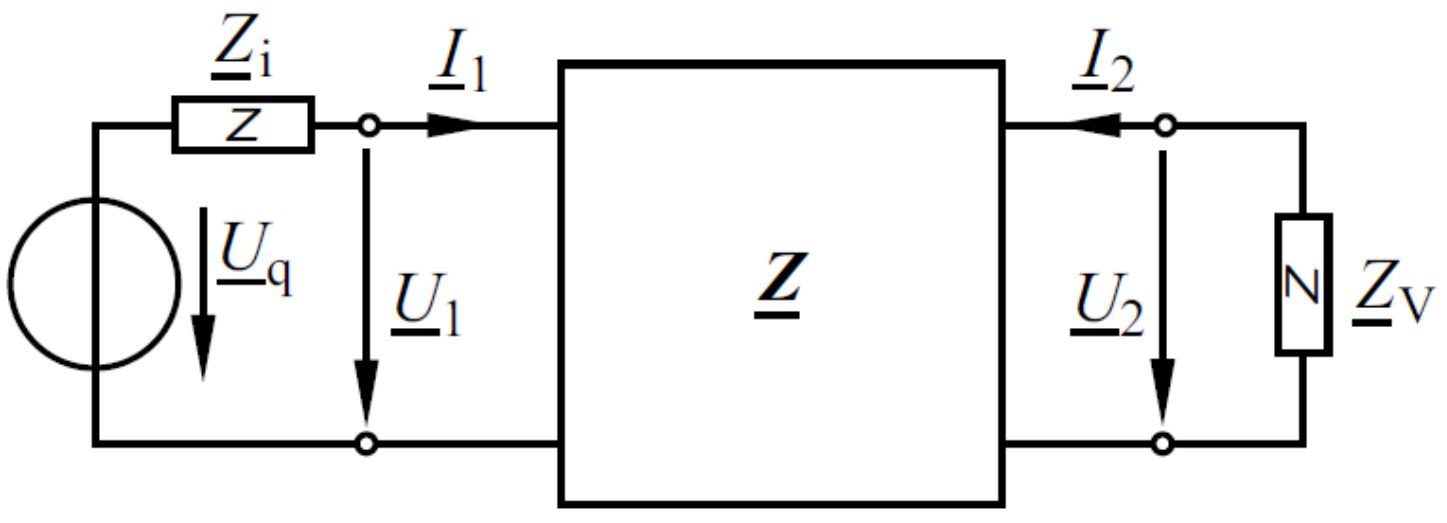
\includegraphics[width=\columnwidth]{Zweipole/scheinleistungsanpassung}
\end{minipage}
\begin{minipage}{0.45\columnwidth}
$\quad \underline{Z}_i = \underline{Z}_{w1} \quad \underline{Z}_V=\underline{Z}_{w2}
$
\end{minipage}

Beschaltet man jedes Tor mit seinem Wellenwiderstand, so liegt Scheinleistungsanpassung vor.

\subsubsection{Kettenwiderstand}
\begin{minipage}{0.5\columnwidth}
	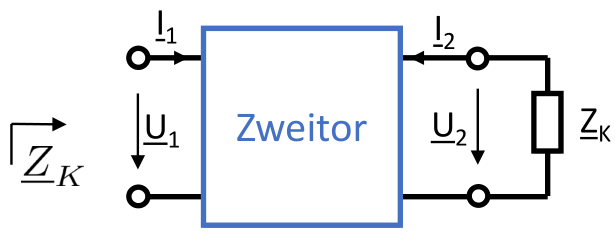
\includegraphics[width=\columnwidth]{Zweipole/Kettenwiderstand}
\end{minipage}
\begin{minipage}[b]{0.5\columnwidth}
	$$
	\underline{Z}_K = \underline{Z}_{11} - \frac{\underline{Z}_{12}\underline{Z}_{21}}{\underline{Z}_{22}+\underline{Z}_K}
	$$
\end{minipage}
\\
\small
Schaltet man eine große Zahl gleicher Zweitore in Kette, so nähert sich der
Eingangswiderstand dem Kettenwiderstand $\mathbf{\underline{Z}_K}$ an.\\
L\"osung der obigen Gleichung:
\[
    \underline{Z}_K = \frac{1}{2}(\underline{Z}_{11} - \underline{Z}_{22} \pm \sqrt{(\underline{Z}_{11}-\underline{Z}_{22})^2+4\cdot\operatorname{det}\underline{Z}})
\]
Symmetrische ZT: Kettenwiderstand = Wellenwiderstand.
\normalsize

\section{Signaldarstellung im Frequenz- und Bildbereich}
\subsection{Fourierreihe periodischer Signale}
Die Überlagerung von Sinusschwingungen zu einem periodischen,
nichtsinusförmigen Signal nennt man harmonische Synthese.
\subsubsection{Reelle Fourierreihe}
\begin{mdframed}[style=exercise]
	\begin{itemize}
		\item mit $sin$ und $cos$:
		      \[
			      f(t) = a_0 \sum_{k=1}^\infty [a_k\cdot cos(k\omega_1 t) b_k\cdot sin(k\omega_1 t)]
		      \]
		\item mit Amplitude und Phase:
		      \begin{align*}
			      f(t) & = A_0+\sum_{k=1}^\infty [A_k\cdot cos(k\omega_1 t + \varphi_k)]               \\
			           & = A_0+\sum_{k=1}^\infty [A_k\cdot sin(k\omega_1 t + \varphi_k-\frac{\pi}{2})]
		      \end{align*}

		      \texttt{\footnotesize Koeffizienten }
		      \[
			      A_0 = \frac{1}{T}\int_{t_0}^{T+t_0} f(t)dt
		      \]
		      \begin{align*}
			      a_k = \frac{2}{T}\int_{t_0}^{T+t_0} f(t)\cdot cos(k\omega_1 t) dt \\
			      b_k = \frac{2}{T}\int_{t_0}^{T+t_0} f(t)\cdot sin(k\omega_1 t) dt
		      \end{align*}
	\end{itemize}
\end{mdframed}

\subsubsection{Komplexe Fourierreihe}
\begin{mdframed}[style=exercise]
	\[
		f(t)=\sum_{k=-\infty}^{\infty} \underline{c}_k\cdot e^{j\omega_1 k t}
	\]
	\begin{align*}
		\underline{c}_k & = \frac{1}{T}\int_{t_0}^{T+t_0} f(t)\cdot e^{-j\omega_1 k t}dt
		                & = \frac{1}{2}\left( a_k-jb_k \right)
	\end{align*}
\end{mdframed}

\subsubsection{Komplex Reell umwandeln}
\begin{mdframed}[style=exercise]
	\begin{gather*}
		\texttt{\footnotesize Komplex $\rightarrow$ Reell:}\\
		a_0 = A_0 = \underline{c}_0\\
		\left.
		\begin{split}
			a_k = 2\ \mathfrak{Re}\left\{ c_k \right\}= \left[ \underline{c}_k+\underline{c}_{-k} \right]\\
			b_k = -2\ \mathfrak{Im}\left\{ \underline{c}_k \right\}= j\left[ \underline{c}_k-\underline{c}_{-k} \right]\\
			A_k = 2|\underline{c}_k| \quad \beta_k = -\varphi_k
		\end{split}\right\} \quad k>0\\
		\texttt{\footnotesize Reell $\rightarrow$ Komplex:}\\
		\left.
		\begin{split}
			\underline{c}_k = \frac{1}{2}\left( a_k-jb_k \right) = \frac{A_k}{2} e^{-j\beta_k}\\
			\underline{c}_{-k} = \frac{1}{2}\left( a_k+jb_k \right) = \frac{A_k}{2} e^{j\beta_k}
		\end{split}\right\} \quad k>0\\
	\end{gather*}
\end{mdframed}

\subsubsection{Symmetrieeigenschaften}
\begin{itemize}
	\item Gerade Funktionen
	      symmetrisch zur y-Achse\\
	      alle $sin$-teile verschwinden
	      - $A_0 = \frac{2}{T}\int^{\frac{T}{2}}_{0} y(t)dt$\\
	      - $a_{k} = \frac{4}{T}\int^{\frac{T}{2}}_{0}y(t)\cdot cos(k\omega_1t)dt$\\
	      - $b_k = 0$\\
	\item Ungerade Funktionen
	      symmetrisch zum Ursprung\\
	      alle $cos$-teile und Gleichanteil verschwinden

	      - $A_0 = 0$\\
	      - $a_k = 0$\\
	      - $b_{k} = \frac{4}{T}\int^{\frac{T}{2}}_{0} y(t)\cdot sin(k\omega_1t)dt$\\
\end{itemize}
\subsubsection{Halbwellensymmetrie}
Halbwellensymmetrie gilt wenn:
\[
	y(t) = -y(t \pm T/2)
\]
Die Fourier-Reihe einer Zeitfunktion mit HWS enthält stets
nur Terme mit ungeraden Ordnungszahlen. $k=1,3,5,\dots,\infty$
\begin{mdframed}[style=exercise,frametitle=im Allgemeinen]
	\texttt{\footnotesize Koeffizienten}:\\
	\[
		A_0 = 0,\
		a_{2k} = 0,\
		b_{2k} = 0
	\]
	$$a_{2k-1} = \frac{4}{T}\int^{\frac{T}{2}}_{0}y(t)\cdot cos((2k-1)\omega_1t)dt$$
	$$b_{2k-1} = \frac{4}{T}\int^{\frac{T}{2}}_{0}y(t)\cdot sin((2k-1)\omega_1t)dt$$
\end{mdframed}
\begin{mdframed}[style=exercise,frametitle=gerade Halbwellensymmetrie]
	\[
		A_0 = 0,\
		b_k = 0,\
		a_{2k} = 0
	\]
	$$a_{2k-1} = \frac{8}{T}\int^{\frac{T}{4}}_{0}y(t)\cdot cos((2k-1)\omega_1t)dt$$
\end{mdframed}
\begin{mdframed}[style=exercise,frametitle=ungerade Halbwellensymmetrie]
	\[
		A_0 = 0,\
		a_k = 0,\
		b_{2k} = 0
	\]
	$$b_{2k-1} = \frac{8}{T}\int^{\frac{T}{4}}_{0}y(t)\cdot sin((2k-1)\omega_1t)dt$$
\end{mdframed}

\subsubsection{Verschiebungssatz}
Verschiebung im Zeitbereich entspricht eine Drehung den Komplexen Spektrum um
die Phase $\rightarrow\ -k\omega_1 t_v$
\begin{align*}
	f_v(t) = f(t-t_v) & = \sum_{k=-\infty}^{\infty} \underline{c}_k\cdot e^{j\omega_1 k (t-t_v)}                                                       \\
	                  & = \sum_{k=-\infty}^{\infty} \underbrace{\underline{c}_k\cdot e^{j\omega_1 k t_v}}_{\underline{c}_{k_v}} \cdot e^{\omega_1 k t}
\end{align*}

Ist tv < 0, wie im Beispiel oben, so werden die Phasenwinkel des Spektrums mit
zunehmender Frequenz größer.

\subsubsection{Fourierreihe und LTI-Systeme}

\[
	y(t) = \sum_{k=-\infty}^{\infty} \underbrace{\underline{H}(k\omega_1)\cdot\underline{c}_{xk}}_{\underline{c}_{yk}} \cdot e^{j\omega_1 k t}
\]

\subsection{Kenngrößen periodischer Signale}
\begin{itemize}
	\item Effektivwert
	      \[
		      \boxed{U_{\mathit{eff}} = \sqrt{\frac{1}{T} \int_\tau^{\tau+T} u(t)^2 dt}}
	      \]
	      \begin{mdframed}[style=exercise]
		      mit der Fourierreihe:
		      $$ U_{\mathit{eff}} = \sqrt{\sum_{k=-\infty}^{\infty} c_k^2} = \sqrt{\sum_{k=-\infty}^{\infty}U_{k,\mathit{eff}}^2} $$
		      auch:
		      $$ \sqrt{A_0^2 + \frac{1}{2} \sum_{k=1}^{\infty} A_k^2} $$
	      \end{mdframed}
	\item Klirrfaktor(Oberschwingungsgehalt):\\
	      Dient zur Quantifizierung einer nichtlinearen Verzerrung bzw. von der
	      Sinusform eines Signals.
	      \begin{align*}
		      k & = \frac{\text{Effektivwert der Oberschwingungen}}{\text{Effektivwert des Wechselanteil}}                                                                                  \\
		        & = \boxed{\frac{\sqrt{\sum_{{\color{red}{k=2}}}^{\infty} U_{k}^{2}}}{\sqrt{\sum_{{\color{red}{k=1}}}^{\infty} U_{k}^{2}}} = \frac{\sqrt{U_\sim^2 - U_1^2}}{U_\sim} \leq 1}
	      \end{align*}
	      Für Wechselgrößen lässt sich $k$ einfach mit \textbf{Grundschwingungsgehalt} $g$ ermitteln (\textit{gilt immer}):
	      \[
		      \boxed{k = \sqrt{1-g^2} \leftrightarrow g = \frac{U_1}{U}}
	      \]
	\item Mischgrößen\\
	      - Schwingungsgehalt:
	      \[
		      s = \frac{U_\sim}{U} = \frac{\textsc{Effektivwert des Wechselanteils}}{\textsc{Effektivwert der Mischgröße}}
	      \]
	      - Welligkeit:
	      \[
		      w = \frac{U_\sim}{\bar{U}} = \frac{\textsc{Effektivwert des Wechselanteils}}{\textsc{Gleichanteil}}
	      \]
	      - Riffelfaktor:
	      \[
		      R = \frac{\hat{U}_\sim}{\bar{U}} = \frac{\textsc{Scheitelwert des Wechselanteils}}{\textsc{Gleichanteil}}
	      \]
	\item Wirkleistung:
	      \[
		      P = \bar{p}(t) = \frac{1}{T} \int_0^T u(t)\cdot i(t) dt
	      \]
	      \[
		      P = \sum_{k=-\infty}^{\infty}\underline{u}_k \underline{i}_k^* \leftrightarrow i_k^* = i_{-k}
	      \]
	      \begin{mdframed}[style=exercise]
		      Als Reihe:
		      \[
			      P_0 + \sum_{k=1}^{\infty} U_{k_{\mathit{eff}}}\cdot
			      I_{k_{\mathit{eff}}}\cdot\cos(\varphi_{uk}-\varphi_{ik}) = \sum_{k=0}^{\infty}P_k
		      \]
	      \end{mdframed}
	      Nur gleichfrequente harmonische tragen zur Wirkleistung bei!
	\item Schein- und Blindleistung\\
	      \vspace{-0.5em}
	      \[
		      \boxed{S = U_{\mathit{eff}}\cdot I_{\mathit{eff}} = U\cdot I = \sqrt{P^2+Q^2}}
	      \]
	      \vspace{-0.5em}
	      \begin{mdframed}[style=exercise]
		      Bei einem nicht linearen Verbraucher an einer Sinusförmigen Spannung:
		      \vspace{-1em}
		      \begin{multline*}
			      S^{2}=(U I)^{2}=U_{1}^{2} \cdot \sum_{k=0}^{\infty} I_{k}^{2}=\\U_{1}^{2} I_{0}^{2}+U_{1}^{2} \sum_{k=2}^{\infty} I_{k}^{2}+U_{1}^{2} I_{1}^{2} \sin ^{2} \varphi_{1}+U_{1}^{2} I_{1}^{2} \cos ^{2} \varphi_{1}
		      \end{multline*}
	      \end{mdframed}

	      Räumlich Darstellung der Scheinleistung:
	      \begin{center}
		      \vspace{-0.5em}
		      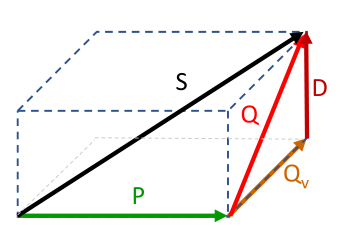
\includegraphics[width=0.35\columnwidth]{Schein-Blindleistung_raeumlich.png}
		      \vspace{-0.6em}
	      \end{center}

	      \begin{mdframed}[style=exercise,frametitle=Verschiebungs- Feldblindleistung $Q_v$]
		      \vspace{-1em}
		      \begin{gather*}
			      Q = \sqrt{Q^2_v + D^2} \leftrightarrow Q = \sqrt{S^2-P^2}\\
			      S = \sqrt{P^2+Q^2_v + D^2}
		      \end{gather*}
		      Blindleistung aufgrund der Phasenverschiebung zwischen Strom und
		      Spannung gleicher Frequenz.
	      \end{mdframed}

	      \begin{mdframed}[style=exercise,frametitle=Verzerrungblindleistun $D$]
		      \[
			      D^2 = U_1^2\cdot(I^2-I_1^2) = S^2(1-g)
		      \]
		      von Mischtermen (Produkten von Spannung und Strom unterschiedlicher
		      Frequenzen).
	      \end{mdframed}
\end{itemize}

\subsection{Fouriertransformation}
\begin{mdframed}[style=exercise]
	\[
		x(t) \laplace X(\omega)
	\]
	Hintransformation - Analysegleichung:
	\[
		\underline{X}(\omega)=\mathcal{F}\left\{ x(t) \right\} = \int_{-\infty}^{\infty} x(t) \cdot e^{-j\omega t} dt
	\]
	Komplexwertige Fouriertransformierte:
	\[
		\underline{X}(\omega) = |\underline{X}(\omega)|\cdot e^{j\omega\varphi}
	\]
	\footnotesize
	$$\textsc{Einheit:} \left[ x(t) \right]\cdot s$$

	\normalsize

	Rücktransformation - Synthesegleichung:
	\[
		x(t) = \mathcal{F}^{-1}\left\{ \underline{X}(\omega) \right\} = \frac{1}{2\pi}\int_{-\infty}^{\infty} \underline{X}(\omega) \cdot e^{j\omega t} d\omega
	\]
\end{mdframed}

\subsection{Fouriertransformation bei periodischer Signale}
\begin{mdframed}[style=exercise]

	Fouriertransformierte periodischer Signale:
	\[
		\quad \underline{X}(\omega) =
		2\pi\sum_{k=-\infty}^{\infty} \underline{c}_k\cdot
		\delta(\omega-k\omega_1)
	\]

	Fourierkoeffizienten:
	\[
		\quad \underline{c}_k =
		\frac{1}{T}\underline{X}(\omega_1) =
		\frac{1}{T}\int_0^T x(t) \cdot e^{-j\omega_1 t} dt
	\]

	Die Koeffizienten $\underline{c}_k $ der komplexen Fourierreihe sind die
	Abtastwerte von $\underline{X}(\omega)$ bei den Frequenzen
	\[\omega=k\omega_1=k\frac{2\pi}{T}\]
\end{mdframed}

\subsection{Eigenschaften der Fouriertransformation}
\begin{mdframed}[style=exercise,nobreak=false]
	\begin{itemize}
		\item \textbf{Linearität}
		      \[
			      a_{1} x_{1}(t)+a_{2} x_{2}(t)\ \laplace\  a_{1} \underline{X}_{1}(\omega)+a_{2} \underline{X}_{2}(\omega)
		      \]
		      % {\footnotesize Eine lineare Überlagerung von gewichteten Zeitsignalen führt zur linearen
		      % Überlagerung der Spektren mit denselben Vorfaktoren.}
		\item \textbf{Dualität}
		      \[
			      \underline{X}(t)\ \laplace\  2\pi\cdot x(-\omega)
		      \]
		      % {\footnotesize Zeit- und Frequenzbereich können vertauscht werden (bis auf den Faktor $2\pi$
		      % und einer Vorzeichenumkehr).}
		\item \textbf{Zeitskalierung}
		      \[
			      x(a \cdot t)\ \laplace\ \frac{1}{|a|} \underline{X}\left(\frac{\omega}{a}\right) \quad a \in \mathbb{R} \backslash\{0\}
		      \]
		      % {\footnotesize Eine Stauchung der Zeitachse führt zur Dehnung der Frequenzachse.
		      % Frequenzachse (und Skalierung der Amplitude).}
		\item \textbf{Frequenzskalierung}
		      \[
			      \frac{1}{|b|} x\left(\frac{t}{b}\right)\ \laplace\ \underline{X}(b\cdot\omega) \quad b \in \mathbb{R} \backslash\{0\}
		      \]
		      % {\footnotesize Eine Stauchung der Frequenzachse führt zur Dehnung der Zeitachse.
		      % Zeitachse (und Skalierung der Amplitude).}
		\item \textbf{Zeitverschiebung}
		      \[
			      x\left(t-t_{0}\right)\ \laplace\ \underline{X}(\omega) \cdot e^{-j \omega t_{0}}
		      \]
		      % {\footnotesize Eine Verschiebung im Zeitbereich ändert nicht den Betrag des Spektrums,
		      % aber die Phase um einen sich mit der Frequenz $\omega$ linear ändernden Phasenterm.}
		\item \textbf{Frequenzverschiebung - Modulation}
		      \[
			      x(t) \cdot e^{j \omega_{0} t}\ \laplace\ \underline{X}\left(\omega-\omega_{0}\right)
		      \]
		      % {\footnotesize Eine Verschiebung im Frequenzbereich führt zu einem Modulationsterm im
		      % Zeitbereich oder andersherum, um eine Frequenzverschiebung zu erreichen,
		      % muss im Zeitbereich mit $e^{(j\omega_0t)}$ multipliziert (moduliert) werden.}
		\item \textbf{Faltungssatz}
		      \[
			      x_{1}(t) * x_{2}(t)\ \laplace\ \underline{X}_{1}(\omega) \cdot \underline{X}_{2}(\omega)
		      \]
		      % {\footnotesize Faltung im Zeitbereich entspricht Multiplikation im Frequenzbereich}
		\item \textbf{Multiplikation - Fenstertheorem}
		      \[
			      x_{1}(t) \cdot x_{2}(t)\ \laplace\ \frac{1}{2 \pi} \underline{X}_{1}(\omega) * \underline{X}_{2}(\omega)
		      \]
		      % {\footnotesize Multiplikation im Zeitbereich entspricht Faltung im Frequenzbereich (und
		      % Normierung mit $2\pi$).}
		\item \textbf{Differentiation\\}
		      {\small im Zeitbereich:}
		      \[
			      \frac{d}{dt} x(t) \ \laplace\ j\omega\underline{X}(\omega)
		      \]
		      {\small im Frequenzbereich:}
		      \[
			      t \cdot x(t)\ \laplace\ j \frac{d}{d \omega} \underline{X}(\omega)
		      \]
		      % {\footnotesize Differenzieren im Zeitbereich dreht die Phase des Spektrums um $\frac{\pi}{2}$ und
		      % verstärkt die Amplitude des Spektrums zu hohen Frequenzen hin mit linear
		      % anwachsendem $\omega$.}
		\item \textbf{Integration}
		      \[
			      \int_{-\infty}^{t} x(\tau) d \tau\ \laplace\ \frac{1}{j \omega} \underline{X}(\omega)+\pi \cdot \underline{X}(0) \cdot \delta(\omega)
		      \]
		      % {\footnotesize Integrieren dreht die Phase um $-\frac{\pi}{2}$, dämpft die Amplitude des
		      % Spektrums mit $\frac{1}{\omega}$ und erzeugt einen (dem Gleichanteil von
		      % $x(t)$ entsprechenden) Dirac bei $\omega = 0$.}
		\item \textbf{Energieberechnung - Parseval}
		      \[
			      \int_{-\infty}^{+\infty}|x(t)|^{2} d t=\frac{1}{2 \pi} \int_{-\infty}^{+\infty}|\underline{X}(\omega)|^{2} d \omega
		      \]
		      % {\footnotesize Die Signalenergie lässt sich aus der Zeit- und Frequenzbereichsdarstellung berechnen.}
	\end{itemize}
\end{mdframed}
\begin{mdframed}[style=exercise,frametitle=Symmetrie,nobreak=true]
	\begin{wrapfigure}[10]{R}{0.27\textwidth}
		\vspace{-1.4em}
		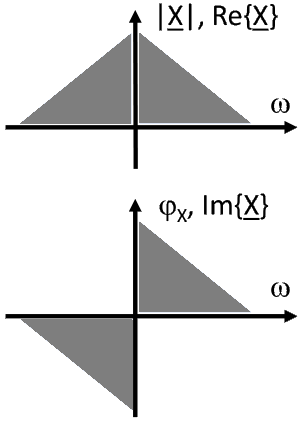
\includegraphics[width=0.3\textwidth]{FT_Symmetrie.png}
	\end{wrapfigure}

	\begin{minipage}{5cm}
		Betrag und der Realteil des Spektrums sind gerade\\
	\end{minipage}

	\begin{minipage}{5cm}
		Phase und der Imaginärteil des Spektrums sind ungerade.
	\end{minipage}

	\[
		\underline{X}(-\omega) = \underline{X}^*(\omega)
	\]

	\begin{gather*}
		x(t)\text{ reel und gerade}\rightarrow X(\omega)\text{ reel und gerade}\\
		\underline{X}(\omega) = 2\int_0^\infty x(t)\cos(\omega t)dt\\
		x(t)\text{ reel und ungerade}\rightarrow X(\omega)\text{ imaginär und ungerade}\\
		\underline{X}(\omega) = -2j\int_0^\infty x(t)\sin(\omega t)dt
	\end{gather*}
\end{mdframed}
\newpage

\section{Laplace-Transformation (LPT)}
	Hintransformation - Analyse:
	\[
		 \mathcal{L}\left\{ x(t) \right\} = \boxed{ \underline{X}(s) = \int_0^\infty x(t) \cdot e^{-st} dt }
	\]
	Rücktransformation - Synthese:
	\[
		 \mathcal{L}^{-1}\left\{ \underline{X}(s) \right\} = x(t) =  \frac{1}{2\pi j}\int_{\sigma-j\infty}^{\sigma+j\infty} \underline{X}(s) \cdot e^{-st} ds
	\]
Rücktransformation mit Partialbruchzerlegung (PBZ) + Tabelle in Kap. \ref{lpt_tabelle}.

\normalsize
\subsection{LTI-Systeme im Bildbereich (BB)}
$x(t)=h(t)=0$ für $t<0$: Rechtsseitige (\textbf{kausale}) Signale!
\begin{center}
	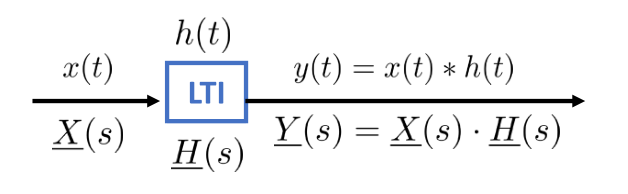
\includegraphics[width=0.6\columnwidth]{Bilder/LTI_Systeme_im_Bildbereich.png}
\end{center}
LTI-Systeme im Bildbereich sind \textbf{immer} kausal!

\subsection{Impuls- und Sprungantwort im BB}
Impulsantwort:
\[
h(t)\ \laplace\ \underline{H}(s)
\]
Sprungantwort:
\[
g(t) = \int_0^t h(\tau) d\tau \quad \laplace\ \quad \boxed{\underline{G}(s) = \frac{\underline{H}(s)}{s}}
\]

\subsection{P/N-Diagramm: Systemeigenschaften}\label{pn_diagramm_lpt}
\begin{itemize}
	\item \textbf{Stabilität}: \textbf{Alle} Pole von $\underline{H}(s)$ liegen links der\\ $\omega$-Achse.
	\item \textbf{Minimalphasiges} System: \textbf{Alle} Nullstellen liegen links der $\omega$-Achse.
\end{itemize}

\subsubsection{Zusammenhang LPT $\leftrightarrow$ FT}
Weitere Infos siehe Kap. \ref{fgang_pn}.
\begin{itemize}
	\item Konvergenzbereich (Kb): Halbebene rechts vom am \underline{weitesten} rechts liegenden Pol.
	\item Wenn $\omega$-Achse $\in$ Kb, dann \underline{existiert} eine FT von $\underline{X}(s)$:
	\[
	\mathcal{F}\{x(t)\} = X(\omega) = X(s) \big|_{s=j\omega} = \mathcal{L}\{x(t)\} \big|_{s=j\omega}
	\]
	$\Rightarrow$ Wenn System instabil, dann gibt es keine FT!
\end{itemize}
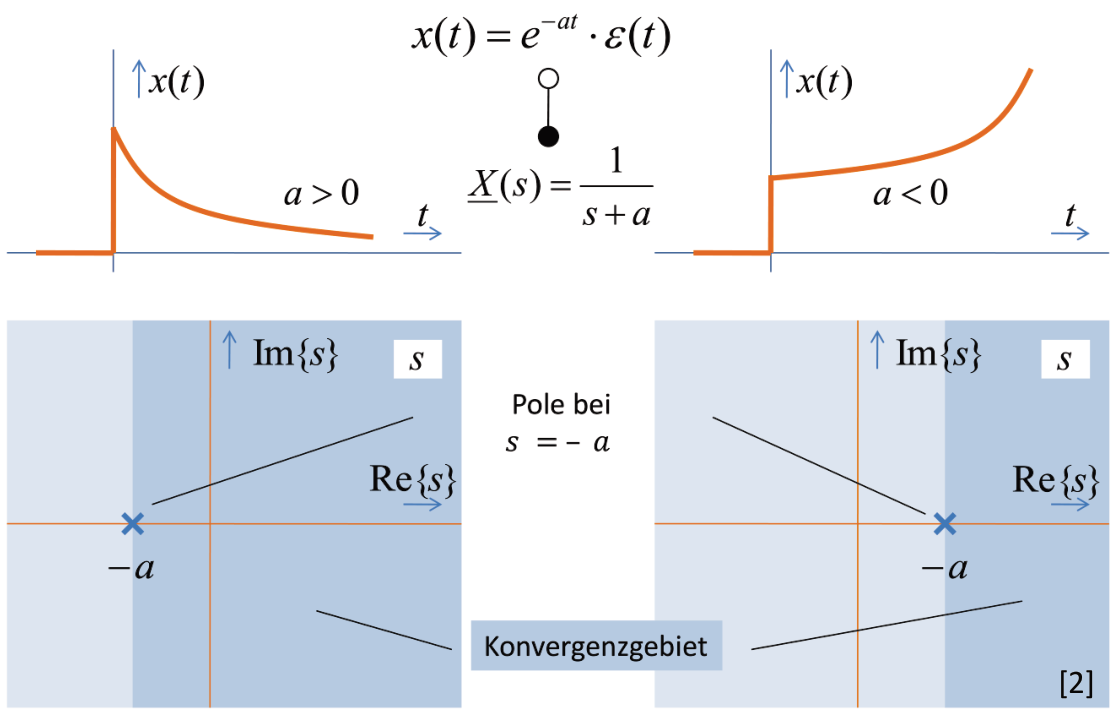
\includegraphics[width=\columnwidth]{zusammenhang_ft_lpt}
\subsection{Partialbruchzerlegung (PBZ)}
Für die inverse bzw. Rücktransformation in den Zeitbereich. Beispiele siehe Papula FS. S.157f.
\begin{itemize}
	\item Einfache Polstellen:
		\begin{align*}
		\underline{X}(s) &= \frac{\underline{Z}(s)}{\underline{N}(s)} = \sum_{n=1}^{N} \frac{A_n}{(s - p_n)}
	\end{align*}
	\item Doppelte/k-fache Polstellen:
	\begin{align*}
			\underline{X}(s) &= \frac{\underline{Z}(s)}{\underline{N}(s)} = \frac{\underline{Z}(s)}{(s - p_n)^k} \\
			&= \frac{A_1}{s - p_{n}} + \frac{A_2}{(s - p_{n})^2} + \cdots + \frac{A_k}{(s - p_{n})^k}
	\end{align*}
	\item \textbf{Komplexe} Polstellen:
		\begin{align*}
		\underline{X}(s) = \frac{\underline{Z}(s)}{\underline{N}(s)} 
		&= \frac{\underline{Z}(s)}{(s -p_{1})(s - p_{1}^*)}\\
		&= \frac{B \, s+C}{(s -p_{1})(s - p_{1}^*)}\\ &= \frac{B \, s+C}{(s -jp_{1})(s +jp_{1})}
	\end{align*}
\end{itemize}
\small \textbf{Beachte}: Wenn Zählergrad $>$ Nennergrad, muss vor der PBZ eine \textbf{Polynomdivision} durchgeführt werden!
\normalsize
%\subsection{Systemantwort von LTI Systemen}
%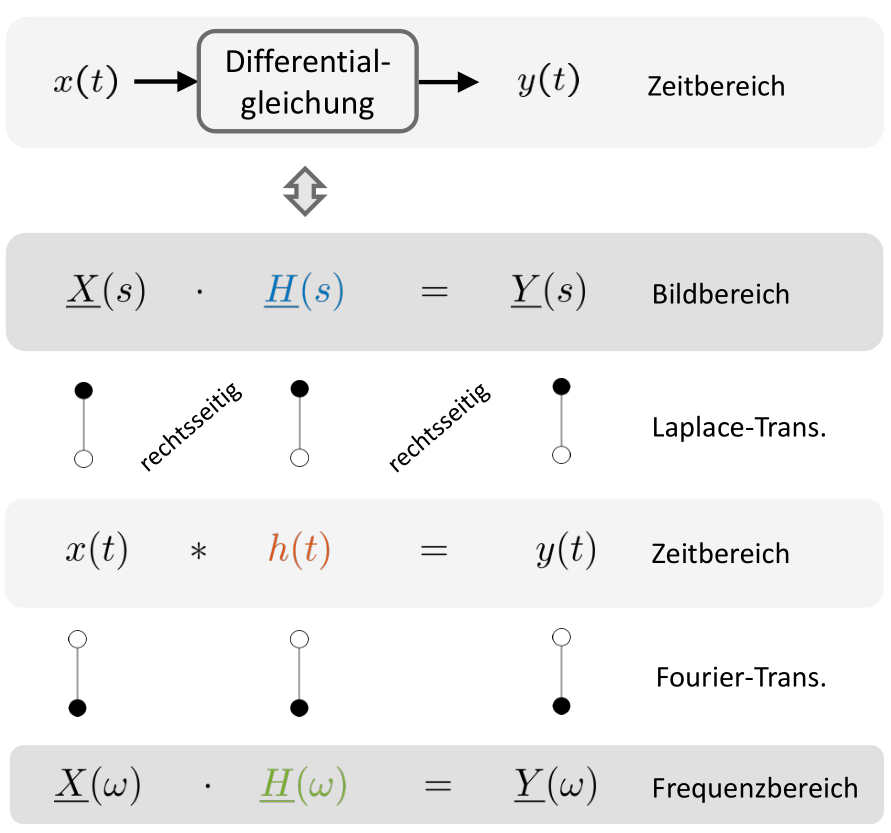
\includegraphics[width=0.98\columnwidth]{Bilder/LTI_Systemantworten.png}
%\clearpage
\subsection{Eigenschaften der LPT}
\renewcommand{\arraystretch}{1.7}
\begin{tabularx}{\columnwidth}{|X|X|X|}
	\hline
	& $\mathbf{x(t)}$ & \underline{$\mathbf{X}$}$\mathbf{(s)}$\\
	\hline Linearität & $a x_{1}(t)+b x_{2}(t)$ & $a \underline{X}_{1}(s)+b\underline{X}_{2}(s)$ \\
	\hline Skalierung $t$ & $x(at)$ & $\frac{1}{a} \underline{X}(\frac{s}{a})$ \\
	\hline Skalierung $s$ & $\frac{1}{a} \, x(\frac{t}{a})$ & $\underline{X}(as)$ \\
	\hline Verschiebung	& $x(t-t_0)$ & $e^{-s \cdot t_0} \underline{X}(s)$ \\
	\hline Modulation & $e^{at} \, x(t)$ & $\underline{X} (s-a)$ \\
	\hline Multiplikation & $t \cdot x(t) $ & $-\frac{d}{d s} \underline{X}(s)$ \\
	\hline Faltung & $x_{1}(t) * x_{2}(t) $ & $ \underline{X}_{1}(s) \cdot \underline{X}_{2}(s)$ \\
	\hline Differentiation $t$ & $ \frac{d}{dt} x(t) $ & $ s\cdot \underline{X}(s)-x(0^-)$ \\
	\hline Integration $t$ & $\int_{0}^{t} x(\tau) \, d\tau $ & $ \frac{1}{s} \underline{X}(s)$ \\
	\hline Integration $s$ & $\frac{1}{t} \cdot x(t) $ & $ \int_{s}^{\infty} \underline{X}(s) \, ds$ \\
	\hline
\end{tabularx}

\subsubsection{Grenzwertsätze}
\begin{itemize}
	\item Anfangswertsatz 
	$$x(0+) = \lim_{s\to\infty} s\cdot \underline{X}(s)$$
	\item Endwertsatz 
	$$x(\infty) = \lim_{s\to 0} s\cdot \underline{X}(s)$$
\end{itemize}

\clearpage
\end{multicols*}
\begin{table}[h!]
	\subsection{Korrespondenzen der LPT}\label{lpt_tabelle}
	\renewcommand{\arraystretch}{1.7}
\begin{minipage}[t]{0.5\columnwidth}
	\begin{tabularx}{\columnwidth}{|l|l|X|}
		\hline
		Nr. & $\mathbf{x(t)}$ für $t \geq 0$ & $\mathbf{\underline{X}(s)}$ \\
		\hline 
		10 & 1 & $\frac{1}{s}$ \\
		\hline
		11 & $t$ & $\frac{1}{s^2}$ \\
		\hline
		12 & $\frac{t^n}{n!}$ & $\frac{1}{s^{n+1}}$ \\
		\hline
		13 & $\mathrm{e}^{-a t}$ & $\frac{1}{s+a}$ \\
		\hline
		14 & $\frac{1}{a} \cdot\left(1-\mathrm{e}^{-a t}\right)$ & $\frac{1}{s(s+a)}$ \\
		\hline
		15 & $\sin (a t)$ & $\frac{a}{s^2+a^2}$ \\
		\hline
		16 & $\sinh (a t)$ & $\frac{a}{s^2-a^2}$ \\
		\hline
		17 & $\cos (a t)$ & $\frac{s}{s^2+a^2}$\\
		\hline
		18 & $\cosh (a t)$ & $\frac{s}{s^2-a^2}$\\
		\hline
		19 & $t \cdot \mathrm{e}^{-a t}$ & $\frac{1}{(s+a)^2}$\\
		\hline
		20 & $(1-a t) \cdot \mathrm{e}^{-a t}$ & $\frac{s}{(s+a)^2}$\\
		\hline 21 & $\frac{1}{a^2} \cdot\left[1-(1+a t) \cdot \mathrm{e}^{-a t}\right]$ &
		$\frac{1}{s(s+a)^2}$ \\
		\hline 22 & 
		$\frac{t^2}{2} \cdot \mathrm{e}^{-a t}$ & 	$\frac{1}{(s+a)^3}$	\\
		\hline 23 & 	$\frac{1}{a^2} \cdot(1-\cos a t)$ & 	$\frac{1}{s\left(s^2+a^2\right)}$ \\
		\hline 24 & 	$\frac{1}{a^2} \cdot(\cosh a t-1)$ & 	$\frac{1}{s\left(s^2-a^2\right)}$\\
		\hline 25 & 	$\frac{1}{a^2} \cdot\left[a t-1+\mathrm{e}^{-a t}\right]$ & $\frac{1}{s^2(s+a)}$ \\
		\hline 26 & 	$\frac{\mathrm{e}^{-a t}-\mathrm{e}^{-b t}}{b-a}$& 	$\frac{1}{(s+a) \cdot(s+b)}$\\
		\hline 27 & 	$\frac{a \cdot \mathrm{e}^{-a t}-b \cdot \mathrm{e}^{-b t}}{a-b}$ & 	$\frac{s}{(s+a) \cdot(s+b)}$ \\
		\hline
	\end{tabularx}
\end{minipage}
\begin{minipage}{0.5\columnwidth}
\begin{tabularx}{\columnwidth}{|l|l|X|}
			\hline
	Nr. & $\mathbf{x(t)}$ für $t \geq 0$ & $\mathbf{\underline{X}(s)}$ \\
			\hline 28 & 
	$\frac{1}{a b}+\frac{b \cdot \mathrm{e}^{-a t}-a \cdot \mathrm{e}^{-b t}}{a b \cdot(a-b)}$
	& 
	$\frac{1}{s(s+a)(s+b)}$
	\\	
		\hline 29 & 
		$\frac{\mathrm{e}^{-a t}+[(a-b) t-1] \cdot \mathrm{e}^{-b t}}{(a-b)^2}$
		& 
		$\frac{1}{(s+a)(s+b)^2}$
		\\
		\hline 30 & 
		$\frac{[a-b(a-b) t] \cdot \mathrm{e}^{-b t}-a \cdot \mathrm{e}^{-a t}}{(a-b)^2}$
		& 
		$\frac{s}{(s+a)(s+b)^2}$
		\\
		\hline 31 & 
		$\frac{(b-c) \cdot \mathrm{e}^{-a t}+(c-a) \cdot \mathrm{e}^{-b t}+(a-b) \cdot \mathrm{e}^{-c t}}{(b-a)(c-a)(b-c)}$ & 
		$\frac{1}{(s+a)(s+b)(s+c)}$ \\
		\hline 32 & 
		$\frac{a(b-c) \cdot \mathrm{e}^{-a t}+b(c-a) \cdot \mathrm{e}^{-b t}+c(a-b) \cdot \mathrm{e}^{-c t}}{(b-a)(c-b)(c-a)}$ & $\frac{s}{(s+a)(s+b)(s+c)}$ \\
		\hline 33 & $\frac{1}{2 \omega^3} \cdot(\sin \omega t-\omega t \cdot \cos \omega t)$ & $\frac{1}{\left(s^2+\omega^2\right)^2}$ \\
		\hline 34 & $\frac{t}{2 \omega} \cdot \sin \omega t$ & $\frac{s}{\left(s^2+\omega^2\right)^2}$ \\
		\hline 35 & $\frac{1}{2 \omega} \cdot(\sin \omega t+\omega t \cdot \cos \omega t)$ & $\frac{s^2}{\left(s^2+\omega^2\right)^2}$ \\
		\hline 36 & $\sin ^2(\omega t)$ & 
		$\frac{2 \omega^2}{s\left(s^2+4 \omega^2\right)}$ \\
		\hline 37 & $\cos ^2(\omega t)$ & 
		$\frac{s^2+2 \omega^2}{s\left(s^2+4 \omega^2\right)}$ \\
		\hline 38 & $\cos (\omega t+\psi)$ & 
		$\frac{s \cos \psi-\omega \sin \psi}{s^2+\omega^2}$ \\
		\hline 39 & $\sin (\omega t+\psi)$ & $\frac{s \sin \psi+\omega \cos \psi}{s^2+\omega^2}$ \\
		\hline 40 & $\mathrm{e}^{-a t} \cdot \cos (\omega t)$ & 
		$\frac{s+a}{(s+a)^2+\omega^2}$ \\
		\hline 41 & $\mathrm{e}^{-a t} \cdot \sin (\omega t)$ & 
		$\frac{\omega}{(s+a)^2+\omega^2}$ \\
		\hline 42 & $\mathrm{e}^{-a t} \cdot \cos (\omega t+\psi)$ & 
		$\frac{(s+a) \cos \psi-\omega \sin \psi}{(s+a)^2+\omega^2}$ \\
		\hline 43 & 
		$\frac{a \cos \omega t+\omega \sin \omega t-a \cdot \mathrm{e}^{-a t}}{a^2+\omega^2}$ &
		$\frac{s}{s^2+\omega^2} \cdot \frac{1}{s+a}$\\
		\hline 44 & 
		$\frac{a \sin \omega t-\omega \cos \omega t+\omega \cdot \mathrm{e}^{-a t}}{a^2+\omega^2}$ & 
		$\frac{\omega}{s^2+\omega^2} \cdot \frac{1}{s+a}$ \\
		\hline 45 & 
		$\frac{\cos (\omega t+\psi-\gamma)-\cos (\psi-\gamma) \cdot \mathrm{e}^{-a t}}{\sqrt{a^2+\omega^2}}$ & 
		$\frac{s \cos \psi-\omega \sin \psi}{\left(s^2+\omega^2\right) \cdot(s+a)}$ \\
		\hline
	\end{tabularx}
\end{minipage}
\end{table}
\noindent
\begin{minipage}{0.7\columnwidth}
	\renewcommand{\arraystretch}{1.5}
	\begin{tabular}{|l|c|c|}
		\hline Nr  & $\mathbf{x(t)}$ für $t \geq 0$ & $\mathbf{\underline{X}(s)}$ \\
		\hline 46  & \begin{tabular}{l}
			\begin{tabular}{l}
				$a^2>b^2: \quad \frac{1}{2 W} \cdot\left(\mathrm{e}^{\lambda_1 t}-\mathrm{e}^{\lambda_2 t}\right)$ \\
				$a^2=b^2: \quad t \cdot \mathrm{e}^{-a t}$ \\
				$a^2<b^2: \quad \frac{1}{\omega_d} \cdot \mathrm{e}^{-a t} \cdot \sin \omega_{\mathrm{d}} t$
			\end{tabular}
		\end{tabular} & $\dfrac{1}{s^2+2 a s+b^2}$\\
		\hline 47   & \begin{tabular}{l}
			\begin{tabular}{l}
				$a^2>b^2: \quad \frac{1}{2 W} \cdot\left(\lambda_1 \mathrm{e}^{\lambda_1 t}-\lambda_2 \mathrm{e}^{\lambda_2 t}\right)$ \\
				$a^2=b^2: \quad (1-a t) \cdot \mathrm{e}^{-a t}$ \\
				$a^2<b^2: \quad \left(\cos \omega_{\mathrm{d}} t-\frac{a}{\omega_{\mathrm{d}}} \cdot \sin \omega_{\mathrm{d}} t\right) \cdot \mathrm{e}^{-a t}$
			\end{tabular}
		\end{tabular} & 
			$\dfrac{s}{s^2+2 a s+b^2}$ \\
		\hline 48 & \begin{tabular}{l}
			\begin{tabular}{l}
				$a^2>b^2: \quad \frac{1}{b^2}\left(1+\frac{\lambda_2}{2 W} \cdot \mathrm{e}^{\lambda_1 t}-\frac{\lambda_1}{2 W} \cdot \mathrm{e}^{\lambda_2 t}\right)$ \\
				$a^2=b^2: \quad \frac{1}{a^2}\left[1-(1+a t) \cdot \mathrm{e}^{-a t}\right]$ \\
				$a^2<b^2: \quad \frac{1}{b^2}\left[1-\left(\cos \omega_{\mathrm{d}} t+\frac{a}{\omega_{\mathrm{d}}} \cdot \sin \omega_{\mathrm{d}} t\right) \cdot \mathrm{e}^{-a t}\right]$
			\end{tabular}
		\end{tabular} & 
			$\dfrac{1}{s\left(s^2+2 a s+b^2\right)}$
		 \\
		\hline 49 &
			\begin{tabular}{l}
				$a^2>b^2: \quad \frac{\cos (\omega_0 t+\varphi)+k_1 \cdot \mathrm{e}^{-\lambda_1 t}+k_2 \cdot \mathrm{e}^{-\lambda_2 t}}{\sqrt{x^2+y^2}}$ \\
				$a^2=b^2: \quad \frac{\cos (\omega_0 t+\varphi)+(z t-\cos \varphi) \cdot \mathrm{e}^{-a t}}{\sqrt{x^2+y^2}}$ \\
				$a^2<b^2: \quad \frac{\cos (\omega_0 t+\varphi)-k \cdot \cos \left(\omega_{\mathrm{d}} t+\beta\right) \cdot \mathrm{e}^{-a t}}{\sqrt{x^2+y^2}}$
			\end{tabular}
		 & 
			$\frac{s \cos \psi-\omega \sin \psi}{\left(s^2+\omega^2\right) \cdot\left(s^2+2 a s+b^2\right)}$
		\\
		\hline
	\end{tabular}
\end{minipage}
\begin{minipage}{0.25\columnwidth}
%{\centering
%\small
\begin{itemize}[leftmargin=*]
	\item Aperiodischer Kriechfall:\\
	$a^2>b^2 \quad \leftrightarrow \quad \vartheta>1$
	
	\item Aperiodischer \textbf{Grenzfall:}\\
	$a^2=b^2 \quad \leftrightarrow \quad \vartheta=1$
	
	\item Periodischer Schwingfall:\\
	$a^2<b^2 \quad \leftrightarrow \quad 0<\vartheta<1$
	
	\item Abklingkonstante:\\
	$a=\delta =\dfrac{\vartheta}{T} = \vartheta\,\omega_0 = \dfrac{R}{2L}$
	
	\item Resonanz-Kreisfrequenz:\\
	$b=\omega_0=\dfrac{1}{T} =\dfrac{1}{\sqrt{LC}}$
	
	\item Eigen-Kreisfrequenz:\\
	$\omega_d = \sqrt{b^2-a^2} \\
	= \sqrt{\omega_0^2-\delta^2} = \omega_0\sqrt{1-\vartheta^2}$
	
	\item Dämpfungsgrad,-maß, -konstante:\\
	$\vartheta = D =  \dfrac{\delta}{\omega_0} = \dfrac{a}{b}$
\end{itemize} 
%}
\end{minipage}\\
$\arraycolsep=1.7pt\def\arraystretch{1.7}
\begin{array}{cccc}
	\lambda_{1,2}=-a\pm W = -a\pm j\omega_d & \quad W=\sqrt{a^2-b^2}=j\omega_d & \quad x=b^2-\omega^2$ \qquad $y=2a\omega & \quad z=\omega \sin\varphi - a \cos \varphi\\
	\varphi=\arctan\dfrac{x\sin\varphi-y\cos\varphi}{y\sin\varphi+x\cos\varphi} & k=\dfrac{\cos\varphi}{\cos\beta} & k_1=\dfrac{\lambda_2\cos\varphi-\omega\sin\varphi}{2W} & k_2=\dfrac{\omega\sin\varphi-\lambda_1\cos\varphi}{2W}
\end{array}$\\
\vspace{1.5em}
$\beta=\arctan\dfrac{z}{\omega_d \, \cos\varphi}$
\newpage
\begin{multicols*}{2}
%\begin{mdframed}[style=exercise,nobreak=false]
%	\begin{itemize}
%		\item \textbf{Linearität}
%		      \[
%			      \alpha x_1(t) + \beta x_2(t) \ \laplace\  \alpha \underline{X}_1(t) + \beta \underline{X}_2(t)
%		      \]
%		      \vspace{-1.5em}
%		\item \textbf{Skalierung im Zeitbereich}
%		      \[
%			      x(\alpha t) \ \laplace\  \frac{1}{\alpha} \underline{X}\left(\frac{s}{\alpha}\right) \qquad \color{red}{\alpha > 0}
%		      \]
%		      \vspace{-1.5em}
%		\item \textbf{Skalierung im Bildbereich}
%		      \[
%			      \frac{1}{\alpha}x\left(\frac{t}{\alpha}\right)\ \laplace\ \underline{X}(\alpha s) \qquad \color{red}{\alpha > 0}
%		      \]
%		      \vspace{-1.5em}
%		\item \textbf{Verschiebung im Zeitbereich}
%		      \[
%			      x(t-t_0)\ \laplace\ e^{-st_0} \underline{X}(s) \qquad \color{red}{t_0 > 0}
%		      \]
%		      \vspace{-1.5em}
%		\item \textbf{Verschiebung im Bildbereich - Modulation}
%		      \[
%			      e^{at}x(t) \ \laplace\ \underline{X}(s-a)
%		      \]
%		      \vspace{-1.5em}
%		\item \textbf{Faltung}
%		      \[
%			      x_1(t)*x_2(t) \ \laplace\ \underline{X}_1(s)\cdot \underline{X}_2(s)
%		      \]
%		      \vspace{-1.5em}
%		\item \textbf{Differentiation im Zeitbereich}
%		      \[
%			      \frac{d}{dt}x(t) \ \laplace\ s\cdot\underline{X}(s)\color{red}{-x(0^+)}
%		      \]
%		      \vspace{-1.5em}
%		\item \textbf{Differentiation im Bildbereich}
%		      \[
%			      t\cdot x(t) \ \laplace\ -\frac{d}{ds}\underline{X}(s)
%		      \]
%		      \vspace{-1.5em}
%		\item \textbf{Integration im Zeitbereich}
%		      \[
%			      \int_0^t x(\tau)d\tau \ \laplace\ \frac{1}{s}\underline{X}(s)
%		      \]
%		      \vspace{-1.5em}
%		\item \textbf{Integration im Bildbereich}
%		      \[
%			      \frac{1}{t}x(t) \ \laplace\ \int_s^\infty\underline{X}(s)ds
%		      \]
%	\end{itemize}
%\end{mdframed}
%\subsubsection{Rücktransformation rationaler Funktionen}
%\footnotesize
%Partialbruchzerlegung: Siehe papula nach S.157

\section{Schaltvorgänge}
\subsection{Berechnungsmethoden}
Immer \textbf{Stetigkeitsbedingungen} beachten!
\[
\boxed{x(t=0) = x(0) = x(0^-) = x(0^+)}
 \]
Bauteilverhalten KS/LL:
 $\underline{X}_C=-j\frac{1}{\omega C}$ \quad $\underline{X}_L =j \omega L$
\subsubsection{Vereinfachte Methode}
mit Lösungsformeln aus GE1, GE2.
\begin{itemize}
	\item \textbf{Bedingung}: \textbf{konstantes} Eingangssignal/Quelle und \textbf{einem} unabhängigem Energiespeicher $L$ \textbf{oder} $C$ (DGL 1. Ordnung, \textbf{eine} Zeitkonstante).
	\item GE1: Schaltung mit \textbf{einer} Induktivität $L$:
	\begin{gather*}
		\tau=\frac{L}{R} \qquad I_A = i(0) \qquad I_E=i(t\rightarrow\infty)\\
		\boxed{i(t)=I_E+(I_A-I_E)\cdot e^{-t/\tau}}
	\end{gather*}
	\item GE2: Schaltung mit \textbf{einer} Kapazität $C$:
	\begin{gather*}
		\tau=RC \qquad U_A = u(0) \qquad U_E=u(t\rightarrow\infty)\\
		\boxed{u(t)=U_E+(U_A-U_E)\cdot e^{-t/\tau}}
	\end{gather*}
	
\end{itemize}

\subsubsection{Laplace-Transformation der DGL}
\begin{enumerate}
	\item DGL aufstellen mit Bauteilgleichungen f\"ur $R,L,C$. Maschen- und Knotensatz anwenden.
	\item LPT der DGL durchführen:
	\[
	 \dot{x}(t) \ \laplace\ s\cdot\underline{X}(s)-x(0^+)
	\]
	\[
	\ddot{x}(t) \ \laplace\ s^2\cdot\underline{X}(s)-s\cdot x(0^+)-\frac{dx}{dt}(0^+)
	\]
	Anfangszustand $i_L, u_C \neq 0$ zum Schaltzeitpunkt $x(0^+)$ wird autom. \textbf{berücksichtigt}.
	\item Auflösen nach gesuchter Größe.
	\item Rücktransformation in Zeitbereich mit \textbf{Tabelle}.
\end{enumerate}

\subsubsection{Leere Energiespeicher mit LPT \& KWR}
\begin{enumerate}
	\item \textbf{Bedingung}: Alle $C$ ungeladen, Alle $L$ stromlos.
	\[ 
	 u_c(0+) = i_L(0+) = 0
	 \]

	\item Eingang $x(t)$ mit LPT in Bildbereich $\underline{X}(\omega)$.
    \item $\underline{H}(s)$ aus Schaltung \underline{nach}
        Schaltvorgang mit erweiteter KWR bestimmen. Ersetze $s = j\omega $.
    \item Ausgang im Bildbereich berechnen: $\underline{Y}(s) =
        \underline{X}(s)\cdot \underline{H}(s)$
    \item Rücktransformation in Zeitbereich mit \textbf{Tabelle}.
    
\end{enumerate}
\subsubsection{Geladene Energiespeicher mit LPT}
\begin{enumerate}
    \item Ersatzschaltbild (ESB) für Schaltkreis nach dem
        Schaltvorgang im Bildbereich erstellen:
        \begin{itemize}
        	\item VZ beachten! VZ-Änderung im Zeitbereich auch im Bildbereich gültig!
            \item Induktivitäten mit Anfangsstrom:
            
                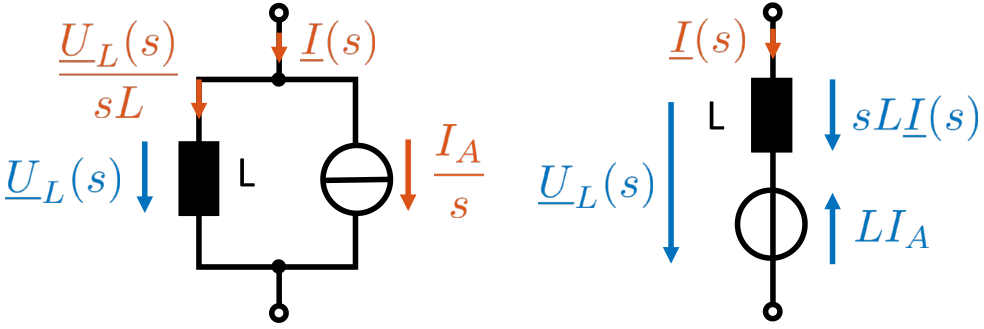
\includegraphics[width=0.4\textwidth]{Bilder/ESB_Fuer_stromfuehrende_Induktivitaet}
                
                \begin{align*}
                    \underline{U}_L(s) &= L\cdot(s\cdot\underline{I}_L(s)-\underbrace{i_L(0)}_{I_A})\\
                    \underline{I}_L(s) &= \frac{\underline{U}_L(s)}{sL}+\frac{I_A}{s}
                \end{align*}
            \item Kapazitäten mit Anfangsspannung/Vorladung:
                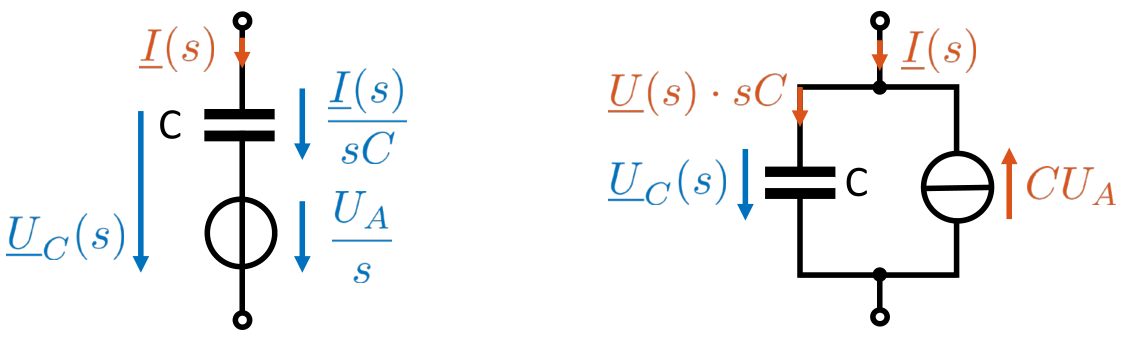
\includegraphics[width=0.4\textwidth]{Bilder/ESB_Fuer_geladene_Kapazitaet}
                \begin{align*}
                    \underline{I}_C(s) &= C\cdot(s\cdot\underline{U}_C(s)-\underbrace{u_C(0)}_{U_A})\\
                    \underline{U}_C(s) &= \frac{\underline{I}_C(s)}{sC}+\frac{U_A}{s}
                \end{align*}
        \end{itemize}
    \item $\underline{H}(s)$ aus ESB mit KWR bestimmen.
    \item Eingang $x(t)$ mit LPT in Bildbereich $\underline{X}(\omega)$.
    \item Ausgang im Bildbereich berechnen: $\underline{Y}(s) =
        \underline{X}(s)\cdot \underline{H}(s)$
    \item Rücktransformation in Zeitbereich mit \textbf{Tabelle}.
\end{enumerate}
\subsection{Quellenumwandlung}
\begin{gather*}
	\text{Stromquelle: }i_q(t)\cdot \varepsilon(t) \quad \laplace \quad \frac{I_q(s)}{s}\\
	\text{Spannungsquelle: }u_q(t)\cdot \varepsilon(t) \quad \laplace \quad \frac{U_q(s)}{s}
\end{gather*}
\subsection{Bauteilgleichungen}
\begin{gather*}
	i_L (t) = C \cdot \frac{du_c(t)}{dt} \qquad u_L (t) = L \cdot \frac{di_c(t)}{dt}
\end{gather*}
\newpage
%\end{multicols*}
\section{Zeitdiskrete Systeme}
\subsection{Elementare, zeitdiskrete Signale}
	\begin{itemize}[leftmargin=*]
		\item \textbf{Einheitsimpuls}, Impulsfolge, Delta-Impuls $\delta(n)$\\
		      \makebox[\columnwidth][c]
		      {
			      \begin{minipage}{0.3\columnwidth}
				      \[ \boxed{
					      \delta(n) =
					      \begin{cases}
						      1 & n = 0    \\
						      0 & n \neq 0
					      \end{cases}
					    }
				      \]
			      \end{minipage}
			      \begin{minipage}{0.7\columnwidth}
				      \centering
				      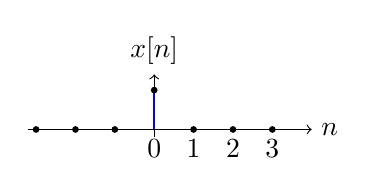
\begin{tikzpicture}[baseline=0.8,scale=0.5]
					      \draw[->] (0,-0.2) -- (0,1.4) node[above]{$x[n]$}; %y
					      \draw[->] (-3.2,0) -- (4,0) node[right]{$n$}; %x
					      \filldraw[black] (-3,0) circle (2pt) {};
					      \filldraw[black] (-2,0) circle (2pt) {};
					      \filldraw[black] (-1,0) circle (2pt) {};
					      \draw[blue, thick] (0,1) -- (0,0) node[below, black]{0}; \filldraw[black] (0,1) circle (2pt) {};
					      \filldraw[black] (1,0) circle (2pt) node[below]{1};
					      \filldraw[black] (2,0) circle (2pt) node[below]{2};
					      \filldraw[black] (3,0) circle (2pt) node[below]{3};
				      \end{tikzpicture}
			      \end{minipage}
		      }\\
		      
		      Eigenschaften:
		      \begin{itemize}
		      	  \item Zusammenhang mit Einheitssprung:
		      	  $$\sum^{\infty}_{n=-\infty}\delta(n)=1 \qquad \boxed{ \varepsilon(n)=\sum_{k=-\infty}^{n} \delta(n) } $$
			      \item Anregung der Impulsantwort
			      \item konstantes Spektrum
			      \item Ausblendeigenschaft:
			      \[
			      x(n) = \sum_{k=-\infty}^{\infty} x(k)\cdot\delta(n-k)
			      \]
		      \end{itemize}

		\item \textbf{Einheitssprung}\\
		      \makebox[\columnwidth][c]
		      {
			      \begin{minipage}{0.3\columnwidth}
				      \[
					      \varepsilon(n) =
					      \begin{cases}
						      1 & n \geq 0 \\
						      0 & n < 0
					      \end{cases}
				      \]
			      \end{minipage}
			      \begin{minipage}{0.7\columnwidth}
				      \centering
				      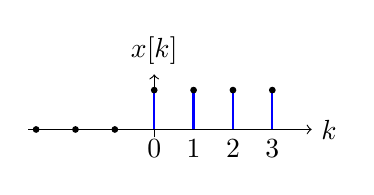
\begin{tikzpicture}[baseline=0.8,scale=0.5]
					      \draw[->] (0,-0.2) -- (0,1.4) node[above]{$x[k]$}; %y
					      \draw[->] (-3.2,0) -- (4,0) node[right]{$k$}; %x
					      \filldraw[black] (-3,0) circle (2pt) {};
					      \filldraw[black] (-2,0) circle (2pt) {};
					      \filldraw[black] (-1,0) circle (2pt) {};
					      \draw[blue, thick] (0,1) -- (0,0) node[below, black]{0}; \filldraw[black] (0,1) circle (2pt) {};
					      \draw[blue, thick] (1,1) -- (1,0) node[below, black]{1}; \filldraw[black] (1,1) circle (2pt) {};
					      \draw[blue, thick] (2,1) -- (2,0) node[below, black]{2}; \filldraw[black] (2,1) circle (2pt) {};
					      \draw[blue, thick] (3,1) -- (3,0) node[below, black]{3}; \filldraw[black] (3,1) circle (2pt) {};
				      \end{tikzpicture}
			      \end{minipage}
		      }
		      Zusammenhang mit Einheitsimpuls:
		      \[ \boxed{
			      \delta(n) = \varepsilon(n) - \varepsilon(n-1) }
		      \]
		\item \textbf{Rechteckfolge}\\
		      \makebox[\columnwidth][c]
		      {
			      \begin{minipage}{0.3\columnwidth}
				      \[
					      \operatorname{rect}_N(n) =
					      \begin{cases}
						      1 & 0 \leq n < N   \\
						      0 & \texttt{sonst}
					      \end{cases}
				      \]
			      \end{minipage}
			      \begin{minipage}{0.7\columnwidth}
				      \centering
				      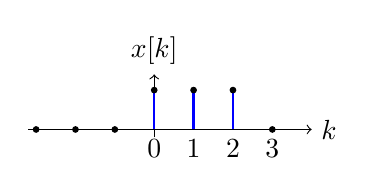
\begin{tikzpicture}[baseline=0.8,scale=0.5]
					      \draw[->] (0,-0.2) -- (0,1.4) node[above]{$x[k]$}; %y
					      \draw[->] (-3.2,0) -- (4,0) node[right]{$k$}; %x
					      \filldraw[black] (-3,0) circle (2pt) {};
					      \filldraw[black] (-2,0) circle (2pt) {};
					      \filldraw[black] (-1,0) circle (2pt) {};
					      \draw[blue, thick] (0,1) -- (0,0) node[below, black]{0}; \filldraw[black] (0,1) circle (2pt) {};
					      \draw[blue, thick] (1,1) -- (1,0) node[below, black]{1}; \filldraw[black] (1,1) circle (2pt) {};
					      \draw[blue, thick] (2,1) -- (2,0) node[below, black]{2}; \filldraw[black] (2,1) circle (2pt) {};
					      \filldraw[black] (3,0) circle (2pt) node[below] {3};
				      \end{tikzpicture}
			      \end{minipage}
		      }
		      Zusammenhang mit Einheitsimpuls bzw. -sprung:
		      \begin{align*}
			      \operatorname{rect}(n) & = \varepsilon(n) + \varepsilon(n-N)       \\
			                             & = \varepsilon(n) \cdot \varepsilon(N-1-n)
			                             \\
			                             & = \sum_{k=0}^{N-1} \delta(n-k)
		      \end{align*}
		\item \textbf{Zeitdiskreter Sinus}\\
		      \makebox[\columnwidth][c]
		      {
			      \begin{minipage}{0.3\columnwidth}
				      \[
					      x(n) = A \cdot \sin(\Omega\, n+\varphi)
				      \]
				      \small
				      
				      $A$       : Amplitude            \\
				      $\Omega$  : normierte\\ Kreisfrequenz \\
				      $\varphi$ : Anfangsphase
				      
				      \normalsize
				      
%  		      \begin{align*}
%				      	A       & :\texttt{Amplitude}               \\
%				      	\Omega  & :\texttt{normierte Kreisfrequenz} \\
%				      	\varphi & :\texttt{Anfangsphase}
%				\end{align*}
			      \end{minipage}
			      \begin{minipage}{0.7\columnwidth}
				      \centering
				      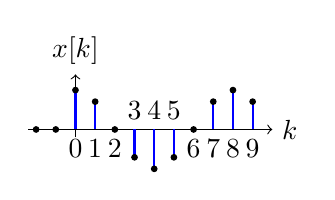
\begin{tikzpicture}[baseline=1,scale=0.5]
					      \draw[->] (0,-0.2) -- (0,1.4) node[above]{$x[k]$}; %y
					      \draw[->] (-1.2,0) -- (5,0) node[right]{$k$}; %x
					      \filldraw[black] (-1,0) circle (2pt) {};
					      \filldraw[black] (-0.5,0) circle (2pt) {};
					      \draw[blue,thick] (0,1) -- (0,0)          node[below, black]{0}; \filldraw[black] (0,1) circle (2pt) {};
					      \draw[blue,thick] (0.5,0.707) -- (0.5,0)  node[below, black]{1}; \filldraw[black] (0.5,0.707) circle (2pt) {};
					      \filldraw[black] (1,0) circle (2pt)              node[below, black]{2};
					      \draw[blue,thick] (1.5,-0.707) -- (1.5,0) node[above, black]{3}; \filldraw[black] (1.5,-0.707) circle (2pt) {};
					      \draw[blue,thick] (2,-1) -- (2,0)         node[above, black]{4}; \filldraw[black] (2,-1) circle (2pt) {};
					      \draw[blue,thick] (2.5,-0.707) -- (2.5,0) node[above, black]{5}; \filldraw[black] (2.5,-0.707) circle (2pt) {};
					      \filldraw[black] (3,0) circle (2pt)              node[below]{6};
					      \draw[blue,thick] (3.5,0.707) -- (3.5,0)  node[below, black]{7}; \filldraw[black] (3.5,0.707) circle (2pt) {};
					      \draw[blue,thick] (4,1) -- (4,0)          node[below, black]{8}; \filldraw[black] (4,1) circle (2pt) {};
					      \draw[blue,thick] (4.5,0.707) -- (4.5,0)  node[below, black]{9}; \filldraw[black] (4.5,0.707) circle (2pt) {};
				      \end{tikzpicture}
			      \end{minipage}
		      }

		\item \textbf{Komplexe Exponentialfolge}\\
		      \makebox[\columnwidth][c]
		      {
			      \begin{minipage}{0.3\columnwidth}
				      \begin{align*}
					      x(n) & = \underline{A} \cdot e^{Sn}                \\
					           & = \underline{A} \cdot e^{(\Sigma+j\Omega)n}
				      \end{align*}
			      \end{minipage}
			      \begin{minipage}{0.7\columnwidth}
				      \centering
				      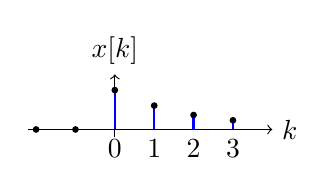
\begin{tikzpicture}[baseline=0.8,scale=0.5]
					      \draw[->] (0,-0.2) -- (0,1.4) node[above]{$x[k]$}; %y
					      \draw[->] (-2.2,0) -- (4,0) node[right]{$k$}; %x
					      \filldraw[black] (-2,0) circle (2pt) {};
					      \filldraw[black] (-1,0) circle (2pt) {};
					      \draw[blue, thick] (0,1) -- (0,0) node[below, black]{0}; \filldraw[black] (0,1) circle (2pt) {};
					      \draw[blue, thick] (1,0.606) -- (1,0) node[below, black]{1}; \filldraw[black] (1,0.606) circle (2pt) {};
					      \draw[blue, thick] (2,0.367) -- (2,0) node[below, black]{2}; \filldraw[black] (2,0.367) circle (2pt) {};
					      \draw[blue, thick] (3,0.233) -- (3,0) node[below, black]{3}; \filldraw[black] (3,0.233) circle (2pt) {};
				      \end{tikzpicture}
			      \end{minipage}
		      }
		      \begin{align*}
			      S                                       & = \Sigma+j\Omega        \\
			      \texttt{Amplitudenänderung }\Sigma      & = \sigma T = \sigma/f_A \\
			      \texttt{normierte Kreisfrequenz }\Omega & = \omega T =  2\pi \frac{f_0}{f_A}
		      \end{align*}
	\end{itemize}
%	\clearpage
%\begin{multicols*}{2}
\subsection{A/D-Wandlung}
\small
\begin{itemize}
	\item Zeitdiskretisierung, Abtastung, \textbf{Abtastrate}: $\boxed{f_a = \dfrac{1}{t_a}}$
	\[
	x(n)= x_0(t)\big|_{t = n{T_a}} = x_0 (nT) = x_0\left(\frac{n}{f_a}\right)
	\]
	\item Wertdiskretisierung (Quantisierung): Bitbreite, Aufl\"osung: 8 Bit = 256 Stufen.
	\item Abtastung Analog-Signal $\rightarrow$ \textbf{periodische} Fortsetzung des Analog-Spektrums im Abstand von $$ \boxed{
	\omega_a=\frac{2\pi}{t_a}=2\pi f_a \text{\qquad mit } t_a\text{: Abtastintervall} }$$
	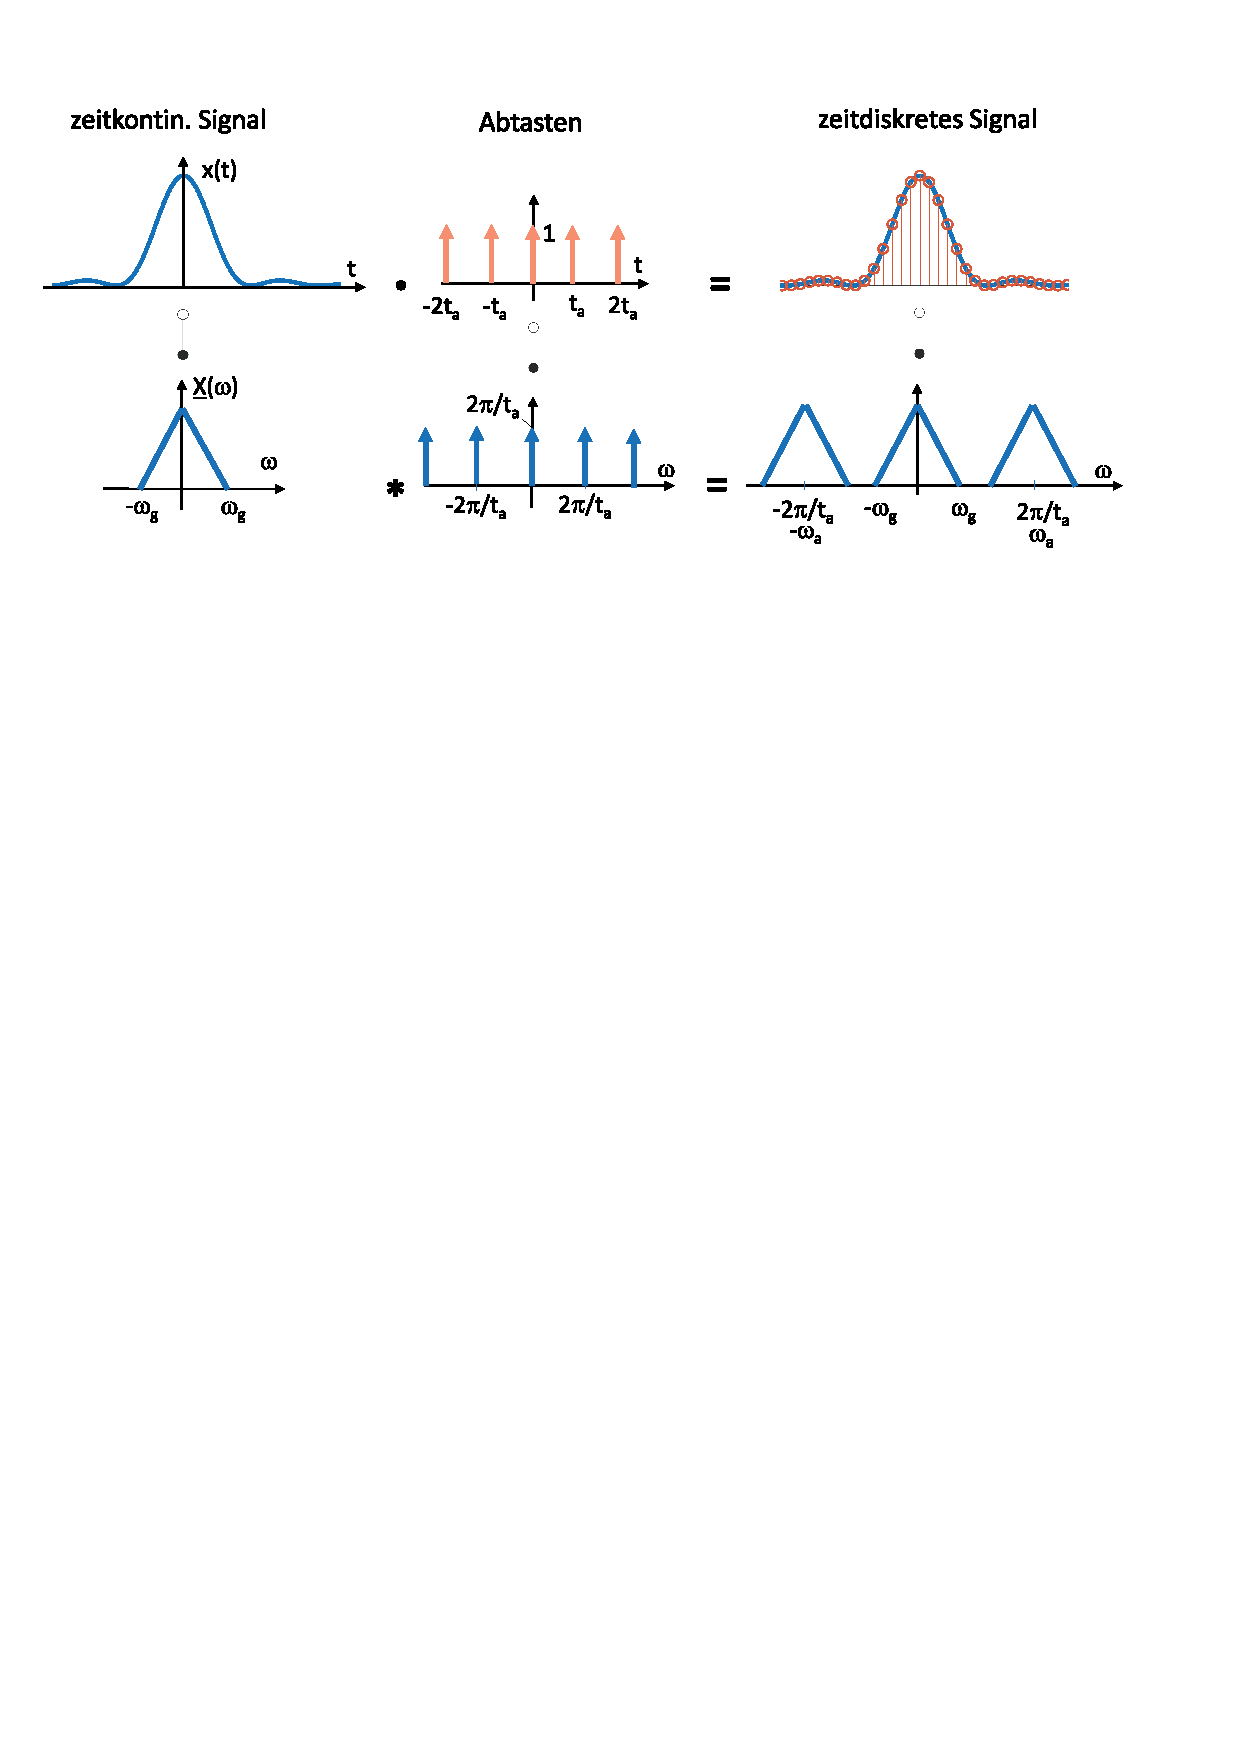
\includegraphics[width=0.9\columnwidth]{Bilder/Abtastung_Frequenzbereich_Spektrum_Original}
	\item \textbf{Aliasing}: {\small Spektrale \"Uberlagerung, zus\"atzliche Frequenzen/Abtastwerte, keine Rekonstruktion des Originalsignals aus $t_a=\frac{1}{f_a}$ m\"oglich.\\
				
	\textit{Abhilfe}: Eingangssignal auf $\omega_g$-Band begrenzen und\\ \textbf{Abtasttheorem} einhalten, Verringerung von $t_a$.}
\normalsize
\begin{gather*}
	\boxed{\omega_a \ge 2 \omega_g} \text{ bzw. } f_a \ge 2 f_g\\
	\boxed{\omega_g \le \frac{\omega_a}{2}} = \frac{1}{2} \cdot \frac{2\pi}{t_a} \text{ bzw. } f_g \ge \frac{f_a}{2}
\end{gather*}
%\begin{figure}[h!]
%	\centering
%	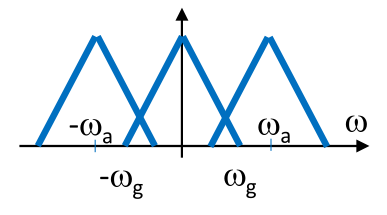
\includegraphics[width=\columnwidth]{Bilder/Abtasttheorem_Uebrlappung}
%\end{figure}
{\footnotesize Merke: zeitbegrenztes Signal: $\infty$ langes Spektrum $\rightarrow$ Aliasing\\
Dirac-Sprung im Signal: $\infty$ hohe $f$ im Spektrum $\rightarrow$ Aliasing}

\item Spektrum $U_a(\omega)$ eines abgetasteten Signals $u_a(t)$ mit $T=t_a = \frac{1}{f_a}$ aus einem Analogsignal $u(t)$:
\begin{align*}
U_a(\omega) &= 2\pi \cdot \sum_{k=-\infty}^{+\infty} \underline{c}_k \cdot \delta(\omega-k\omega_a)\\
& = 2\pi \cdot \sum_{k=-\infty}^{+\infty} \frac{\underline{U}(\omega)}{t_a} \cdot \delta(\omega-k\omega_a)\\
&= \frac{2\pi}{t_a} \cdot \sum_{k=-\infty}^{+\infty} \underline{U}(\omega) \cdot \delta(\omega-k\omega_a) \\
& =  \omega_a \cdot \sum_{k=-\infty}^{+\infty} \underline{U}(\omega-k\omega_a)
\end{align*}

\end{itemize}
\clearpage
\vspace{-1.5em}
\subsection{Zeitdiskrete LTI-Systeme}
\subsubsection{Systemeigenschaften}
\begin{itemize}
	\item \textbf{Linear}: System mit Ü-Fkt. $\underline{H}(z)$ beschreibbar.
	\item \textbf{Kausal}:
	      Anzahl der Pole (Grad des Nenners)  $N\ge M$\\
	      Anzahl der Nullstellen (Grad des Zählers),\\
	      $ h(n) = 0 \texttt{ für } n<0 $, rechtsseitige Folge.
	\item \textbf{Stabil}:
	      Einheitskreis (EK) $\in$ Konvergenzbereich (KB),\\
	   absolute Summierbarkeit: $ \sum_{n=-\infty}^{\infty}|h(n))| < \infty $,\\
	   \textbf{Alle} Pole $\in$ EK.
	\item \textbf{minimalphasiges} LTI-System: \textbf{Alle} Nullstellen $\in$ EK.
\end{itemize}


\subsubsection{Impuls- \& Systemantwort, Faltung}
\small
\begin{centering}
\begin{tabularx}{\columnwidth}{|X|X|}
	\hline
	Impulsanregung & Impulsantwort\\
	\hline
	$x(n)=\delta(n)$ & $y(n)= h(n) = S\{ \delta(n) \}$ \\
	\hline
	{
	\begin{align*}
		x(n) &= \sum_{k=-\infty}^{\infty}x(k) \cdot \delta(n-k)\\
		\delta(n) &= \varepsilon(n)-\varepsilon(n-1)
	\end{align*}
	}	 &
	{
	\begin{align*}	
		y(n) &= \sum_{k=-\infty}^{\infty}x(k) \cdot h(n-k)\\
		&= x(n) * h(n)\\
		h(n) &= g(n)-g(n-1)\\
		\underline{H}(z)&=\underline{G}(z)\cdot \frac{z-1}{z}
	\end{align*}
	}	\\
	\hline\hline
	Sprunganregung & Sprungantwort \\
	\hline
	$x(n)=\varepsilon(n)$ & $y(n)= g(n) = S\{ \varepsilon(n) \}$ \\
	\hline
	{
		\begin{align*}	
			\varepsilon(n) &= \sum_{k=-\infty}^{n} \delta(k)
		\end{align*}
	} &
	{
		\begin{align*}	
			g(n) &= \sum_{k=-\infty}^{n} h(k)\\
					\underline{G}(z)&=\underline{H}(z)\cdot \frac{z}{z-1}
		\end{align*}
	}	\\
	\hline
	\end{tabularx}
\end{centering}
\normalsize
%\begin{align*}
%	x(n) &= \sum_{k=-\infty}^{\infty}x(k) \cdot \delta(n-k) & & x(n) = \sum_{k=-\infty}^{\infty}x(k) \cdot \delta(n-k)&
%\end{align*}
\subsubsection{Faltung mit Hilfstabelle}
%Faltung: $y(n)=\sum_{0}^{\infty} x(k)\cdot h(n-k)$ \\

Beispiel:
\begin{align*}
	x(n)&=\delta(n)+2\delta(n-1)+2\delta(n-2)\\
	y(n)&=h(n)+2h(n-1)+2h(n-2)
\end{align*}

\begin{center}
	\begin{tabular}{|c|c|c|c|c|c|c|c|}
	\hline
	$n$ & -1 & 0 & 1 & 2 & 3 & 4 & 5  \\
	\toprule
	\hline
	$h(n)$ & 0 & 2 & 1 & 1 & 3 &  &  \\
	\hline
	$2\,h(n-1)$ & 0 & 0 & 4 & 2 & 2 & 6 & \\
	\hline
	$2\,h(n-2)$ & 0 & 0 & 0 & 4 & 2 & 2 & 6\\
	\hline
	\bottomrule
	$y(n)$ & 0 & 2 & 5 & 7 & 7 & 8  & 6 \\
	\hline
\end{tabular}
\end{center}
\subsubsection{Differenzengleichung $\Leftrightarrow$ Ü-Fkt.}
\textbf{Allgemein:}
\begin{gather*}
	\underline{H}(z)=\frac{\underline{Y}(z)}{\underline{X}(z)}=\frac{\sum_{k=0}^{M} b_{k} \cdot z^{-k}}{1+\sum_{k=1}^{N} a_{k} \cdot z^{-k}}=\frac{\sum_{k=0}^{M} b_{k} \cdot z^{M-k}}{z^{N}+\sum_{k=1}^{N} a_{k} \cdot z^{N-k}}
\end{gather*}

$z$-Transformation: $x(n-k) \, \laplace \, \underline{X}(z)\cdot z^{-k}  $.
\begin{align*}
	\begin{split}
		a_{0} \cdot y(n)+a_{1} \cdot y(n-1)+\ldots+a_{N} \cdot y(n-N)=\\
		b_{0} \cdot x(n)+b_{1}  \cdot x(n-1)+\ldots+b_{M} \cdot x(n-M)
	\end{split}
\end{align*}
\begin{align*}
	\begin{split}
		a_{0} \cdot \underline{Y}(z)+a_{1} \cdot \underline{Y}(z)\cdot z^{-1}+\ldots+a_{N} \cdot \underline{Y}(z)\cdot z^{-N}=\\
		b_{0} \cdot \underline{X}(z)+b_{1}  \cdot \underline{X}(z)\cdot z^{-1}+\ldots+b_{M} \cdot \underline{X}(z)\cdot z^{-M}
	\end{split}
\end{align*}
\textbf{Systeme 2. Ordnung:}
\begin{align*}
			\underline{H}(z)  =  \frac{b_M}{a_N}=\frac{\underline{Y}(z)}{\underline{X}(z)} &= \frac{b_0 \cdot z^{2} + b_1 \cdot z + b_2}{z^{2}+a_1 \cdot z + a_2}\\
			 &= \frac{b_0 + b_1 \cdot z^{-1} + b_2 \cdot z^{-2}}{1 + a_1 \cdot z^{-1} + a_2 \cdot  z^{-2}}
\end{align*}
\begin{align*}
		 & a_2 \cdot y(n-2) + a_1 \cdot y(n-1) + a_0 \cdot y(n)\\ 
		 =\, & b_2 \cdot x(n-2) + b_1 \cdot x(n-1) + b_0 \cdot x(n)\\
		 \begin{split}
		 \Rightarrow y(n) = \frac{1}{a_0} \cdot [ b_0 \cdot x(n) + b_1 \cdot x(n-1) + b_2 \cdot (n-2) \\ - a_1 \cdot y(n-1) - a_2 \cdot y(n-2)]
		 \end{split}
\end{align*}

\subsubsection{Signalflussplan/-graph}
$-a_k$: Wert muss negativ sein, ansonsten VZ-Wechsel in der Ü-Fkt bzw. DGL.\\
\begin{minipage}{0.4\columnwidth}
	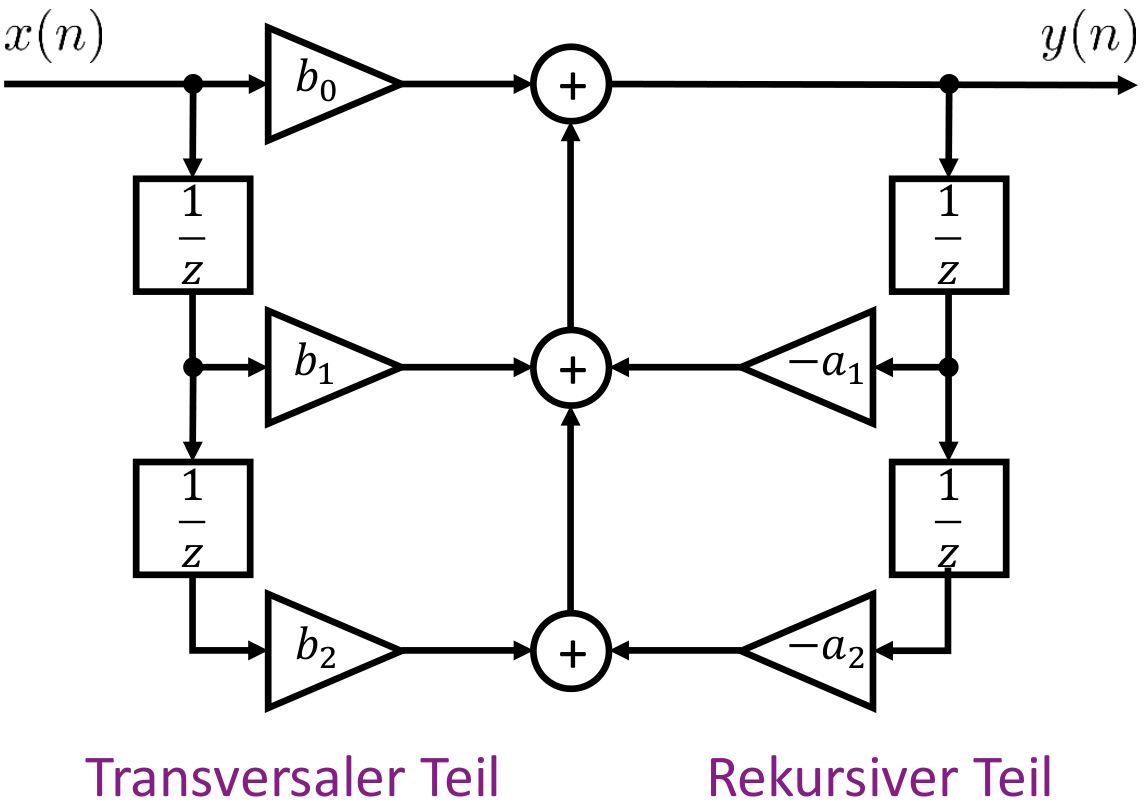
\includegraphics[width=\columnwidth]{Bilder/Signalfluss_plan-graph}
\end{minipage}
\begin{minipage}{0.5\columnwidth}
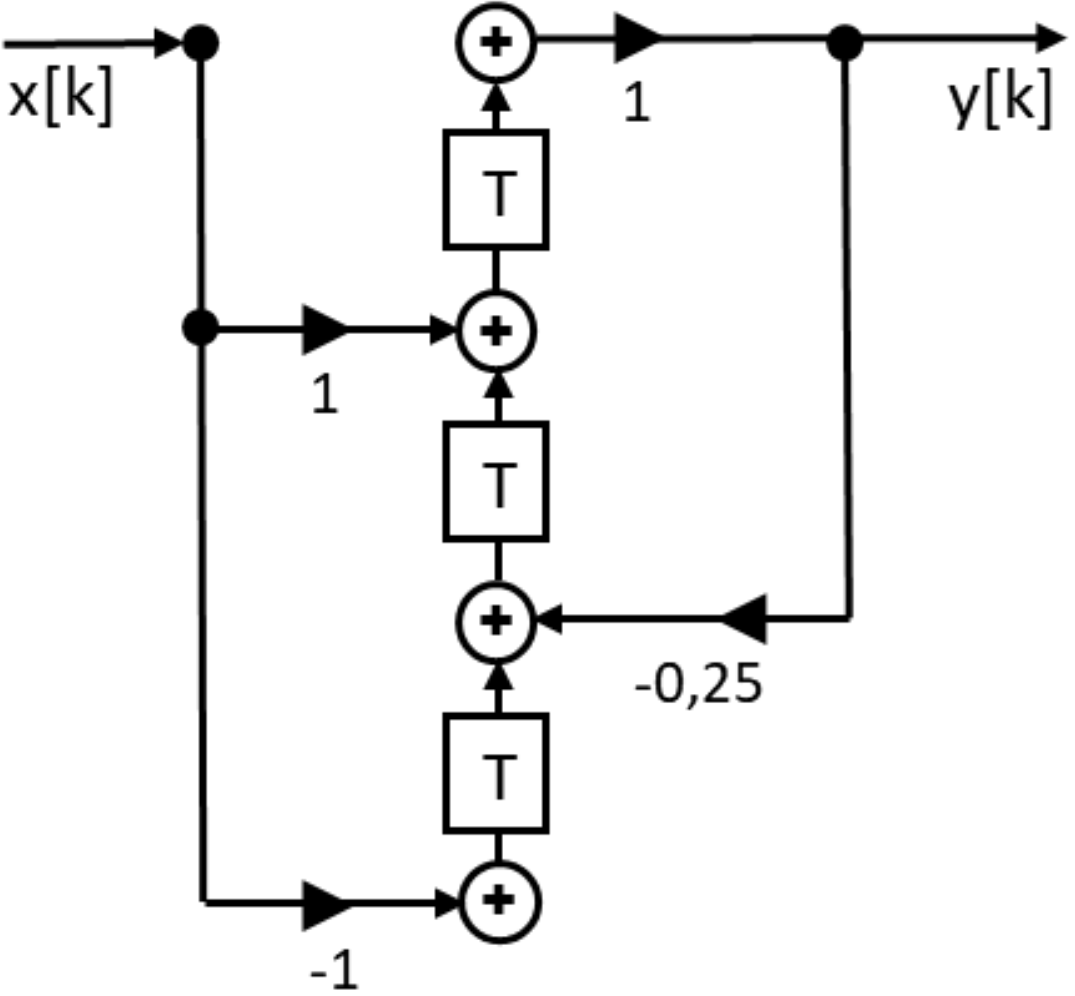
\includegraphics[width=\columnwidth]{Bilder/Signalflussdiagramm}
\end{minipage}

\subsection{Zeitdiskrete Signale im Spektrum}
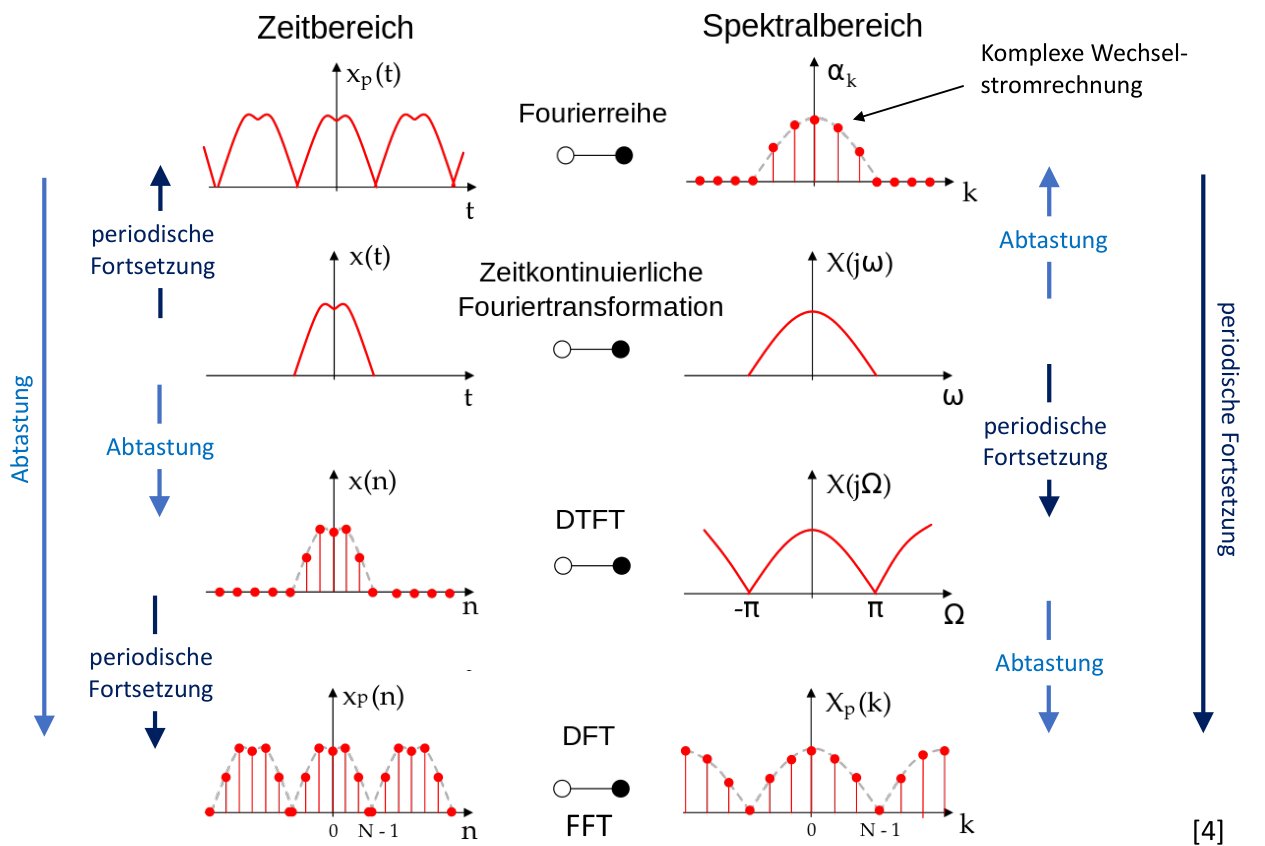
\includegraphics[width=\columnwidth]{Bilder/uebersicht_abtastung_frequenzbereich}
\clearpage
\subsection{Zeitdiskrete Fouriertransformation}
\begin{itemize}
\item zeitdiskrete Fouriertransformation (DTFT):
\[ \boxed{
\underline{X}(\Omega) = \sum_{n=-\infty}^{\infty} x(n) \cdot e^{-j\Omega n}
}
\]
\item Rücktransformation, Synthese:
\[
x(n) = \frac{1}{2\pi}\int_{-\pi}^{\pi} X(\Omega) \cdot  e^{j\Omega n} \, d\Omega
\]
\item Normierte Kreisfrequenz:
\[ \boxed{
\Omega = \omega T = 2\pi f T = 2\pi \frac{f}{f_a} }
\]
{\small Spektrum $\underline{X}(\Omega)$ ist freq.-kontinuierlich und\\ periodisch mit $T=2\pi$. $\rightarrow$ $X(\Omega)=X(\Omega+2\pi)$}
\item Einheit des Spektrums/Signals: $[\underline{X}(\omega)] = x(n)$
\end{itemize}

\subsection{z-Transformation}
Hintransformation, Analysegleichung: 
\[\boxed{
	\underline{X}(z) = \sum_{n=0}^{\infty} x(n) \cdot z^{-n} }
\]
Existiert nur für rechtsseitige (kausale) Folgen/Signale!
\small
\begin{itemize}
	\item Kb darf keine Polstellen enthalten.
	\item Zeitbegrenzte (kausale) Signale: Kb außerhalb\\ des Ursprungs.
	\item Unendlich lange (kausale) Signale: Kb außerhalb\\ des Kreises durch betragsgrößte Polstelle.
\end{itemize}
\normalsize

\subsubsection{Rücktransformation mit PBZ}
Partialbruchzerlegung allgemein:
\[
\underline{X}(z)=\frac{\underline{Z}(z)}{\underline{N}(z)}=\frac{\sum_{m=0}^{M} b_{m} z^{m}}{\sum_{n=0}^{N} a_{n} z^{n}}=\frac{b_{M}}{a_{N}} \cdot \frac{\prod_{m=1}^{M}\left(z-z_{o m}\right)}{\prod_{n=1}^{N}\left(z-z_{x n}\right)}
\]
\textbf{Einfache} Polstellen $p_n$:
\begin{align*}
	\Aboxed{\frac{\underline{X}(z)}{z} & =\frac{c_{0}}{z}+\frac{c_{1}}{z-z_{x 1}}+\frac{c_{2}}{z-z_{x 2}}+\cdots+\frac{c_{N}}{z-z_{x N}}} \\
	\Rightarrow \underline{X}(z) &= c_0 + \sum_{n=1}^{N} c_n \frac{z}{z-p_n} \quad c_0=0, \text{wenn } b_0=0
\end{align*}
Sonderfall: $n$-fache Polstellen bei $z=0$:
\begin{align*}
	\underline{X}(z) = \frac{\sum_{m=0}^{M} b_m \cdot  z^m}{a_N \cdot z^N} = \sum_{m=0}^{M} \frac{b_m}{a_N} \cdot z^{m-N}
\end{align*}
\textbf{Mehrfache} Polstellen $p_n$:
\begin{align*}
	\Aboxed{\frac{\underline{X}(z)}{z} &=\frac{c_{0}}{z}+\frac{c_{1}}{z-p_n}+\frac{c_{2}}{\left(z-p_n\right)^{2}}+\cdots+\frac{c_{k}}{\left(z-z_{x n}\right)^{k}}}\\
			\Rightarrow \underline{X}(z) & = c_0 + c_1 \frac{z}{z-p_n}+c_2\frac{z}{(z-p_n)^2}+\cdots+c_k\frac{z}{(z-p_n)^k}
\end{align*}

\subsubsection{Eigenschaften der z-Transformation}
\renewcommand{\arraystretch}{1.7}
{\small 
\begin{tabularx}{\columnwidth}{|c|c|c|}
	\hline
	& $\mathbf{x[n]}$ & \underline{$\mathbf{X}$}$\mathbf{(z)}$\\
	\hline Linearität & $a x_{1}[n]+b x_{2}[n]$ & $a \underline{X}_{1}(z)+b\underline{X}_{2}(z)$ \\
	\hline Verschiebung	& $x[n-k]$ & $z^{-k} \underline{X}(z)$ \\
	\hline Modulation & $a^{n} \, x[n]$ & $\underline{X}\left(\frac{z}{a}\right)$ \\
	\hline Multiplikation & $n \cdot x[n] $ & $-z \frac{d}{d z} \underline{X}(z)$ \\
	\hline Faltung & $x_{1}[n] * x_{2}[n] $ & $ \underline{X}_{1}(z) \cdot \underline{X}_{2}(z)$ \\
	\hline Faltung im BB & $x_{1}[n] \cdot x_{2}[n] $ & $ \frac{1}{2\pi j} \int \underline{X}_1(\eta)\underline{X}_2(\frac{z}{\eta})\frac{1}{\eta}\, d\eta$ \\
	\hline Differenzbildung & $x[n]-x[n-1] $ & $ \frac{z-1}{z} \underline{X}(z)$ \\
	\hline Summenbildung & $\sum_{i=0}^{n} x[i] $ & $ \frac{z}{z-1} \underline{X}(z)$ \\
	\hline
\end{tabularx} }

\subsubsection{Korrespondenzen der z-Transformation}
Normierte Kreisfrequenz $\Omega_1 = \omega T$\\
\renewcommand{\arraystretch}{1.7}
\begin{tabularx}{\columnwidth}{|l|X|X|}
	\hline $\mathbf{N r}$. & $\mathbf{x}[\mathbf{n}]$ & $\mathbf{\underline{X}}(\mathbf{z})$ \\
	\hline 1 & $\delta[n]$ & 1 \\
	\hline 2 & $\delta[n-i]$ & $z^{-i}$ \\
	\hline 3 & $\varepsilon[n]$ & $\frac{z}{z-1}$ \\
	\hline 4 & $\varepsilon[n-i]$ & $\frac{z}{z-1} \cdot z^{-i}$ \\
	\hline \textbf{5} & $n \cdot \varepsilon[n]$ & $\frac{z}{(z-1)^{2}}$ \\
	\hline 6 &  $n^2 \cdot \varepsilon[n]$ & $\frac{z(z+1)}{(z-1)^3}$  \\
\hline 7 & $e^{-a n} \cdot \varepsilon[n]$ & $\frac{z}{z-e^{-a}}$ \\
\hline 8 & $n \, e^{-a n} \cdot \varepsilon[n]$ & $\frac{z e^{-a}}{\left(z-e^{-a}\right)^{2}}$ \\
\hline \textbf{9} & $a^{n} \cdot \varepsilon[n]$ & $\frac{z}{z-a}$ \\
\hline 10 & $a^{n-1} \cdot \varepsilon[n-1]$ & $\frac{1}{z-a}$ \\
\hline \textbf{11} & $n\,a^{n} \cdot \varepsilon[n]$ & $\frac{z a}{(z-a)^{2}}$ \\
\hline 12 & $n \, a^{n-1} \cdot \varepsilon[n]$ & $\frac{z}{(z-a)^{2}}$ \\
\hline 13 & $(n-1) \, a^{n-1} \cdot \varepsilon[n-1]$ & $\frac{1}{(z-a)^{2}}$ \\
\hline 14 & $n^{2} \, a^{n} \varepsilon[n]$ & $\frac{a z(z+a)}{(z-a)^{3}}$ \\
\hline 15 & $\binom{n}{i} a^{n-i} \varepsilon[n-i]$ & $\frac{z}{(z-a)^{i+1}}$ \\
\hline 16 & $\frac{\left(a^{n+1}-b^{n+1}\right)}{a-b} \varepsilon[n] \quad a \neq b$ & $\frac{z^{2}}{(z-a)(z-b)}$ \\
\hline 17 & $\frac{1}{n} \varepsilon[n-1] \cdot \varepsilon[n]$ & $\ln \left(\frac{z}{z-1}\right)$ \\
\hline \textbf{18} & $\sin (\Omega_1 n ) \cdot \varepsilon[n]$ & $\frac{z \sin (\Omega_1)}{z^{2}-2 z \cos (\Omega_1)+1}$ \\
\hline \textbf{19} & $\cos (\Omega_1 n ) \cdot \varepsilon[n]$ & $\frac{z[z-\cos (\Omega_1)]}{z^{2}-2 z \cos (\Omega_1)+1}$ \\
\hline 20 & $a^{n} \sin (\Omega_1 n) \cdot \varepsilon[n]$ & $\frac{z a \sin (\Omega_1)}{z^{2}-2 z a \cos (\Omega_1)+a^{2}}$ \\
\hline 21 & $a^{n} \cos (\Omega_1 n) \cdot \varepsilon[n]$ & $\frac{z[z-a \cos (\Omega_1)]}{z^{2}-2 z a \cos (\Omega_1)+a^{2}}$ \\
\hline 22 & $\operatorname{rect}_{N}[n]$ & $\frac{z-z^{-N}}{z-1}$ \\
\hline
\end{tabularx}
\clearpage

\subsection{LTI-Systeme im Bildbereich}
\subsubsection{Impuls- und Sprungantwort im BB}
$$
	h(n) \, \laplace \, \boxed{\underline{H}(z) = \underline{G}(z) \cdot \frac{z-1}{z} } \qquad \boxed{
	\underline{G}(z) = \underline{H}(z) \cdot \frac{z}{z-1} }
$$




\subsubsection{PN-Diagramm $\Rightarrow$ Frequenzgang}
Wenn zeitdiskretes LTI-System \textbf{stabil}: Ersetze $z=e^{j\Omega}$:\\
\[ \boxed{
	\underline{H}(\Omega)=\left.\underline{H}(z)\right|_{z=e^{j \Omega}} } \quad \text{wenn \textbf{alle} Pole innerhalb des EK.}
\]
\textbf{Ermittlung} $\underline{H}(\Omega)$: Am Einheitskreis des PN-Diagramms \textit{entlang} gegen den UZS für $\Omega > 0$ gehen.\\

$z_o$: Nullstellen, \quad $z_x$: Polstellen
\begin{gather*}
	\underline{H}(z)=\frac{\left(z-z_{o}\right)}{\left(z-z_{x}\right)} \qquad
	\underline{H}(\Omega)=\frac{\left(e^{j \Omega}-z_{o}\right)}{\left(e^{j \Omega}-z_{x}\right)}=\frac{A_{o} e^{j \varphi_{o}}}{A_{x} e^{j \varphi_{x}}}
\end{gather*}
\centering
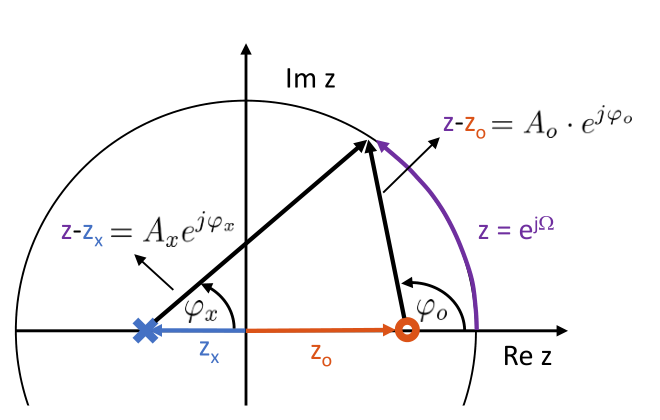
\includegraphics[width=0.7\columnwidth]{Bilder/PN-FreqGang}

\raggedright
\textbf{Betragsfrequenzgang}, Amplitudengang\\
Pole/Nullstellen $\rightarrow$ Amplitude steigt/sinkt.
\[
|\underline{H}(\Omega)| = H(\Omega)=\frac{A_{o}(\Omega)}{A_{x}(\Omega)} = \frac{Y(\Omega)}{X(\Omega)}
\]
\textbf{Phasenfrequenzgang}
\[
\varphi_{H}(\Omega)=\varphi_{o}(\Omega)-\varphi_{x}(\Omega) =\varphi_{Y}(\Omega)-\varphi_{X}(\Omega)
\]

Beispiele:
\makebox[\columnwidth][c]{
	\begin{minipage}{0.5\columnwidth}
		\begin{center}
			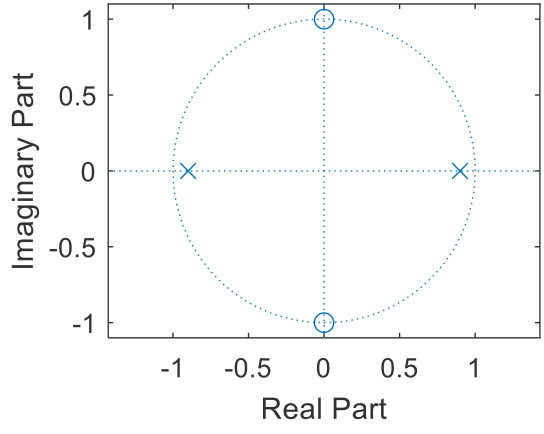
\includegraphics[width=0.9\columnwidth]{Bilder/PN-FreqGang_BSP-P1}
		\end{center}
	\end{minipage}
	\begin{minipage}{0.5\columnwidth}
		\begin{center}
			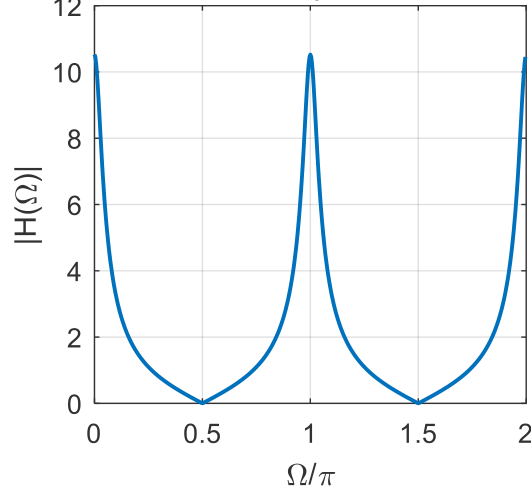
\includegraphics[width=0.8\columnwidth]{Bilder/PN-FreqGang_BSP-P2}
		\end{center}
	\end{minipage}
}
\makebox[\columnwidth][c]{
	\begin{minipage}{0.5\columnwidth}
		\begin{center}
			\includegraphics[width=0.9\columnwidth]{Bilder/PN-FreqGang_BSP1-P1}
		\end{center}
	\end{minipage}
	\begin{minipage}{0.5\columnwidth}
		\begin{center}
			\includegraphics[width=0.8\columnwidth]{Bilder/PN-FreqGang_BSP2-P2}
		\end{center}
	\end{minipage}
}

\subsubsection{Systemantwort auf harm. Eingangssignale}	
LTI-System verändert \textbf{nur} Amplitude und Phase von $x(t)$.\\
Normierte Frequenz $\Omega_1 = \omega T$ bleibt gleich.

\begin{tabular}{cc}
	Gegeben: & $x(n) = \hat{x} \cdot \sin(\Omega_1n+\varphi_x)+x_0$\\
	Gesucht: & $y(n) = \hat{y} \cdot \sin(\Omega_1n+\varphi_y)+x_0$
\end{tabular}
\begin{gather*}
\boxed{
\hat{y} = \hat{x} \cdot |\underline{H}(\Omega_1)|} \qquad
\boxed{
 \varphi_y = \varphi_x + \varphi_H(\Omega_1) } 
\end{gather*}



%\end{multicols*}
%\subsection{s-Frequenzebene/z-Frequenzebene}
%\begin{center}
%	\begin{tabular}[htpb]{c|c|c}
%		s-Frequenzebene     & $e^{sT} = z$          & z-Frequenzebene     \\
%		\hline
%		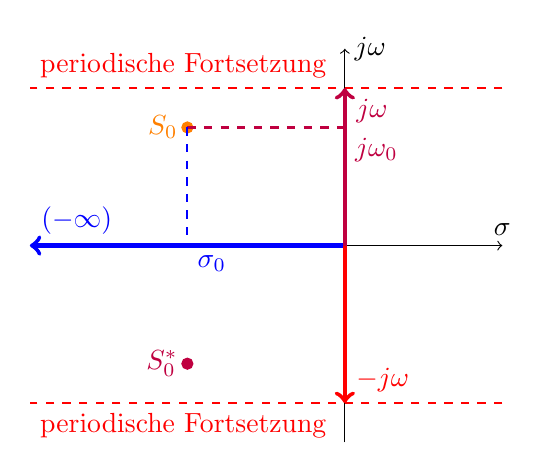
\begin{tikzpicture}[baseline=1]
    \draw[->] (0,-2.5) -- (0,2.5) node[right]{$j\omega$}; %y
    \draw[->] (-4,0) -- (2,0) node[above]{$\sigma$}; %x

    \draw[thick, dashed, red] (2,2) -- (-4,2) node[above right]{periodische Fortsetzung};
    \draw[thick, dashed, red] (2,-2) -- (-4,-2) node[below right]{periodische Fortsetzung};
    \draw[ultra thick, ->, blue] (0,0) -- (-4,0) node[above right]{$(-\infty)$};
    \draw[ultra thick, ->, purple] (0,0) -- (0,2) node[below right]{$j \omega$};
    \draw[ultra thick, ->, red] (0,0) -- (0,-2) node[above right]{$-j \omega$};

    \filldraw[orange] (-2,1.5) circle (2pt) node[left]{$S_0$};
    \draw[thick, dashed, purple] (-2,1.5) -- (0,1.5) node[below right]{$j \omega_0 $};
    \draw[thick, dashed, blue] (-2,1.5) -- (-2,0) node[below right]{$ \sigma_0 $};

    \filldraw[purple] (-2,-1.5) circle (2pt) node[left]{$S_0^*$};
\end{tikzpicture}
 & $\Rightarrow$ & 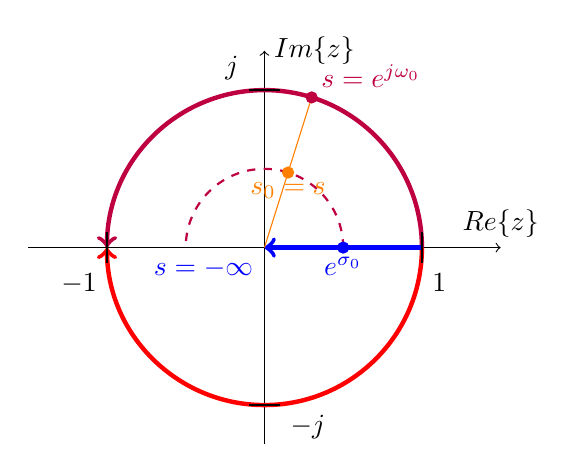
\begin{tikzpicture}[baseline=1]
    \draw[->] (0,-2.5) -- (0,2.5) node[right]{$\mathfrak{Im}\{z\}$}; %y
    \draw[->] (-3,0) -- (3,0) node[above]{$\mathfrak{Re}\{z\}$}; %x

    \draw[thick, color=black, dashed](0,0) circle (2);
    \draw[ultra thick, ->, purple] (2,0) arc (0:180:2);
    \draw[ultra thick, ->, red] (2,0) arc (0:-180:2);
    \draw[ultra thick, ->, blue] (2,0) -- (0,0) node[below left]{$s =-\infty$};

    \draw[thick, dashed, purple] (1,0) arc (0:180:1);

    \draw[thick, black] (0.2,2) -- (-0.2,2) node[above left]{$j$};
    \draw[thick, black] (-0.2,-2) -- (0.2,-2) node[below right]{$-j$};
    \draw[thick, black] (2,0.2) -- (2,-0.2) node[below right]{$1$};
    \draw[thick, black] (-2,0.2) -- (-2,-0.2) node[below left]{$-1$};

    \filldraw[blue] (1,0) circle (2pt) node[below]{$ e^{\sigma_0}$};
    \filldraw[orange] (0.3,0.953) circle (2pt) node[below]{$s_0 = s$};
    \draw[orange] (0,0) -- (0.6,1.907) {};
    \filldraw[purple] (0.6,1.907) circle (2pt) node[above right]{$s=e^{j \omega_0}$};
\end{tikzpicture}
 \\
%	\end{tabular}
%\end{center}
%\begin{multicols*}{2}
%\subsection{s-Frequenzebene/z-Frequenzebene}

\subsubsection{Klassifizierung von Systemen}
% Die mathematischen Beschreibung fehlen. wurden nie gebraucht während lernen. Kap6S63 6.5.7
\begin{itemize}[leftmargin=*]
	\item \textbf{Transversale Systeme}, FIR, AR:
	
	{\small Finite Impulse Response (FIR), Auto-Regressive (AR)\\
		Keine Rückführung von Ausgang $y(n)$ auf Eingang $x(n)$.}\\
	$\Rightarrow$ $a_k=0 \texttt{ für } k>0$.\\
	$\Rightarrow$ Alle Pole liegen im Ursprung.
	
	\makebox[\columnwidth][c]{
		\begin{minipage}{0.5\columnwidth}
			\includegraphics[width=0.7\columnwidth]{Bilder/Transversale_Systeme_}
		\end{minipage}
		\hspace{-1em}
		\begin{minipage}{0.5\columnwidth}
			\includegraphics[width=0.8\columnwidth]{Bilder/Transversale_Systeme_SG}
		\end{minipage}
	}
	
	\item \textbf{Rekursive Systeme}, IIR, MA:
	
	{\small Infinite Impulse Response (IIR), Moving-Average (AR)\\
		Aktueller Ausgangswert hängt nur vom aktuellen Eingangswert
		und früheren Ausgangswerten ab.}\\
	$\Rightarrow$ $b_k=0 \texttt{ für } k>0$.\\
	$\Rightarrow$ Alle Nullstellen liegen im Ursprung.
	
	\makebox[\columnwidth][c]{
		\begin{minipage}{0.5\columnwidth}
			\includegraphics[width=0.7\columnwidth]{Bilder/Rekursive_Systeme}
		\end{minipage}
		\hspace{-1em}
		\begin{minipage}{0.5\columnwidth}
			\includegraphics[width=0.8\columnwidth]{Bilder/Rekursive_Systeme_SG}
		\end{minipage}
	}
	\item ARMA: Auto-Regressive Moving Average\\ $\rightarrow$ transversal-rekursives System.
\end{itemize}



% \newpage
% \section{Wichtige Formeln aus der Vorlesung}
% \textbf{Integral über die Gaußische kurve}:
%     \[
%         \int_{-\infty}^{\infty} e^{\frac{-1}{2\sigma^2}t^2}dt \overset{2.3}{=}
%         \sqrt{2\cdot\pi\sigma^2}
%     \]

\end{multicols*}
\end{document}
